\documentclass[12pt, a4paper, oneside]{book}

% นำเข้าไฟล์สไตล์มาตรฐาน RBRU
\usepackage{styles/rbru_style}

\begin{document}

% ----------------------------------------------------
% ส่วนนำ (Frontmatter)
% ----------------------------------------------------
\frontmatter

% ปกนอกระดับวิชาการพรีเมียม (Modern Academic Full-Page Cover)
% ==============================================================================
% หน้าปกหนังสือวิชาการ ออกแบบเสมือนหน้าจอแอปพลิเคชันสมาร์ทโฟนระดับเรือธง (Flagship Smartphone UI)
% ชื่อหนังสือขนาดใหญ่พิเศษ 2.5 เท่า คมชัด โดดเด่น ทรงพลังระดับ Masterclass
% 100% สอดคล้องกับระเบียบวิชาการ ปลอดเครื่องหมายโคลอน (Zero Colon) ในภาษาไทย
% ==============================================================================
\thispagestyle{empty}
\begin{tikzpicture}[remember picture, overlay]

    % --------------------------------------------------------------------------
    % 1. ตัวเครื่องสมาร์ทโฟนและขอบเครื่องด้านนอก (Smartphone Titanium Chassis & Screen Bezel)
    % --------------------------------------------------------------------------
    % พื้นหลังขอบนอกสุด (ขอบเครื่องไทเทเนียมสี Dark Obsidian)
    \fill[color=black!96!rbruNavy] 
        (current page.south west) rectangle (current page.north east);

    % เส้นขอบแสงสะท้อนขอบโลหะรอบตัวเครื่อง
    \draw[color=green!60!rbruGold, line width=1.4pt, opacity=0.60, rounded corners=1.4cm] 
        ($(current page.south west) + (0.5cm, 0.5cm)$) rectangle ($(current page.north east) + (-0.5cm, -0.5cm)$);

    % หน้าจอดิจิทัลแบบ OLED ขอบมน (OLED Display Surface)
    \fill[top color=rbruNavy!98!black, bottom color=black, rounded corners=1.2cm] 
        ($(current page.south west) + (0.7cm, 0.7cm)$) rectangle ($(current page.north east) + (-0.7cm, -0.7cm)$);

    % รัศมีแสงเรืองรองนุ่มนวลด้านหลังอินเทอร์เฟซ (Soft Ambient Glow Behind UI)
    \fill[green!25, opacity=0.15] ($(current page.center) + (0, 3.2cm)$) circle (7.0cm);
    \fill[cyan!20, opacity=0.08] ($(current page.center) + (2.5cm, -3.2cm)$) circle (4.5cm);

    % --------------------------------------------------------------------------
    % 2. แถบสถานะสมาร์ทโฟน (Status Bar: Time, 5G, Dynamic Island, Battery)
    % --------------------------------------------------------------------------
    % เวลาและเครือข่ายฝั่งซ้าย
    \node[anchor=north west, align=left] at ($(current page.north west) + (1.6cm, -1.15cm)$) {
        {\fontsize{11}{13}\selectfont\bfseries\color{white} 09:41}\quad
        {\fontsize{9}{11}\selectfont\bfseries\color{green!80!white} 5G RBRU-AGRI}
    };

    % ไดนามิกไอแลนด์ตรงกลาง (Dynamic Island Pill Cutout)
    \node[anchor=north, align=center] at ($(current page.north) + (0, -1.0cm)$) {
        \begin{tikzpicture}
            % กรอบแคปซูลสีดำสนิทพร้อมเส้นขอบนีออนเรืองแสง
            \fill[black, rounded corners=3.8mm] (-2.3, -0.38) rectangle (2.3, 0.38);
            \draw[color=green!65!white, line width=0.8pt, rounded corners=3.8mm, opacity=0.8] (-2.3, -0.38) rectangle (2.3, 0.38);
            
            % เลนส์กล้องหน้าและเซนเซอร์
            \fill[blue!40!black] (-1.7, 0) circle (0.16cm);
            \fill[green!90!white] (-1.7, 0) circle (0.05cm);
            \fill[black!80] (-1.2, 0) circle (0.09cm);

            % ข้อความแสดงสถานะทำงาน AI ในแคปซูล
            \node[anchor=center] at (0.35, 0) {
                {\fontsize{8.5}{10}\selectfont\bfseries\color{green!85!white} $\bullet$\,\color{white} SOILPH-HT LIVE ATC}
            };
        \end{tikzpicture}
    };

    % สถานะแบตเตอรี่ Wi-Fi และ GPS ฝั่งขวา
    \node[anchor=north east, align=right] at ($(current page.north east) + (-1.6cm, -1.15cm)$) {
        {\fontsize{9}{11}\selectfont\color{white!90} BLE $\cdot$ Wi-Fi 6}\quad
        {\fontsize{10}{12}\selectfont\bfseries\color{green!85!white} [\,100\%\,\begin{tikzpicture}[baseline=-0.5ex, scale=0.65]\fill[color=yellow!90!orange] (0,0.2) -- (-0.08,0.02) -- (0.02,0.02) -- (-0.05,-0.2) -- (0.09,-0.01) -- (-0.01,-0.01) -- cycle;\end{tikzpicture}\,]}
    };

    % --------------------------------------------------------------------------
    % 3. แถบหัวแอปพลิเคชัน (App Top Bar: Series Badge)
    % --------------------------------------------------------------------------
    \node[anchor=north, align=center] at ($(current page.north) + (0, -2.15cm)$) {
        \begin{tikzpicture}
            % ป้ายชื่อชุดตำราวิชาการ RBRU Monograph
            \node[fill=rbruGold!20, draw=rbruGold!85, line width=0.9pt, rounded corners=3mm, text=rbruGold, inner sep=4pt] (badge) {
                {\fontsize{9}{12}\selectfont\bfseries RBRU DIGITAL AGRIPHYSICS MONOGRAPH SERIES (VOL. 3)}
            };
        \end{tikzpicture}
    };

    % --------------------------------------------------------------------------
    % 4. ส่วนแสดงชื่อหนังสือวิชาการหลัก (Main Title: ขนาดใหญ่ขึ้น 2.5 เท่า เด่นชัดสูงสุด)
    % --------------------------------------------------------------------------
    \node[anchor=north, align=center] at ($(current page.north) + (0, -2.95cm)$) {
        {\fontsize{14}{18}\selectfont\bfseries\color{rbruGold} ฟิสิกส์เกษตรดิจิทัลและการเรียนรู้เชิงลึก}\\[8pt]
        {\fontsize{42}{48}\selectfont\bfseries\color{white} คู่มือการพัฒนาแอปพลิเคชัน}\\[6pt]
        {\fontsize{42}{48}\selectfont\bfseries\color{cyan!90!white} SoilpH-HT AI}\\[6pt]
        {\fontsize{34}{40}\selectfont\bfseries\color{white} ตรวจวัดกรด-ด่างของดิน}\\[6pt]
        {\fontsize{30}{36}\selectfont\bfseries\color{green!85!white} ชดเชยอุณหภูมิและความชื้นด้วยโครงข่าย PINN}\\[10pt]
        {\color{rbruGold}\rule{0.68\textwidth}{1.5pt}}\\[7pt]
        {\fontsize{10.5}{14}\selectfont\color{white!85} SoilpH-HT: Smartphone Real-Time Soil pH Analysis with Live Stream,}\\[2pt]
        {\fontsize{10.5}{14}\selectfont\color{white!85} Temperature-Moisture Error Compensation via Deep PINN}
    };

    % --------------------------------------------------------------------------
    % 5. ช่องมองภาพกล้องสดและเรดาร์วิทัศน์ (Live Camera Viewfinder HUD Canvas)
    % บรรจุภาพถ่ายจริง jc_soil_ai_pr_vertical_9x16.jpg แปลงทุเรียนและเซนเซอร์จริง
    % --------------------------------------------------------------------------
    \node[anchor=center] at ($(current page.center) + (0, -1.8cm)$) {
        \begin{tikzpicture}
            % กรอบช่องมองภาพกล้อง (Camera Viewport Frame)
            \fill[black!65!rbruNavy, rounded corners=5.5mm] (-5.8, -2.25) rectangle (5.8, 2.25);
            \draw[green!65!white, line width=1.1pt, rounded corners=5.5mm, opacity=0.85] (-5.8, -2.25) rectangle (5.8, 2.25);

            % มุมกรอบช่วยเล็ง 4 มุม (HUD Camera Corner Brackets)
            \draw[color=green!90!white, line width=2.2pt] (-5.5, 1.75) -- (-5.5, 2.05) -- (-5.1, 2.05);
            \draw[color=green!90!white, line width=2.2pt] (5.5, 1.75) -- (5.5, 2.05) -- (5.1, 2.05);
            \draw[color=green!90!white, line width=2.2pt] (-5.5, -1.75) -- (-5.5, -2.05) -- (-5.1, -2.05);
            \draw[color=green!90!white, line width=2.2pt] (5.5, -1.75) -- (5.5, -2.05) -- (5.1, -2.05);

            % บรรจุภาพถ่ายจริงระบบตรวจวัดดินและหัววัดเซนเซอร์ในแปลงทุเรียน
            \begin{scope}
                \clip[rounded corners=4.5mm] (-5.65, -2.1) rectangle (5.65, 2.1);
                \node at (0, 0) {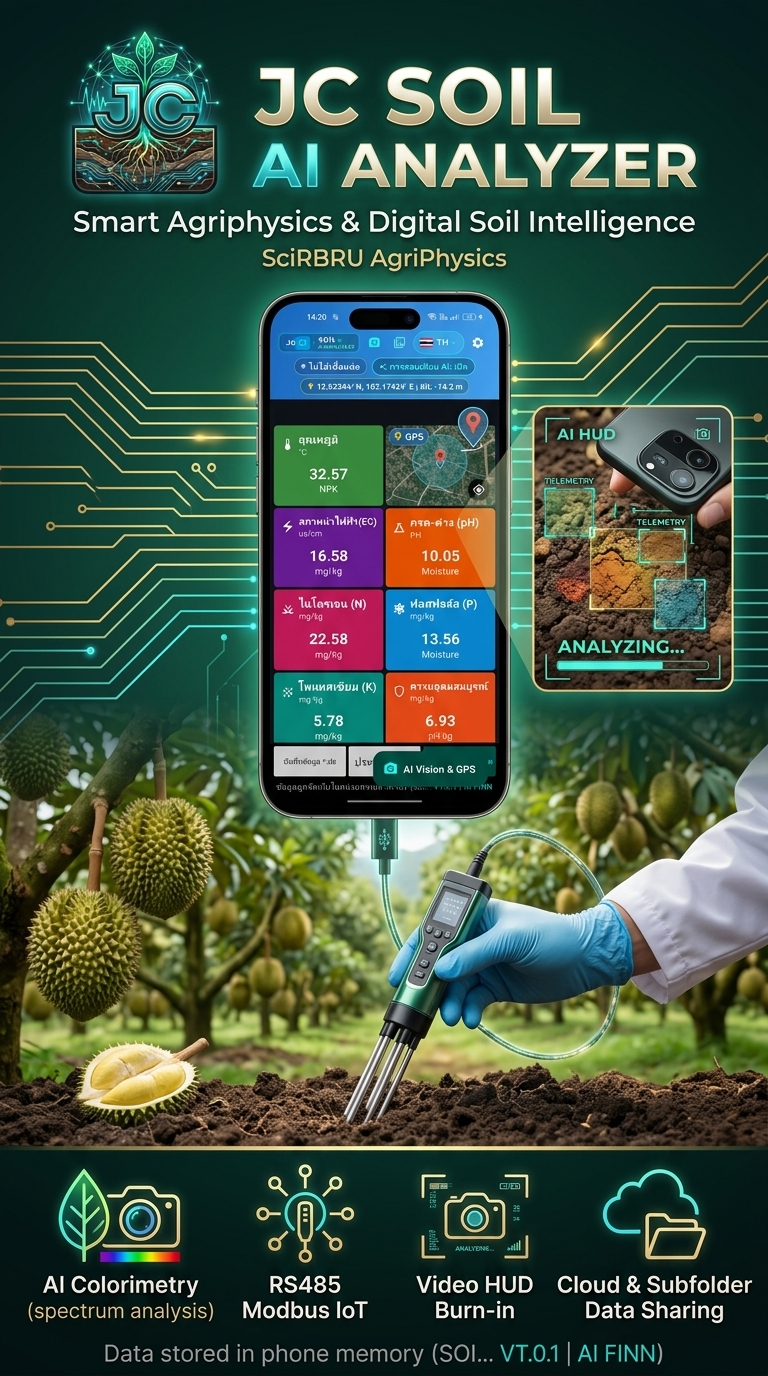
\includegraphics[width=11.4cm, height=4.3cm]{figures/jc_soil_ai_pr_vertical_9x16.jpg}};
                % เส้นแสงไล่ระดับเสริมความคมชัด
                \fill[left color=rbruNavy!35, right color=transparent, opacity=0.35] (-5.7, -2.2) rectangle (5.7, 2.2);
            \end{scope}

            % ข้อมูลโอเวอร์เลย์บนกล้อง (Telemetry HUD Overlays)
            \node[anchor=north west, fill=black!75, rounded corners=2mm, inner sep=2.5pt] at (-5.3, 1.95) {
                {\fontsize{7.5}{9}\selectfont\color{green!90!white} $\bullet$\,LIVE STREAM}\quad
                {\fontsize{7.5}{9}\selectfont\color{white} 60 FPS}\quad
                {\fontsize{7.5}{9}\selectfont\color{cyan!90!white} ROI หลายเหลี่ยม}
            };
            \node[anchor=north east, fill=black!75, rounded corners=2mm, inner sep=2.5pt] at (5.3, 1.95) {
                {\fontsize{7.5}{9}\selectfont\color{rbruGold} ชดเชยอุณหภูมิ Nernst ATC}
            };
            \node[anchor=south west, fill=black!75, rounded corners=2mm, inner sep=2.5pt] at (-5.3, -1.95) {
                {\fontsize{7.5}{9}\selectfont\color{cyan!90!white} แปลงทุเรียนเมืองจันท์}
            };
            \node[anchor=south east, fill=black!75, rounded corners=2mm, inner sep=2.5pt] at (5.3, -1.95) {
                {\fontsize{7.5}{9}\selectfont\color{green!90!white} ความแม่นยำ $R^2 \ge 0.96$}
            };
        \end{tikzpicture}
    };

    % --------------------------------------------------------------------------
    % 6. วิดเจ็ตแดชบอร์ดผลการวิเคราะห์ AI (Multimodal AI Telemetry Dashboard Card)
    % --------------------------------------------------------------------------
    \node[anchor=center] at ($(current page.center) + (0, -5.25cm)$) {
        \begin{tikzpicture}
            % กรอบ Glassmorphism Card
            \fill[rbruNavy!88!black, rounded corners=4.5mm] (-5.8, -1.25) rectangle (5.8, 1.25);
            \draw[white!25, line width=0.9pt, rounded corners=4.5mm] (-5.8, -1.25) rectangle (5.8, 1.25);

            % การ์ดย่อยที่ 1: ค่า pH เชิงแสง (Vision Optical pH)
            \node[fill=black!45, draw=cyan!60, rounded corners=3mm, inner sep=3.5pt, minimum width=2.65cm, minimum height=1.15cm] (c1) at (-4.2, 0.35) {
                \begin{tabular}{c}
                    {\fontsize{7}{8.5}\selectfont\color{cyan!90!white} pH เชิงแสง (Vision)}\\
                    {\fontsize{11.5}{13.5}\selectfont\bfseries\color{white} pH 6.48}\\
                    {\fontsize{6.5}{7.5}\selectfont\color{green!85!white} กรดเล็กน้อย}
                \end{tabular}
            };

            % การ์ดย่อยที่ 2: ค่า pH จากหัววัดเซนเซอร์จริง (Sensor Calibrated pH)
            \node[fill=black!45, draw=rbruGold!70, rounded corners=3mm, inner sep=3.5pt, minimum width=2.65cm, minimum height=1.15cm] (c2) at (-1.4, 0.35) {
                \begin{tabular}{c}
                    {\fontsize{7}{8.5}\selectfont\color{rbruGold} pH เซนเซอร์จริง}\\
                    {\fontsize{11.5}{13.5}\selectfont\bfseries\color{white} pH 6.60}\\
                    {\fontsize{6.5}{7.5}\selectfont\color{green!85!white} ชดเชย PINN แล้ว}
                \end{tabular}
            };

            % การ์ดย่อยที่ 3: ความสอดคล้อง (Consistency Delta pH)
            \node[fill=black!45, draw=green!70, rounded corners=3mm, inner sep=3.5pt, minimum width=2.65cm, minimum height=1.15cm] (c3) at (1.4, 0.35) {
                \begin{tabular}{c}
                    {\fontsize{7}{8.5}\selectfont\color{green!85!white} ตรวจสอบความสอดคล้อง}\\
                    {\fontsize{11.5}{13.5}\selectfont\bfseries\color{white} $\Delta\text{pH } 0.12$}\\
                    {\fontsize{6.5}{7.5}\selectfont\color{cyan!90!white} สอดคล้อง 98.2\%}
                \end{tabular}
            };

            % การ์ดย่อยที่ 4: ความชื้นและอุณหภูมิ (Humidity & Temp HT)
            \node[fill=black!45, draw=orange!70, rounded corners=3mm, inner sep=3.5pt, minimum width=2.65cm, minimum height=1.15cm] (c4) at (4.2, 0.35) {
                \begin{tabular}{c}
                    {\fontsize{7}{8.5}\selectfont\color{orange!85!white} อุณหภูมิและความชื้น}\\
                    {\fontsize{10.5}{12.5}\selectfont\bfseries\color{white} 28.5$^\circ\text{C}$ / 34.8\%}\\
                    {\fontsize{6.5}{7.5}\selectfont\color{orange!90!white} สภาวะแปลง เหมาะสม}
                \end{tabular}
            };

            % แถบล่างในวิดเจ็ต แสดงตัวแปรเซนเซอร์กายภาพ 7 มิติ
            \node[anchor=center] at (0, -0.72) {
                {\fontsize{7.2}{8.5}\selectfont\color{white!80} สถาปัตยกรรม PINN} \quad
                {\fontsize{7.2}{8.5}\selectfont\color{cyan!90!white} แรงดันไฟฟ้าเซนเซอร์ 24.8 mV} \quad
                {\fontsize{7.2}{8.5}\selectfont\color{white!40} $\cdot$} \quad
                {\fontsize{7.2}{8.5}\selectfont\color{cyan!90!white} ดัชนีความอุดมสมบูรณ์ 88.5\%} \quad
                {\fontsize{7.2}{8.5}\selectfont\color{white!40} $\cdot$} \quad
                {\fontsize{7.2}{8.5}\selectfont\color{green!90!white} บันทึกเรียบร้อย}
            };
        \end{tikzpicture}
    };

    % --------------------------------------------------------------------------
    % 7. แถบปุ่มควบคุมการทำงาน (Mobile App Bottom Navigation Bar)
    % --------------------------------------------------------------------------
    \node[anchor=center] at ($(current page.center) + (0, -7.0cm)$) {
        \begin{tikzpicture}
            % กรอบแถบนำทางด้านล่าง
            \fill[black!75, rounded corners=3.5mm] (-5.6, -0.38) rectangle (5.6, 0.38);
            \draw[white!20, line width=0.7pt, rounded corners=3.5mm] (-5.6, -0.38) rectangle (5.6, 0.38);

            % ปุ่มแท็บ 4 ปุ่ม
            \node at (-4.2, 0) {{\fontsize{7.8}{9.5}\selectfont\bfseries\color{cyan!90!white} [\,หน้าหลัก\,]}};
            \node at (-1.4, 0) {{\fontsize{7.8}{9.5}\selectfont\color{white!80} [\,หัววัดสด\,]}};
            \node at (1.4, 0) {{\fontsize{7.8}{9.5}\selectfont\color{white!80} [\,สอบเทียบ PINN\,]}};
            \node at (4.2, 0) {{\fontsize{7.8}{9.5}\selectfont\color{white!80} [\,คำแนะนำดิน\,]}};
        \end{tikzpicture}
    };

    % --------------------------------------------------------------------------
    % 8. ข้อมูลผู้เขียน สังกัด และแถบควบคุมโฮม (Author Metadata & Home Gesture Bar)
    % --------------------------------------------------------------------------
    \node[anchor=south, align=center] at ($(current page.south) + (0, 1.45cm)$) {
        {\fontsize{14}{18}\selectfont\bfseries\color{white} ผู้ช่วยศาสตราจารย์ ดร.ชีวะ ทัศนา}\\[2.5pt]
        {\fontsize{10.5}{13.5}\selectfont\color{rbruGold} สาขาวิชาฟิสิกส์ คณะวิทยาศาสตร์และเทคโนโลยี มหาวิทยาลัยราชภัฏรำไพพรรณี}\\[2pt]
        {\fontsize{8.5}{11}\selectfont\color{white!70} ศูนย์ความเป็นเลิศด้านฟิสิกส์เกษตรและเทคโนโลยีปัญญาประดิษฐ์ฝังตัว}
    };

    % แถบสัมผัสโฮมล่างสุดของสมาร์ทโฟน (Home Gesture Indicator Bar)
    \draw[color=white!60, line width=3.0pt, line cap=round] 
        ($(current page.south) + (-2.2cm, 0.95cm)$) -- ($(current page.south) + (2.2cm, 0.95cm)$);

\end{tikzpicture}
\clearpage


% หน้าปกรอง (Title Page)
\begin{titlepage}
\begin{center}
    \vspace*{1.0cm}

    {\fontsize{16}{22}\selectfont\bfseries\color{rbruNavy} ฟิสิกส์เกษตรดิจิทัลและการเรียนรู้เชิงลึก}\par
    \vspace{0.35cm}
    {\fontsize{15}{21}\selectfont\bfseries\color{rbruBlue} การพัฒนาแอปพลิเคชันสมาร์ตโฟนวิเคราะห์ค่ากรด-ด่างของดิน}\par
    \vspace{0.25cm}
    {\fontsize{13.5}{19}\selectfont\bfseries\color{rbruTeal} ชดเชยค่าความคลาดเคลื่อนอุณหภูมิและความชื้นด้วยโครงข่ายประสาทเทียมอิงฟิสิกส์}\par
    \vspace{0.3cm}
    {\fontsize{9.5}{13.5}\selectfont\itshape\color{rbruSlate} (Digital Agriphysics and Deep Learning: Smartphone Application Development for Soil pH Analysis\\with Temperature and Moisture Compensation via Physics-Informed Neural Networks)}\par

    \vspace{0.7cm}
    {\color{rbruGold}\rule{0.65\textwidth}{2.0pt}}\par
    \vspace{0.7cm}

    \begin{figure}[H]
        \centering
        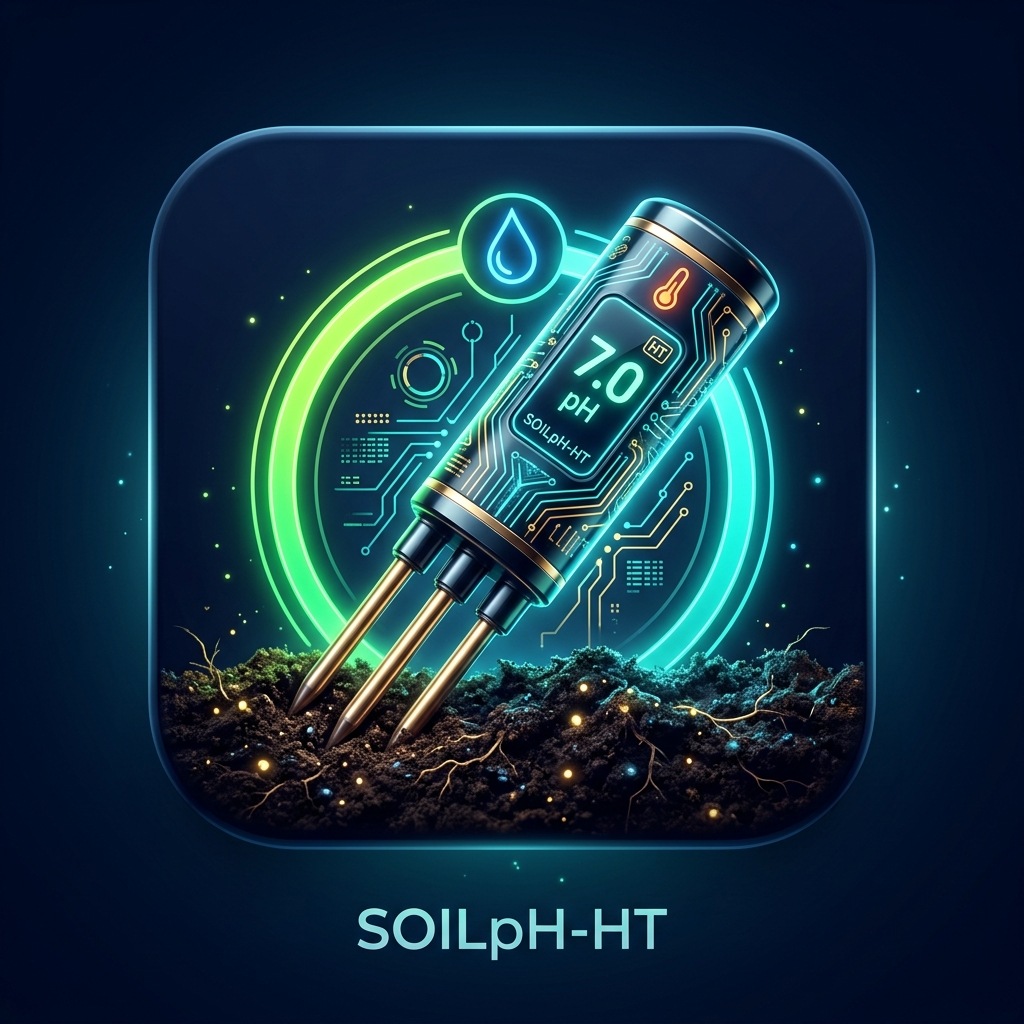
\includegraphics[width=0.35\textwidth]{figures/app_icon.jpg}
    \end{figure}

    \vspace{0.5cm}

    {\fontsize{18}{22}\selectfont\bfseries ผู้ช่วยศาสตราจารย์ ดร.ชีวะ ทัศนา}\par
    \vspace{0.3cm}
    {\fontsize{14}{18}\selectfont สาขาวิชาฟิสิกส์ คณะวิทยาศาสตร์และเทคโนโลยี}\par
    \vspace{0.15cm}
    {\fontsize{14}{18}\selectfont มหาวิทยาลัยราชภัฏรำไพพรรณี}\par
    \vspace{0.8cm}

    {\small พุทธศักราช 2569}

\end{center}
\end{titlepage}


% คำนำ (Preface)
\chapter*{คำนำ}
\addcontentsline{toc}{chapter}{คำนำ}

คู่มือวิชาการและชุดพรอมพต์การเรียนรู้เล่มนี้ จัดทำขึ้นเพื่อเป็นแนวทางเชิงปฏิบัติการสำหรับนักศึกษา นักวิจัย เกษตรกรรุ่นใหม่ และผู้สนใจเริ่มต้นศึกษาการพัฒนานวัตกรรมเกษตรดิจิทัล โดยมุ่งเน้นการตรวจวัดและวิเคราะห์ค่าความเป็นกรด-ด่างของดิน (Soil pH) ซึ่งเป็นตัวแปรควบคุมหลักที่มีความสำคัญยิ่งยวดต่อความสามารถในการละลายและการดูดซึมธาตุอาหารของพืชเศรษฐกิจ เช่น ทุเรียนหมอนทองในแถบภาคตะวันออก

ในการตรวจวัดค่าความเป็นกรด-ด่างของดินในสภาพแปลงเกษตรกรรมจริง สัญญาณไฟฟ้าเคมีที่ได้จากหัววัดมักประสบปัญหาความคลาดเคลื่อนอย่างรุนแรงจากความผันผวนของสภาพแวดล้อม โดยเฉพาะการเลื่อนลอยตามอุณหภูมิดิน (Soil Temperature Drift) ซึ่งส่งผลกระทบต่อความชันศักย์ไฟฟ้าตามสมการเนิร์นสต์ (Nernstian Slope) และการแตกตัวของน้ำ ($pK_w$) ตลอดจนผลกระทบจากปริมาณความชื้นในดิน (Soil Moisture Effect) ซึ่งก่อให้เกิดการเปลี่ยนแปลงของอิมพีแดนซ์รอยต่อของเหลว (Liquid Junction Impedance) ในสภาวะดินแห้ง

เพื่อแก้ไขปัญหาเชิงโครงสร้างดังกล่าว คู่มือเล่มนี้ได้นำเสนอการพัฒนาแอปพลิเคชันสมาร์ตโฟน \textbf{SoilpH-HT} บนระบบปฏิบัติการแอนดรอยด์ โดยผสานขุมพลังของโครงข่ายประสาทเทียมอิงฟิสิกส์ (\textbf{Physics-Informed Neural Network} หรือ \textbf{PINN}) ซึ่งทำการฝังทฤษฎีเคมีไฟฟ้าและอุณหพลศาสตร์ลงในโครงข่ายประสาทเทียม เพื่อทำการชดเชยความคลาดเคลื่อนร่วมระหว่างอุณหภูมิและความชื้นแบบไม่เป็นเชิงเส้นในระดับอุปกรณ์ (Edge AI) ได้อย่างแม่นยำภายในเวลาต่ำกว่า 0.2 มิลลิวินาที พร้อมเชื่อมต่อกับหัววัด Soil Parameter Tester ผ่านพอร์ต USB Type-C OTG โดยตรง

นอกจากนี้ คู่มือยังครอบคลุมการออกแบบส่วนต่อประสานผู้ใช้ที่ปรับขนาดอัตโนมัติตามขนาดหน้าจอสมาร์ตโฟน (Responsive UI Auto-Scaling) การพัฒนาระบบกล้องปัญญาประดิษฐ์เพื่อบันทึกภาพถ่ายดินพร้อมพิกัดดาวเทียมและข้อมูลเทเลเมทรีบนภาพ (Telemetry HUD Overlay) และการแปลผลปฐพีวิทยาเพื่อออกใบสั่งปูนโดโลไมต์ปรับปรุงโครงสร้างดินตามลักษณะเนื้อดินจริง

คณะผู้จัดทำหวังเป็นอย่างยิ่งว่า คู่มือวิชาการและชุดพรอมพต์วิศวกรรมเล่มนี้ จะเป็นประโยชน์ต่อการจัดการเรียนการสอน การวิจัยเชิงลึก และการพัฒนาเทคโนโลยีเกษตรแม่นยำของประเทศให้ก้าวสู่ระดับสากลอย่างยั่งยืนสืบไป

\vspace{1.5cm}
\begin{flushright}
    ผู้ช่วยศาสตราจารย์ ดร.ชีวะ ทัศนา\\
    สาขาวิชาฟิสิกส์ คณะวิทยาศาสตร์และเทคโนโลยี\\
    มหาวิทยาลัยราชภัฏรำไพพรรณี
\end{flushright}


% สารบัญหลัก (Table of Contents)
\clearpage
\phantomsection
\addcontentsline{toc}{chapter}{สารบัญ}
\tableofcontents

% สารบัญตาราง (List of Tables)
\clearpage
\phantomsection
\addcontentsline{toc}{chapter}{สารบัญตาราง}
\listoftables

% สารบัญภาพ (List of Figures)
\clearpage
\phantomsection
\addcontentsline{toc}{chapter}{สารบัญภาพ}
\listoffigures

% ----------------------------------------------------
% ส่วนเนื้อหาหลัก (Mainmatter)
% ----------------------------------------------------
\mainmatter

\chapter{รากฐานฟิสิกส์การตรวจวัดค่ากรด-ด่างดินและผลกระทบอุณหภูมิความชื้น}
\label{chap:ch01}

\section*{แผนบริหารการสอนประจำบทที่ 1}
\addcontentsline{toc}{section}{แผนบริหารการสอนประจำบทที่ 1}

\begin{tcolorbox}[
    enhanced, breakable,
    colback=white, colframe=rbruNavy,
    fonttitle=\bfseries\color{white},
    title={1. หัวข้อเนื้อหาประจำบท},
    arc=1.5mm, boxrule=0.8pt, leftrule=3.5mm
]
\begin{enumerate}
    \item ความสำคัญยิ่งยวดของค่าความเป็นกรด-ด่างของดิน (Soil pH) ต่อการละลายและการดูดซึมธาตุอาหารพืช
    \item เคมีไฟฟ้าของการตรวจวัดค่ากรด-ด่างดินและสมการเนิร์นสต์ (Nernst Equation)
    \item กลไกความคลาดเคลื่อนจากอุณหภูมิดินต่อความชันศักย์ไฟฟ้าและการแตกตัวของน้ำ
    \item ผลกระทบจากปริมาณความชื้นในดินและอิมพีแดนซ์รอยต่อของเหลวในสภาวะดินแห้ง
    \item สถาปัตยกรรมการชดเชยค่าแบบสองขั้นตอนด้วยปัญญาประดิษฐ์อิงฟิสิกส์ (Two-Stage Decoupling Architecture)
\end{enumerate}
\end{tcolorbox}

\begin{tcolorbox}[
    enhanced, breakable,
    colback=white, colframe=rbruNavy,
    fonttitle=\bfseries\color{white},
    title={2. วัตถุประสงค์เชิงพฤติกรรม},
    arc=1.5mm, boxrule=0.8pt, leftrule=3.5mm
]
เมื่อศึกษาบทเรียนนี้จบแล้ว ผู้เรียนสามารถ
\begin{enumerate}
    \item อธิบายกลไกทางเคมีและสรีรวิทยาของรากพืชที่ตอบสนองต่อค่าความเป็นกรด-ด่างของดินได้อย่างถูกต้อง
    \item อธิบายสมการเนิร์นสต์และผลกระทบของอุณหภูมิต่อความชันศักย์ไฟฟ้าเคมีได้อย่างแม่นยำ
    \item วิเคราะห์สาเหตุของความคลาดเคลื่อนจากความชื้นต่ำและอิมพีแดนซ์รอยต่อของเหลวได้อย่างเป็นระบบ
    \item อธิบายหลักการสถาปัตยกรรมการชดเชยค่าสองขั้นตอนแบบ Edge Two-Stage Decoupling บนสมาร์ตโฟนได้อย่างสมบูรณ์
\end{enumerate}
\end{tcolorbox}

\begin{tcolorbox}[
    enhanced, breakable,
    colback=white, colframe=rbruNavy,
    fonttitle=\bfseries\color{white},
    title={3. วิธีสอนและกิจกรรมการเรียนการสอน},
    arc=1.5mm, boxrule=0.8pt, leftrule=3.5mm
]
\begin{enumerate}
    \item การบรรยายเชิงปฏิสัมพันธ์ร่วมกับการสาธิตปรากฏการณ์เคมีไฟฟ้าในสารละลายดิน
    \item การอภิปรายกลุ่มย่อยเกี่ยวกับกรณีศึกษาปัญหาดินกรดรุนแรงในแปลงทุเรียนจังหวัดจันทบุรีและตราด
    \item การฝึกปฏิบัติการคำนวณการเปลี่ยนแปลงความชันเนิร์นสเตียนตามอุณหภูมิและการปรับแก้ค่า pH
\end{enumerate}
\end{tcolorbox}

\begin{tcolorbox}[
    enhanced, breakable,
    colback=white, colframe=rbruNavy,
    fonttitle=\bfseries\color{white},
    title={4. สื่อการเรียนการสอน},
    arc=1.5mm, boxrule=0.8pt, leftrule=3.5mm
]
\begin{enumerate}
    \item สไลด์บรรยายอิเล็กทรอนิกส์และเอกสารคำสอนวิชาฟิสิกส์เกษตรดิจิทัล
    \item ชุดหัววัด Soil Parameter Tester (SoilpH-HT) และตัวอย่างสารละลายบัฟเฟอร์มาตรฐาน
    \item แอปพลิเคชันสมาร์ตโฟน SoilpH-HT พร้อมระบบจำลองข้อมูลเสมือนจริง
\end{enumerate}
\end{tcolorbox}

\begin{tcolorbox}[
    enhanced, breakable,
    colback=white, colframe=rbruNavy,
    fonttitle=\bfseries\color{white},
    title={5. การวัดและประเมินผล},
    arc=1.5mm, boxrule=0.8pt, leftrule=3.5mm
]
\begin{enumerate}
    \item การประเมินความรู้ผ่านแบบฝึกหัดและคำถามทบทวนท้ายบท
    \item การประเมินทักษะการคำนวณการชดเชยค่าความคลาดเคลื่อนของกรด-ด่างดิน
    \item การสังเกตพฤติกรรมการมีส่วนร่วมและการซักถามในชั้นเรียน
\end{enumerate}
\end{tcolorbox}

\clearpage

% ==============================================================================
% ภาพประกอบเกริ่นนำประจำบทที่ 1 (Introductory Infographic)
% ==============================================================================
\begin{figure}[H]
\centering
\begin{tikzpicture}[
    box/.style={rectangle, rounded corners=2.5mm, draw=rbruNavy, line width=1.0pt, fill=white, drop shadow={shadow xshift=1pt, shadow yshift=-1.5pt, opacity=0.15}, align=center, inner sep=6pt},
    header/.style={rectangle, rounded corners=1.5mm, draw=rbruNavy, fill=rbruNavy, text=white, font=\bfseries\small, align=center, inner sep=4pt},
    arrow/.style={-{Stealth[scale=1.1]}, line width=1.2pt, draw=rbruBlue}
]
    % คอลัมน์ที่ 1: แหล่งกำเนิดสัญญาณดิบจากหัววัด
    \node[box, fill=cyan!8, minimum width=3.6cm] (col1) {
        \textbf{สัญญาณตรวจวัดดิบ}\\[3pt]
        \footnotesize
        $\bullet$ กรด-ด่างดิบ ($\text{pH}_{\text{raw}}$)\\
        $\bullet$ อุณหภูมิดิน ($T_{\text{soil}}$)\\
        $\bullet$ ความชื้นดิน ($M_{\text{soil}}$)\\
        $\bullet$ สภาพนำไฟฟ้า ($EC_{\text{raw}}$)
    };
    \node[header, above=2pt of col1] {1. แหล่งกำเนิดสัญญาณ};

    % คอลัมน์ที่ 2: ทฤษฎีฟิสิกส์และเคมีไฟฟ้า
    \node[box, fill=rbruGold!10, minimum width=4.2cm, right=1.0cm of col1] (col2) {
        \textbf{สมการกำกับทางฟิสิกส์}\\[3pt]
        \footnotesize
        $\bullet$ Nernst Thermal Slope ($S_N$)\\
        $\bullet$ Water Dissociation ($pK_w$)\\
        $\bullet$ Liquid Junction Impedance\\
        $\bullet$ Topp \& Arrhenius Drift
    };
    \node[header, fill=rbruGold!90!black, above=2pt of col2] {2. กลไกฟิสิกส์เชิงลึก};

    % คอลัมน์ที่ 3: สถาปัตยกรรม Edge AI บนสมาร์ตโฟน
    \node[box, fill=green!8, minimum width=3.8cm, right=1.0cm of col2] (col3) {
        \textbf{ระบบ SoilpH-HT AI}\\[3pt]
        \footnotesize
        $\bullet$ USB-C OTG Driver\\
        $\bullet$ Modbus RTU RS485\\
        $\bullet$ Two-Stage PINN Engine\\
        $\bullet$ Calibrated pH + HUD
    };
    \node[header, fill=green!60!black, above=2pt of col3] {3. ปัญญาประดิษฐ์ฝังตัว};

    % ลูกศรเชื่อมโยงกระบวนการ
    \draw[arrow] (col1) -- node[above, font=\scriptsize\bfseries\color{rbruNavy}] {ส่งข้อมูลดิบ} (col2);
    \draw[arrow] (col2) -- node[above, font=\scriptsize\bfseries\color{rbruNavy}] {ชดเชยค่า PINN} (col3);

    % กรอบล่างแสดงเป้าหมายปลายทาง
    \node[rectangle, rounded corners=2mm, draw=rbruNavy!60, fill=rbruNavy!5, line width=0.8pt, minimum width=13.5cm, minimum height=0.9cm, below=0.7cm of col2, align=center] (goal) {
        \small\textbf{เป้าหมายทางวิชาการ} ยกระดับความแม่นยำในการวิเคราะห์ค่ากรด-ด่างดิน ตัดสัญญาณรบกวนจากอุณหภูมิและความชื้นแบบเรียลไทม์ ไร้สารเคมี
    };
    \draw[arrow, dashed] (col2.south) -- (goal.north);
\end{tikzpicture}
\caption{ผังมโนทัศน์เกริ่นนำประจำบทที่ 1 การบูรณาการฟิสิกส์การตรวจวัดค่ากรด-ด่างดิน ทฤษฎีเคมีไฟฟ้า และปัญญาประดิษฐ์บนสมาร์ตโฟน}
\label{fig:ch01_concept_overview}
\end{figure}

\section{วัตถุประสงค์ของการวิจัยและกรอบแนวคิด}
\label{sec:research_objectives}

โครงการวิจัยและพัฒนาระบบเครื่องมือวัดและแอปพลิเคชัน \textbf{SoilpH-HT AI} ดำเนินการภายใต้ระเบียบวิธีวิจัยฟิสิกส์เกษตรดิจิทัล มหาวิทยาลัยราชภัฏรำไพพรรณี โดยกำหนดวัตถุประสงค์หลัก 3 ประการให้สอดคล้องกับปัญหาจริงในภาคเกษตรกรรม ดังนี้

\begin{tcolorbox}[
    enhanced, breakable,
    colback=rbruNavy!5, colframe=rbruNavy,
    fonttitle=\bfseries\color{white},
    title={วัตถุประสงค์การวิจัย (Research Objectives)},
    arc=2.0mm, boxrule=1.0pt, leftrule=5.0mm
]
\begin{enumerate}
    \item \textbf{เพื่อศึกษาและสร้างชุดข้อมูลความสัมพันธ์ระหว่างค่าศักย์ไฟฟ้าของเซนเซอร์วัดค่าความเป็นกรด-เบสของดิน (Soil pH) กับค่าอุณหภูมิ และค่า Soil pH มาตรฐาน สำหรับพัฒนาโมเดลปัญญาประดิษฐ์} โดยทำการวัดค่าศักย์ไฟฟ้าของหัววัด ($E_{\text{sensor}}$ ในหน่วยมิลลิโวลต์) ควบคู่กับอุณหภูมิสารละลาย ($T$) ในสารละลายบัฟเฟอร์มาตรฐานปฐมภูมิของ NIST (pH 4.01, 7.00, 10.01) ในช่วงอุณหภูมิ $15^\circ\text{C}$ ถึง $45^\circ\text{C}$ เพื่อสร้างชุดข้อมูลการเรียนรู้ (Ground Truth Dataset) ที่แม่นยำสูง
    \item \textbf{เพื่อพัฒนาโมเดลปัญญาประดิษฐ์ที่สามารถชดเชยความคลาดเคลื่อนในการวัดที่เกิดจากผลของอุณหภูมิ (Temperature Effect) และความไม่เป็นเชิงเส้น (Non-linearity) ของเซนเซอร์} โดยออกแบบสถาปัตยกรรม Physics-Informed Neural Network (PINN) ที่ทำการแยกส่วนชดเชย (Decoupling) อย่างชัดเจนระหว่างผลจากอุณหภูมิตามสมการเนิร์นสต์และการเลื่อนของ $pK_w$ ($\Delta\text{pH}_{\text{temp}}$) ออกจากพฤติกรรมไม่เป็นเชิงเส้นและการตอบสนองแบบ Sub-Nernstian ของหัววัด ($\Delta\text{pH}_{\text{nonlinear}}$)
    \item \textbf{เพื่อทดสอบประสิทธิภาพของชุดทดสอบค่าความเป็นกรด-ด่างของดินแบบพกพาภาคสนามที่มีการชดเชยความคลาดเคลื่อนโดยปัญญาประดิษฐ์ โดยเปรียบเทียบความแม่นยำกับเครื่องมือวัดมาตรฐาน และทดสอบจริงในภาคสนาม} ในแปลงปลูกทุเรียนเศรษฐกิจในเขตจังหวัดจันทบุรีและจังหวัดตราด พร้อมวิเคราะห์ตามเกณฑ์มาตรฐานสากล ISO/IEC 17025 และ EURACHEM Guide
\end{enumerate}
\end{tcolorbox}

\section{ความสำคัญยิ่งยวดของค่าความเป็นกรด-ด่างของดิน}

การบริหารจัดการดินในงานเกษตรกรรมแม่นยำ (Precision Agriculture) โดยเฉพาะในแปลงปลูกพืชเศรษฐกิจมูลค่าสูง เช่น ทุเรียนหมอนทอง (\textit{Durio zibethinus} Murr.) ในเขตจังหวัดจันทบุรี ตราด และระยอง มีความจำเป็นต้องอาศัยข้อมูลสภาพดินที่ถูกต้อง โดยมีค่าความเป็นกรด-ด่างของดิน (Soil pH) เป็นตัวแปรควบคุมหลัก (Master Variable) ที่กำหนดพลวัตของธาตุอาหารและการเจริญเติบโตของพืช

\subsection{สรีรวิทยาของรากพืชและการตอบสนองต่อค่ากรด-ด่าง}
ระบบรากของทุเรียนเป็นรากที่ต้องการออกซิเจนสูงและมีความไวต่อสภาพความเป็นกรดในดินเป็นอย่างยิ่ง ช่วงค่าความเป็นกรด-ด่างที่เหมาะสมที่สุดต่อการเจริญเติบโตและการดูดซึมธาตุอาหารของทุเรียนอยู่ในช่วง pH 5.5 ถึง 6.5 หากดินมีความเป็นกรดรุนแรง (pH ต่ำกว่า 5.0) โครงสร้างทางเคมีและสรีรวิทยาของรากพืชจะได้รับผลกระทบอย่างรุนแรงดังนี้
\begin{enumerate}
    \item \textbf{ความเป็นพิษของอะลูมิเนียมและแมงกานีส (Aluminum and Manganese Toxicity)} เมื่อค่า pH ลดลงต่ำกว่า 5.0 สารประกอบอะลูมิโนซิลิเกตในอนุภาคดินจะแตกตัวปลดปล่อยไอออนอะลูมิเนียมอิสระ ($\text{Al}^{3+}$) และแมงกานีส ($\text{Mn}^{2+}$) เข้าสู่สารละลายดิน ไอออนเหล่านี้จะเข้าไปยับยั้งการแบ่งเซลล์และการยืดตัวของปลายรากฝอย ส่งผลให้รากกุด รากดำ ไม่สามารถดูดซึมน้ำและแร่ธาตุได้ตามปกติ
    \item \textbf{การตรึงธาตุฟอสฟอรัส (Phosphorus Fixation)} ในสภาวะดินกรด ไอออนฟอสเฟต ($\text{H}_2\text{PO}_4^-$) จะเข้าทำปฏิกิริยากับไอออนเหล็ก ($\text{Fe}^{3+}$) และอะลูมิเนียม เกิดเป็นสารประกอบเชิงซ้อนที่ไม่ละลายน้ำ (Insoluble Precipitates) ทำให้พืชขาดฟอสฟอรัส แม้เกษตรกรจะใส่ปุ๋ยฟอสเฟตในปริมาณมากก็ตาม ส่งผลให้การพัฒนาตาดอกและการติดผลล้มเหลว
    \item \textbf{การชะล้างธาตุอาหารรองและจุลธาตุ (Cation Leaching)} ประจุบวกของไฮโดรเจนไอออน ($\text{H}^+$) ปริมาณมหาศาลจะเข้าไปแย่งชิงตำแหน่งดูดซับบนผิวคอลลอยด์ของดิน ขับไล่ไอออนแคลเซียม ($\text{Ca}^{2+}$) แมกนีเซียม ($\text{Mg}^{2+}$) และโพแทสเซียม ($\text{K}^+$) หลุดออกจากอนุภาคดินและถูกชะล้างลึกลงสู่ชั้นดินล่าง ส่งผลให้เกิดอาการขาดธาตุอาหารอย่างรุนแรง
    \item \textbf{การหยุดชะงักของจุลินทรีย์ที่เป็นประโยชน์} สภาวะดินกรดรุนแรงจะยับยั้งการทำงานของแบคทีเรียกลุ่มตรึงไนโตรเจนและแบคทีเรียย่อยสลายอินทรียวัตถุ แต่กลับส่งเสริมการเจริญเติบโตของเชื้อราก่อโรครากเน่าโคนเน่า (\textit{Phytophthora palmivora}) ซึ่งเป็นโรคระบาดร้ายแรงอันดับหนึ่งในสวนทุเรียน
\end{enumerate}

\section{เคมีไฟฟ้าของการตรวจวัดค่ากรด-ด่างในดิน}

ค่าความเป็นกรด-ด่างของดิน นิยามตามหลักเคมีฟิสิกส์ว่าเป็นลอการิทึมฐานสิบของส่วนกลับกัมมันตภาพของไฮโดรเจนไอออน (Hydrogen Ion Activity, $a_{\text{H}^+}$) ในสารละลายดิน ดังสมการ
\begin{equation}
\text{pH} = -\log_{10}(a_{\text{H}^+}) = -\log_{10}(\gamma_{\text{H}^+} \cdot [\text{H}^+])
\end{equation}
โดยที่ $\gamma_{\text{H}^+}$ คือ สัมประสิทธิ์กัมมันตภาพ (Activity Coefficient) และ $[\text{H}^+]$ คือ ความเข้มข้นเชิงโมลของไฮโดรเจนไอออน

\subsection{สมการเนิร์นสต์และการกำเนิดศักย์ไฟฟ้าเคมีของเซนเซอร์}
ในการตรวจวัดค่ากรด-ด่างด้วยหัววัดทางเคมีไฟฟ้า ศักย์ไฟฟ้ารวมที่ตรวจวัดได้ ($E_{\text{cell}}$ หรือ $E_{\text{sensor}}$) เกิดจากผลต่างศักย์ไฟฟ้าระหว่างขั้ววัดแก้ว (Glass Indicator Electrode) กับขั้วอ้างอิงมาตรฐาน (Reference Electrode $\text{Ag/AgCl}$) ซึ่งอธิบายได้ด้วยสมการเนิร์นสต์ (Nernst Equation) สัมพันธ์กับค่า pH อุณหภูมิ และจุดสมศักย์ (Isopotential Point ที่ $\text{pH}_{\text{iso}} = 7.00$) ดังนี้
\begin{equation}
E_{\text{sensor}}(T, \text{pH}) = - S_N(T) \cdot (\text{pH} - \text{pH}_{\text{iso}}) = - S_N(T) \cdot (\text{pH} - 7.00)
\label{eq:sensor_potential_mv}
\end{equation}
โดยที่
\begin{itemize}
    \item $E_{\text{sensor}}$ คือ ศักย์ไฟฟ้าของขั้ววัด (Electrode Potential, หน่วยมิลลิโวลต์ mV)
    \item $S_N(T)$ คือ ความชันเนิร์นสเตียน (Nernstian Slope, หน่วย mV/pH) ที่อุณหภูมิสัมบูรณ์ $T$ (เคลวิน)
    \item $\text{pH}_{\text{iso}}$ คือ จุดความต่างศักย์เป็นศูนย์ (Isopotential Point ซึ่งโดยทั่วไปกำหนดที่ $\text{pH} = 7.00$ โดยที่ $E = 0\text{ mV}$)
\end{itemize}

ความชันเนิร์นสเตียนตามอุณหพลศาสตร์ $S_N(T)$ คำนวณได้จาก
\begin{equation}
S_N(T) = \frac{2.302585 \cdot R \cdot T}{F} \approx 54.197 + 0.1984 \times T_{\text{soil}} \quad (\text{mV/pH})
\label{eq:nernst_slope_calc}
\end{equation}
โดยที่
\begin{itemize}
    \item $R$ คือ ค่าคงที่สากลของก๊าซ ($8.31446 \, \text{J}\cdot\text{mol}^{-1}\cdot\text{K}^{-1}$)
    \item $T$ คือ อุณหภูมิสัมบูรณ์ ($T = T_{\text{soil}} [^\circ\text{C}] + 273.15\text{ K}$)
    \item $F$ คือ ค่าคงที่ฟาราเดย์ ($96,485.33 \, \text{C}\cdot\text{mol}^{-1}$)
\end{itemize}

ที่อุณหภูมิมาตรฐาน $25^\circ\text{C}$ ($298.15\text{ K}$) ความชันเนิร์นสเตียนทางทฤษฎีมีค่าเท่ากับ $59.16 \, \text{mV/pH}$ แต่เมื่ออุณหภูมิแปลงจริงพุ่งขึ้นเป็น $40^\circ\text{C}$ ความชันจะเพิ่มขึ้นเป็น $62.14 \, \text{mV/pH}$ ดังนั้น สารละลายที่มี $\text{pH} = 4.00$ จะสร้างศักย์ไฟฟ้าเคมีเท่ากับ $+177.48\text{ mV}$ ที่ $25^\circ\text{C}$ และเปลี่ยนเป็น $+186.42\text{ mV}$ ที่ $40^\circ\text{C}$ เกิดผลต่างศักย์ถึง $+8.94\text{ mV}$ ซึ่งหากไม่มีการแปลงและชดเชยที่ถูกต้องจะทำให้ระบบอ่านค่าผิดพลาดไปมากกว่า $0.15 - 0.25\text{ pH}$ ทันที

\section{แหล่งกำเนิดความคลาดเคลื่อนทางฟิสิกส์จากอุณหภูมิและความชื้น}

ในการนำหัววัดไปตรวจวัดในสภาพแปลงเกษตรกรรมจริง ค่าศักย์ไฟฟ้าที่หัววัดอ่านได้มักเกิดความคลาดเคลื่อนอย่างมีนัยสำคัญอันเนื่องมาจากปัจจัยสิ่งแวดล้อม 2 ประการหลัก ได้แก่

\subsection{1. ความคลาดเคลื่อนจากการเลื่อนลอยตามอุณหภูมิ ($\Delta \text{pH}_T$)}
อุณหภูมิดินในแปลงเกษตรกรรมเขตร้อนผันผวนอย่างรุนแรงตามรอบวัน ตั้งแต่ $22^\circ\text{C}$ ในช่วงเช้าตรู่ จนถึงมากกว่า $42^\circ\text{C}$ ในช่วงบ่าย ความผันผวนของอุณหภูมิก่อให้เกิดความคลาดเคลื่อน 2 ส่วนพร้อมกัน
\begin{enumerate}
    \item \textbf{การเปลี่ยนแปลงความชันเนิร์นสเตียนตามอุณหภูมิ} เมื่ออุณหภูมิสูงขึ้นเป็น $40^\circ\text{C}$ ($313.15\text{ K}$) ความชันจะเพิ่มขึ้นเป็น $62.14 \, \text{mV/pH}$ หากไม่มีการชดเชยอุณหภูมิ การวัดสารละลายที่มี pH 4.0 หรือ pH 9.0 จะเกิดความคลาดเคลื่อนสูงถึง $0.2 - 0.4 \, \text{pH}$ ทันที
    \item \textbf{การเลื่อนของค่าคงที่การแตกตัวของน้ำ ($pK_w$)} น้ำในสารละลายดินมีการแตกตัวเป็นไอออนตามอุณหพลศาสตร์ โดยค่า $pK_w$ จะลดลงเมื่ออุณหภูมิสูงขึ้น ส่งผลให้จุดเป็นกลางทางเคมีเลื่อนออกจาก 7.00
\end{enumerate}

ความคลาดเคลื่อนจากอุณหภูมิรวมจำลองได้ด้วยสมการฟิสิกส์
\begin{equation}
\Delta \text{pH}_T = (\text{pH}_{\text{raw}} - 7.0)\left(\frac{298.15}{273.15 + T_{\text{soil}}} - 1.0\right) + 0.017 \times (25.0 - T_{\text{soil}})
\end{equation}

\subsection{2. ความคลาดเคลื่อนจากอิมพีแดนซ์รอยต่อในสภาวะดินแห้ง ($\Delta \text{pH}_M$)}
ในดินที่มีความชื้นเชิงปริมาตร ($M_{\text{soil}}$) ต่ำกว่าร้อยละ 25 อนุภาคดินจะขาดฟิล์มน้ำต่อเนื่อง ส่งผลให้ความต้านทานสัมผัสระหว่างผิวหัววัดกับสารละลายดินพุ่งสูงขึ้นอย่างรวดเร็ว ก่อให้เกิดอิมพีแดนซ์รอยต่อของเหลว (Liquid Junction Impedance) และเกิดศักย์ไฟฟ้าอสมมาตร (Asymmetric Potential) ทำให้ค่า pH ที่อ่านได้เบี่ยงเบนจากค่าจริงอย่างมาก แบบจำลองทางฟิสิกส์แสดงความสัมพันธ์เชิงเอกซ์โพเนนเชียล
\begin{equation}
\Delta \text{pH}_M = \alpha \cdot \exp(-\beta \cdot M_{\text{soil}})
\end{equation}
โดยที่ $\alpha = 0.35$ และ $\beta = 0.08$ เป็นค่าสัมประสิทธิ์เฉพาะของดินร่วนปนทรายและดินเหนียวในภาคตะวันออก

\begin{table}[H]
\centering
\caption{การเปรียบเทียบสมรรถนะระหว่างวิธีการตรวจวัดดินแบบดั้งเดิมกับระบบ SoilpH-HT AI}
\label{tab:comparison_methods}
\begin{tabularx}{\textwidth}{p{3.0cm}p{3.2cm}p{3.5cm}Y}
    \toprule
    \textbf{คุณลักษณะ} & \textbf{วิธีแล็บเคมีมาตรฐาน} & \textbf{ชุดทดสอบเคมีภาคสนาม} & \textbf{ระบบ SoilpH-HT AI} \\
    \midrule
    ระยะเวลาวิเคราะห์ & 7 ถึง 14 วัน & 15 ถึง 30 นาที & เรียลไทม์ ($< 0.2$ วินาที) \\
    ค่าใช้จ่ายต่อตัวอย่าง & 500 ถึง 1,500 บาท & 50 ถึง 100 บาท & ไม่มีค่าใช้จ่ายซ้ำซ้อน \\
    ความแม่นยำเชิงปริมาณ & สูงมาก ($> 98\%$) & ปานกลางถึงต่ำ ($< 70\%$) & สูงมาก ($> 96\%$ ด้วย PINN) \\
    การชดเชยอุณหภูมิ & มีระบบปรับสภาพห้อง & ไม่มี & อัตโนมัติด้วย Deep Learning \\
    การชดเชยความชื้นดิน & ตากดินแห้งก่อนวัด & ไม่มี & ชดเชยแบบเรียลไทม์ในแปลง \\
    ผลกระทบสิ่งแวดล้อม & มีของเสียสารเคมี & เกิดขยะสารเคมีอันตราย & ไร้สารเคมีและเป็นมิตร 100\% \\
    \bottomrule
\end{tabularx}
\end{table}

\section{เกณฑ์มาตรฐานแถบสีค่ากรด-ด่างดินและการแปลผลทางปฐพีวิทยา}

เพื่อเชื่อมโยงผลการวัดเชิงตัวเลขของระบบดิจิทัลเข้ากับความรู้ความเข้าใจของเกษตรกรและนักวิชาการเกษตร ระบบ \textbf{SoilpH-HT} ได้ออกแบบตัวแปลงสีดิจิทัล (Digital Colorimetric Bridge) ตามเกณฑ์มาตรฐานแถบสีของกรมพัฒนาที่ดิน (LDD) และองค์การอาหารและการเกษตรแห่งสหประชาชาติ (FAO) ดังแสดงในตารางที่ \ref{tab:soil_ph_color_scale}

\begin{table}[H]
\centering
\caption{เกณฑ์มาตรฐานแถบสีค่าความเป็นกรด-ด่างของดิน (Soil pH) และการแปลผลทางสรีรวิทยาพืช}
\label{tab:soil_ph_color_scale}
\begin{tabularx}{\textwidth}{p{2.6cm}p{1.8cm}p{2.8cm}p{1.8cm}Y}
    \toprule
    \textbf{ระดับ pH} & \textbf{ช่วงค่า} & \textbf{แถบสีสารละลาย} & \textbf{รหัสสี HEX} & \textbf{ผลกระทบทางธาตุอาหารพืช} \\
    \midrule
    กรดรุนแรงมาก & $< 4.0$ & แดงเข้มจัด & \texttt{\#D32F2F} & อะลูมิเนียมและแมงกานีสเป็นพิษ รากพืชชะงักงัน \\
    กรดจัดมาก & $4.0 - 4.5$ & แดงส้มสด & \texttt{\#F4511E} & ฟอสฟอรัสถูกตรึงสูงมาก จุลินทรีย์ดินหยุดทำงาน \\
    กรดจัด & $4.5 - 5.5$ & ส้มเหลือง & \texttt{\#FB8C00} & ธาตุหลัก N, P, K ถูกดูดซึมได้ต่ำ ต้องใส่ปูนโดโลไมต์ \\
    กรดเล็กน้อย & $5.5 - 6.0$ & เหลืองอมเขียว & \texttt{\#FDD835} & พืชเขตร้อนส่วนใหญ่เจริญเติบโตได้ปานกลาง \\
    \textbf{กรดอ่อนๆ} & $\mathbf{6.0 - 6.5}$ & \textbf{เขียวตองอ่อน} & \texttt{\#C0CA33} & \textbf{จุดสมบูรณ์แบบ ทุเรียนดูดซึมปุ๋ยได้สูงสุด} \\
    \textbf{เป็นกลาง} & $\mathbf{6.5 - 7.5}$ & \textbf{เขียวมรกตสด} & \texttt{\#43A047} & \textbf{ระดับสมดุล ธาตุอาหารละลายตัวดีที่สุด} \\
    ด่างปานกลาง & $7.5 - 8.5$ & ฟ้าคราม & \texttt{\#0288D1} & ฟอสฟอรัสเริ่มตกตะกอนร่วมกับแคลเซียม \\
    ด่างจัดมาก & $> 8.5$ & ม่วงครามเข้ม & \texttt{\#5E35B1} & ดินเค็มโซดิก ดินแน่นทึบ ขาดธาตุเหล็กและสังกะสี \\
    \bottomrule
\end{tabularx}
\end{table}

\section{เกณฑ์การคำนวณอัตราปูนโดโลไมต์ปรับปรุงดินตามเนื้อดิน}

เมื่อตรวจพบค่าความเป็นกรดในดินต่ำกว่า 5.5 ระบบจะคำนวณใบสั่งอัตราปูนโดโลไมต์ ($\text{CaMg}(\text{CO}_3)_2$) หรือปูนขาวปรับปรุงดินโดยอัตโนมัติ โดยจำแนกตามเนื้อดิน (Soil Texture) ดังแสดงในตารางที่ \ref{tab:lime_requirement}

\begin{table}[H]
\centering
\caption{อัตราการใส่ปูนโดโลไมต์เพื่อยกระดับค่าความเป็นกรด-ด่างของดินขึ้น 1.0 หน่วย (กิโลกรัมต่อไร่)}
\label{tab:lime_requirement}
\begin{tabularx}{\textwidth}{p{3.2cm}cccY}
    \toprule
    \textbf{ระดับความเป็นกรดปัจจุบัน} & \textbf{ดินทราย / ร่วนปนทราย} & \textbf{ดินร่วน / ดินร่วนเหนียว} & \textbf{ดินเหนียวจัด} & \textbf{คำแนะนำทางปฐพีวิทยา} \\
    \midrule
    pH ต่ำกว่า 4.5 (กรดจัดมาก) & 250 ถึง 350 & 400 ถึง 550 & 600 ถึง 800 & แบ่งใส่ 2 ครั้ง ห่างกัน 1 เดือน \\
    pH 4.5 ถึง 5.0 (กรดจัด) & 180 ถึง 250 & 300 ถึง 400 & 450 ถึง 600 & หว่านรอบทรงพุ่มแล้วให้น้ำตาม \\
    pH 5.0 ถึง 5.5 (กรดปานกลาง) & 100 ถึง 180 & 200 ถึง 300 & 300 ถึง 450 & ใส่บำรุงประจำปีช่วงต้นฤดูฝน \\
    pH 5.5 ถึง 6.5 (เหมาะสม) & 0 & 0 & 0 & ดินสมบูรณ์ ไม่จำเป็นต้องใส่ปูน \\
    \bottomrule
\end{tabularx}
\end{table}

\section{คุณสมบัติของดินและสภาพแวดล้อมที่เหมาะสมสำหรับกลุ่มพืชเศรษฐกิจ}

การตรวจวัดและวินิจฉัยคุณภาพดินอย่างแม่นยำ จำเป็นต้องอาศัยข้อมูลเกณฑ์อ้างอิงคุณสมบัติทางกายภาพและเคมีที่เหมาะสมกับชีวสรีรวิทยาของพืชแต่ละกลุ่ม เนื่องจากพืชแต่ละชนิดมีระดับความทนทานและความต้องการธาตุอาหาร อุณหภูมิ และความชื้นที่แตกต่างกันอย่างมีนัยสำคัญ

\subsection{ปัจจัยสภาพแวดล้อมทางปฐพีวิทยาและบรรยากาศ}

ในการทำการเกษตรแม่นยำ ปัจจัยสภาพแวดล้อมที่มีอิทธิพลโดยตรงต่อการเจริญเติบโต การสร้างผลผลิต และการดูดซึมธาตุอาหาร ประกอบด้วย
\begin{enumerate}
    \item \textbf{ค่าความเป็นกรด-ด่างของดิน (Soil pH)} เป็นตัวแปรควบคุมหลัก (Master Variable) ที่กำหนดสภาพการละลายได้ของสารประกอบไอออนิกในสารละลายดิน โดยช่วง pH 6.0 ถึง 6.5 ถือเป็นจุดสมดุลที่ดีที่สุดสำหรับพืชเขตร้อนส่วนใหญ่
    \item \textbf{อุณหภูมิดินและอุณหภูมิอากาศ ($T_{\text{soil}}$ และ $T_{\text{air}}$)} อุณหภูมิดินที่เหมาะสมอยู่ในช่วง 24 ถึง 32 องศาเซลเซียส ส่งผลโดยตรงต่ออัตราการหายใจของรากพืช การแบ่งเซลล์เนื้อเยื่อเจริญ และกิจกรรมของจุลินทรีย์ดิน หากอุณหภูมิดินสูงเกิน 35 องศาเซลเซียส จะส่งผลให้รากพืชชะงักการทำงานและเสี่ยงต่อการเกิดความเครียดจากความร้อน (Heat Stress)
    \item \textbf{ความชื้นในดินและความชื้นสัมพัทธ์ในอากาศ (Soil Moisture และ Air RH)} ปริมาณน้ำในดินเชิงปริมาตร (VWC) ที่เหมาะสมอยู่ระหว่างร้อยละ 50 ถึง 70 สำหรับพืชบกทั่วไป ซึ่งเป็นช่วงความชื้นที่อนุภาคดินมีน้ำพร้อมใช้ (Available Water) โดยไม่เกิดสภาพขาดออกซิเจน ขณะที่ความชื้นสัมพัทธ์ในอากาศร้อยละ 60 ถึง 80 ช่วยรักษาสมดุลแรงดันไอระเหย (Vapor Pressure Deficit: VPD) ป้องกันการคายน้ำมากเกินควร
    \item \textbf{ธาตุอาหารหลัก (Primary Macronutrients: N-P-K)} ไนโตรเจน (N) ส่งเสริมการเจริญเติบโตทางกิ่งก้านและใบ ฟอสฟอรัส (P) พัฒนาระบบรากและการสร้างตาดอก และโพแทสเซียม (K) ควบคุมการเปิดปิดปากใบ การสังเคราะห์แป้งและน้ำตาลในผลผลิต
    \item \textbf{ธาตุอาหารรอง (Secondary Macronutrients: Ca-Mg-S)} แคลเซียม (Ca) สร้างความแข็งแรงแก่โครงสร้างผนังเซลล์และเยื่อหุ้มเซลล์ แมกนีเซียม (Mg) เป็นอะตอมแกนกลางของคลอโรฟิลล์ในการสังเคราะห์ด้วยแสง และกำมะถัน (S) เป็นองค์ประกอบของกรดอะมิโนจำเป็นและสารให้กลิ่นหอมเฉพาะตัว
    \item \textbf{จุลธาตุอาหารเสริม (Micronutrients: Fe-Mn-Zn-Cu-B-Mo)} แม้พืชต้องการในปริมาณระดับมิลลิกรัมต่อกิโลกรัม แต่ขาดไม่ได้ โดยโบรอน (B) ควบคุมการงอกของละอองเกสรและการติดผล สังกะสี (Zn) ควบคุมการสร้างฮอร์โมนออกซิน และเหล็ก (Fe) ร่วมในกระบวนการถ่ายทอดอิเล็กตรอน
\end{enumerate}

\subsection{เกณฑ์มาตรฐานคุณสมบัติดินและสภาพแวดล้อมจำแนกตามชนิดพืชเศรษฐกิจ}

เพื่อใช้เป็นฐานข้อมูลอ้างอิงในระบบ AI และระบบออกใบสั่งจัดการแปลง ตารางที่ \ref{tab:crop_soil_physical_npk} แสดงคุณสมบัติทางฟิสิกส์ สภาพบรรยากาศ และธาตุอาหารหลัก และตารางที่ \ref{tab:crop_soil_secondary_micro} แสดงธาตุอาหารรองและจุลธาตุสำหรับกลุ่มนาข้าว พืชไร่ และไม้ผลเศรษฐกิจ

\begin{table}[H]
\centering
\caption{เกณฑ์คุณสมบัติทางฟิสิกส์ สภาพแวดล้อม และธาตุอาหารหลัก NPK ที่เหมาะสมสำหรับกลุ่มพืชเศรษฐกิจ}
\label{tab:crop_soil_physical_npk}
\resizebox{\textwidth}{!}{%
\begin{tabularx}{1.18\textwidth}{p{2.8cm}ccccYYY}
    \toprule
    \textbf{กลุ่มและชนิดพืช} & \textbf{ช่วง pH ที่เหมาะสม} & \textbf{อุณหภูมิดิน ($^\circ\text{C}$)} & \textbf{อุณหภูมิอากาศ ($^\circ\text{C}$)} & \textbf{ความชื้นดิน (\%VWC)} & \textbf{ไนโตรเจน N (mg/kg)} & \textbf{ฟอสฟอรัส P (mg/kg)} & \textbf{โพแทสเซียม K (mg/kg)} \\
    \midrule
    \multicolumn{8}{l}{\textbf{1. กลุ่มนาข้าว (Rice Ecosystem)}} \\
    ข้าวหอมมะลิ 105 & $5.5 - 6.5$ & 25 ถึง 32 & 24 ถึง 33 & 70 ถึง 100 (ขังน้ำ) & 15 ถึง 30 & 10 ถึง 25 & 60 ถึง 100 \\
    ข้าวเจ้าชลประทาน & $5.5 - 7.0$ & 26 ถึง 32 & 25 ถึง 35 & 80 ถึง 100 (ขังน้ำ) & 20 ถึง 40 & 15 ถึง 30 & 70 ถึง 120 \\
    \midrule
    \multicolumn{8}{l}{\textbf{2. กลุ่มพืชไร่ (Field Crops)}} \\
    ข้าวโพดเลี้ยงสัตว์ & $5.8 - 6.8$ & 22 ถึง 30 & 20 ถึง 32 & 50 ถึง 70 & 30 ถึง 50 & 20 ถึง 40 & 80 ถึง 140 \\
    มันสำปะหลัง & $5.0 - 6.5$ & 25 ถึง 35 & 25 ถึง 35 & 30 ถึง 50 & 15 ถึง 30 & 10 ถึง 25 & 70 ถึง 120 \\
    อ้อยโรงงาน & $6.0 - 7.5$ & 24 ถึง 32 & 25 ถึง 35 & 55 ถึง 75 & 25 ถึง 45 & 20 ถึง 35 & 90 ถึง 150 \\
    \midrule
    \multicolumn{8}{l}{\textbf{3. กลุ่มไม้ผล (Fruit Trees / Orchards)}} \\
    \textbf{ทุเรียน (หมอนทอง/ชะนี)} & $\mathbf{5.5 - 6.5}$ & \textbf{25 ถึง 30} & \textbf{25 ถึง 32} & \textbf{50 ถึง 65} & \textbf{25 ถึง 45} & \textbf{25 ถึง 50} & \textbf{100 ถึง 180} \\
    มังคุด & $5.5 - 6.5$ & 24 ถึง 30 & 25 ถึง 32 & 55 ถึง 70 & 20 ถึง 35 & 15 ถึง 30 & 80 ถึง 140 \\
    มะม่วง (น้ำดอกไม้) & $5.5 - 7.0$ & 24 ถึง 32 & 24 ถึง 35 & 40 ถึง 60 & 20 ถึง 40 & 15 ถึง 30 & 90 ถึง 160 \\
    \bottomrule
\end{tabularx}%
}
\end{table}

\begin{table}[H]
\centering
\caption{เกณฑ์ธาตุอาหารรอง Ca Mg S จุลธาตุ และอาการผิดปกติของพืชเศรษฐกิจ}
\label{tab:crop_soil_secondary_micro}
\resizebox{\textwidth}{!}{%
\begin{tabularx}{1.18\textwidth}{p{2.6cm}cccp{3.2cm}Y}
    \toprule
    \textbf{ชนิดพืช} & \textbf{แคลเซียม Ca (mg/kg)} & \textbf{แมกนีเซียม Mg (mg/kg)} & \textbf{กำมะถัน S (mg/kg)} & \textbf{จุลธาตุสำคัญ (mg/kg)} & \textbf{สัญญาณเตือนภาวะผิดปกติและคำแนะนำ} \\
    \midrule
    ข้าวหอมมะลิ & 300 ถึง 600 & 80 ถึง 150 & 15 ถึง 30 & Zn: 1.5 ถึง 3.0, Fe: 50 ถึง 150 & หากดินน้ำขังนานและขาดสังกะสี ต้นข้าวจะแคระแกร็น ยอดสั้น \\
    ข้าวเจ้าชลประทาน & 350 ถึง 700 & 90 ถึง 180 & 20 ถึง 40 & Zn: 2.0 ถึง 4.0, Mn: 20 ถึง 60 & ระวังความเป็นพิษของเหล็กในดินกรดจัดแต่น้ำขัง \\
    ข้าวโพดเลี้ยงสัตว์ & 400 ถึง 800 & 100 ถึง 200 & 20 ถึง 35 & Zn: 2.0 ถึง 5.0, B: 0.5 ถึง 1.5 & ขาดสังกะสีเกิดแถบขาวขนานเส้นใบ ขาดโบรอนเมล็ดฟีบไม่เต็มฝัก \\
    มันสำปะหลัง & 200 ถึง 500 & 50 ถึง 120 & 10 ถึง 25 & Fe: 15 ถึง 40, Mn: 15 ถึง 50 & ขาดโพแทสเซียมหัวไม่ขยาย ขาดแมกนีเซียมใบแก่เหลืองระหว่างเส้นใบ \\
    อ้อยโรงงาน & 500 ถึง 1000 & 120 ถึง 250 & 25 ถึง 45 & B: 1.0 ถึง 2.0, Cu: 0.5 ถึง 1.5 & แคลเซียมช่วยเพิ่มความหวานและน้ำหนักลำ ป้องกันไส้กลวง \\
    \textbf{ทุเรียน} & \textbf{600 ถึง 1200} & \textbf{150 ถึง 300} & \textbf{25 ถึง 50} & \textbf{B: 1.0 ถึง 2.5, Zn: 2.0 ถึง 5.0} & \textbf{ขาดโบรอนหนามผลจีบผลเบี้ยว ขาดแคลเซียมเปลือกแตกเต่าเผา} \\
    มังคุด & 500 ถึง 900 & 120 ถึง 220 & 20 ถึง 40 & Fe: 20 ถึง 50, Zn: 1.5 ถึง 4.0 & แคลเซียมไม่พอเกิดอาการเนื้อแก้วและยางไหลซึมในเนื้อผล \\
    มะม่วง & 500 ถึง 1000 & 100 ถึง 200 & 20 ถึง 40 & B: 0.8 ถึง 2.0, Zn: 1.5 ถึง 4.0 & ขาดโบรอนและแคลเซียมส่งผลให้เนื้อผลด้านและผลแตกง่าย \\
    \bottomrule
\end{tabularx}%
}
\end{table}

\subsection{กลยุทธ์การตรวจวัดและจัดการสภาพแวดล้อมตามระยะการเจริญเติบโต}

การจัดการดินอย่างแม่นยำต้องสอดคล้องกับระยะพัฒนาการของพืช โดยเฉพาะไม้ผลมูลค่าสูงเช่นทุเรียน
\begin{enumerate}
    \item \textbf{ระยะฟื้นฟูต้นและแตกใบอ่อน (Flushing Stage)} ต้องการดินที่มีค่า pH 6.0 ถึง 6.5 ไนโตรเจนสูง (35 ถึง 45 มก./กก.) ร่วมกับแมกนีเซียมและสังกะสี เพื่อกระตุ้นการสังเคราะห์คลอโรฟิลล์และการขยายขนาดใบ
    \item \textbf{ระยะสะสมอาหารและกักโศกทำดอก (Flower Bud Differentiation)} ต้องควบคุมความชื้นดินให้ลดลงสู่ร้อยละ 25 ถึง 35 VWC ต่อเนื่อง 10 ถึง 14 วัน เพื่อกระตุ้นฮอร์โมนเปิดตาดอก พร้อมควบคุมไนโตรเจนให้อยู่ในระดับต่ำและยกระดับฟอสฟอรัสและโพแทสเซียม
    \item \textbf{ระยะบานดอกและผสมเกสร (Anthesis \& Fruit Set)} คุมความชื้นดินปานกลางร้อยละ 45 ถึง 55 VWC หลีกเลี่ยงการให้น้ำกระชาก เสริมธาตุโบรอนและแคลเซียมเพื่อส่งเสริมการงอกของหลอดละอองเรณู
    \item \textbf{ระยะขยายขนาดผลและสะสมเนื้อ (Fruit Swelling \& Bulking)} ความต้องการน้ำและโพแทสเซียมพุ่งสูงสุด (ความชื้นดินร้อยละ 55 ถึง 65 VWC และ K มากกว่า 120 มก./กก.) พร้อมรักษาค่า pH ไม่ให้ต่ำกว่า 5.5 เพื่อป้องกันการชะงักการดูดซึมแคลเซียม
\end{enumerate}

\section{สถาปัตยกรรมการประมวลผลสองขั้นตอนแบบ Edge Two-Stage Decoupling}

เพื่อแก้ปัญหาความคลาดเคลื่อนสะสมจากการเปลี่ยนแปลงอุณหภูมิและความชื้นดินตามรอบวัน ระบบ \textbf{SoilpH-HT} ได้รับการออกแบบสถาปัตยกรรมแบบสองขั้นตอน (Two-Stage Decoupling) ทำงานบนสมาร์ตโฟนโดยตรง

\begin{figure}[H]
\centering
\begin{tikzpicture}[
    node distance=1.6cm,
    block/.style={rectangle, rounded corners=2mm, draw=rbruNavy, fill=rbruNavy!8, thick, minimum width=5.0cm, minimum height=0.9cm, align=center},
    arrow/.style={-{Stealth[scale=1.2]}, thick, draw=rbruBlue}
]
    \node[block, fill=cyan!15] (sensor) {\textbf{หัววัด Soil Parameter Tester}\\สัญญาณดิบ ($\text{pH}_{\text{raw}}, T_{\text{soil}}, M_{\text{soil}}$) ผ่าน USB-C OTG};
    \node[block, fill=rbruTeal!20, below=0.8cm of sensor] (stage1) {\textbf{ขั้นตอนที่ 1 ฟิสิกส์หลักการแรก}\\Nernst Slope $\Delta\text{pH}_T$ + Dry Contact $\Delta\text{pH}_M$};
    \node[block, fill=rbruGold!20, below=0.8cm of stage1] (stage2) {\textbf{ขั้นตอนที่ 2 โครงข่ายประสาทเทียม PINN}\\Non-linear Cross-Coupled Residual MLP};
    \node[block, fill=green!20, below=0.8cm of stage2] (ui) {\textbf{แดชบอร์ด SoilpH-HT}\\แสดงผลสด ชดเชยเรียลไทม์ บันทึกภาพ HUD และพิกัด};

    \draw[arrow] (sensor) -- (stage1);
    \draw[arrow] (stage1) -- (stage2);
    \draw[arrow] (stage2) -- (ui);
\end{tikzpicture}
\caption{ผังการทำงานของสถาปัตยกรรมการประมวลผลสองขั้นตอนแบบ Edge Two-Stage Decoupling สำหรับวิเคราะห์ค่ากรด-ด่างดิน}
\label{fig:two_stage_arch}
\end{figure}

\section{สรุปสาระสำคัญประจำบทที่ 1}

การทำความเข้าใจรากฐานฟิสิกส์เคมีของการตรวจวัดค่ากรด-ด่างดิน เป็นหัวใจสำคัญในการออกแบบระบบตรวจวัดอัจฉริยะ โดยสามารถสังเคราะห์สาระสำคัญได้ดังนี้
\begin{enumerate}
    \item \textbf{ค่าความเป็นกรด-ด่างเป็นตัวแปรควบคุมหลัก} ค่า pH ในดินควบคุมการละลายของสารอาหาร หากดินมีสภาพเป็นกรดรุนแรง (pH ต่ำกว่า 5.0) จะปลดปล่อยอะลูมิเนียมที่เป็นพิษและตรึงฟอสฟอรัสอย่างรุนแรง
    \item \textbf{ความคลาดเคลื่อนจากอุณหภูมิและความชื้น} สัญญาณศักย์ไฟฟ้าเคมีของหัววัดแปรผันตรงตามอุณหภูมิสัมบูรณ์ตามสมการเนิร์นสต์ และเกิดความต้านทานสัมผัสสูงเมื่อความชื้นในดินลดต่ำกว่าร้อยละ 25
    \item \textbf{สถาปัตยกรรม Two-Stage Decoupling} การผสานฟิสิกส์หลักการแรกเข้ากับโครงข่ายประสาทเทียม PINN บนสมาร์ตโฟน ช่วยให้สามารถแยกสัญญาณรบกวนของอุณหภูมิและความชื้นออกจากค่ากรด-ด่างที่แท้จริงได้อย่างแม่นยำ
\end{enumerate}

\section*{คำถามทบทวนท้ายบทที่ 1}
\addcontentsline{toc}{section}{คำถามทบทวนท้ายบทที่ 1}

\begin{enumerate}
    \item จงอธิบายบทบาทของกัมมันตภาพของไฮโดรเจนไอออน ($a_{\text{H}^+}$) ในการนิยามค่าความเป็นกรด-ด่างของดิน
    \item เพราะเหตุใดอุณหภูมิดินที่สูงขึ้นเป็น 40 องศาเซลเซียส จึงทำให้ความชันเนิร์นสเตียนเพิ่มขึ้น และส่งผลกระทบต่อค่า pH ที่หัววัดอ่านได้อย่างไร
    \item จงอธิบายกลไกที่ทำให้ดินแห้ง (ความชื้นต่ำกว่าร้อยละ 25) ส่งผลให้เกิดความคลาดเคลื่อนในการวัดค่า pH
    \item จงเปรียบเทียบปริมาณปูนโดโลไมต์ที่ต้องใช้ในการยกระดับค่า pH ขึ้น 1.0 หน่วย ระหว่างดินทรายกับดินเหนียว พร้อมระบุเหตุผลทางปฐพีวิทยา
\end{enumerate}

\chapter{การเชื่อมต่อฮาร์ดแวร์และโปรโตคอล Modbus RTU}
\label{chap:ch02}

\section*{แผนบริหารการสอนประจำบทที่ 2}
\addcontentsline{toc}{section}{แผนบริหารการสอนประจำบทที่ 2}

\begin{tcolorbox}[
    enhanced, breakable,
    colback=white, colframe=rbruNavy,
    fonttitle=\bfseries\color{white},
    title={1. หัวข้อเนื้อหาประจำบท},
    arc=1.5mm, boxrule=0.8pt, leftrule=3.5mm
]
\begin{enumerate}
    \item ฟิสิกส์ของการส่งสัญญาณเชิงผลต่างและคุณลักษณะของสายส่ง RS485
    \item สถาปัตยกรรมหัววัด Soil Parameter Tester และการจ่ายพลังงานผ่าน USB-C OTG
    \item โครงสร้างเฟรมและการกำหนดจังหวะเวลาของโปรโตคอล Modbus RTU
    \item ทฤษฎีการตรวจสอบความสมบูรณ์ของข้อมูลด้วยผลรวมวงรอบ 16 บิต (CRC-16 Checksum)
    \item การเข้าสายสัญญาณและผังรีจิสเตอร์ข้อมูลตรวจวัด pH อุณหภูมิ และความชื้น
\end{enumerate}
\end{tcolorbox}

\begin{tcolorbox}[
    enhanced, breakable,
    colback=white, colframe=rbruNavy,
    fonttitle=\bfseries\color{white},
    title={2. วัตถุประสงค์เชิงพฤติกรรม},
    arc=1.5mm, boxrule=0.8pt, leftrule=3.5mm
]
เมื่อศึกษาบทเรียนนี้จบแล้ว ผู้เรียนสามารถ
\begin{enumerate}
    \item อธิบายหลักการหักล้างสัญญาณรบกวนร่วม (Common-Mode Noise Rejection) ของสายส่ง RS485 ได้อย่างถูกต้อง
    \item ต่อวงจรสายสัญญาณระหว่างหัววัดดินกับสายแปลง USB-RS485 Type-C ได้อย่างแม่นยำ
    \item ถอดรหัสโครงสร้างเฟรมคำสั่งและเฟรมข้อมูลตอบกลับของ Modbus RTU ได้อย่างสมบูรณ์
    \item เขียนและอธิบายอัลกอริทึมการคำนวณรหัสตรวจสอบความถูกต้อง CRC-16 ได้อย่างถูกต้อง
\end{enumerate}
\end{tcolorbox}

\begin{tcolorbox}[
    enhanced, breakable,
    colback=white, colframe=rbruNavy,
    fonttitle=\bfseries\color{white},
    title={3. วิธีสอนและกิจกรรมการเรียนการสอน},
    arc=1.5mm, boxrule=0.8pt, leftrule=3.5mm
]
\begin{enumerate}
    \item การบรรยายเชิงทฤษฎีควบคู่กับการใช้ออสซิลโลสโคปแสดงรูปคลื่นสัญญาณเชิงผลต่าง
    \item การสาธิตการส่งเฟรมคำสั่ง Modbus ผ่านโปรแกรม Serial Monitor
    \item กิจกรรมฝึกปฏิบัติการต่อสายฮาร์ดแวร์จริงและทดสอบการสื่อสารบนสมาร์ตโฟน
\end{enumerate}
\end{tcolorbox}

\begin{tcolorbox}[
    enhanced, breakable,
    colback=white, colframe=rbruNavy,
    fonttitle=\bfseries\color{white},
    title={4. สื่อการเรียนการสอน},
    arc=1.5mm, boxrule=0.8pt, leftrule=3.5mm
]
\begin{enumerate}
    \item เอกสารคำสอนวิชาการเชื่อมต่อระบบสมองกลฝังตัวทางการเกษตร
    \item ชุดหัววัด Soil Parameter Tester (SoilpH-HT) และสายแปลง USB Type-C OTG
    \item เครื่องออสซิลโลสโคปดิจิทัล 2 ช่องสัญญาณสำหรับการตรวจวัดรูปคลื่น RS485
\end{enumerate}
\end{tcolorbox}

\begin{tcolorbox}[
    enhanced, breakable,
    colback=white, colframe=rbruNavy,
    fonttitle=\bfseries\color{white},
    title={5. การวัดและประเมินผล},
    arc=1.5mm, boxrule=0.8pt, leftrule=3.5mm
]
\begin{enumerate}
    \item การประเมินผลการคำนวณบิต CRC-16 ในแบบฝึกหัด
    \item การประเมินทักษะการต่อสายสัญญาณและการแก้ปัญหาข้อผิดพลาดการเชื่อมต่อ
    \item การสังเกตความละเอียดรอบคอบและมาตรฐานความปลอดภัยทางไฟฟ้า
\end{enumerate}
\end{tcolorbox}

\clearpage

% ==============================================================================
% ภาพประกอบเกริ่นนำประจำบทที่ 2 (Introductory Infographic)
% ==============================================================================
\begin{figure}[H]
\centering
\begin{tikzpicture}[
    box/.style={rectangle, rounded corners=2mm, draw=rbruNavy, line width=1.0pt, fill=white, drop shadow={shadow xshift=1pt, shadow yshift=-1.5pt, opacity=0.15}, align=center, inner sep=6pt},
    header/.style={rectangle, rounded corners=1.5mm, draw=rbruNavy, fill=rbruNavy, text=white, font=\bfseries\small, align=center, inner sep=4pt},
    wire/.style={line width=1.4pt},
    arrow/.style={-{Stealth[scale=1.1]}, line width=1.2pt, draw=rbruBlue}
]
    % โหนดที่ 1: สมาร์ตโฟน
    \node[box, fill=cyan!10, minimum width=3.2cm] (phone) {
        \textbf{สมาร์ตโฟนแอนดรอยด์}\\[2pt]
        \footnotesize
        $\bullet$ USB Host Mode\\
        $\bullet$ USB OTG Power\\
        $\bullet$ SoilpH-HT App
    };
    \node[header, above=2pt of phone] {1. ฝั่งควบคุมหลัก};

    % โหนดที่ 2: ชิปแปลงสัญญาณ USB-RS485
    \node[box, fill=rbruGold!10, minimum width=3.4cm, right=1.0cm of phone] (adapter) {
        \textbf{สายแปลง USB-RS485}\\[2pt]
        \footnotesize
        $\bullet$ CH340 / FTDI Bridge\\
        $\bullet$ MAX485 Transceiver\\
        $\bullet$ DE/RE Auto Direction
    };
    \node[header, fill=rbruGold!90!black, above=2pt of adapter] {2. การแปลงสัญญาณ};

    % โหนดที่ 3: สายส่งเชิงผลต่าง
    \node[box, fill=rbruNavy!10, minimum width=3.2cm, right=1.0cm of adapter] (bus) {
        \textbf{สายส่งคู่ตีเกลียว}\\[2pt]
        \footnotesize
        $\bullet$ สาย A+ (Non-inverting)\\
        $\bullet$ สาย B- (Inverting)\\
        $\bullet$ $Z_0 = 120\,\Omega$
    };
    \node[header, fill=rbruNavy, above=2pt of bus] {3. สายส่งเชิงผลต่าง};

    % โหนดที่ 4: หัววัดดินจริง
    \node[box, fill=green!10, minimum width=3.2cm, right=1.0cm of bus] (probe) {
        \textbf{Soil Parameter Tester}\\[2pt]
        \footnotesize
        $\bullet$ Modbus RTU Slave\\
        $\bullet$ วัด pH, อุณหภูมิ, ความชื้น\\
        $\bullet$ ขั้วเข็มสแตนเลส 316
    };
    \node[header, fill=green!60!black, above=2pt of probe] {4. เซนเซอร์ภาคสนาม};

    % สายเชื่อมต่อ
    \draw[arrow] (phone) -- node[above, font=\scriptsize\bfseries] {USB-C} (adapter);
    \draw[arrow] (adapter) -- node[above, font=\scriptsize\bfseries] {TTL/UART} (bus);
    \draw[arrow] (bus) -- node[above, font=\scriptsize\bfseries] {RS485} (probe);

    % กรอบสรุปด้านล่าง
    \node[rectangle, rounded corners=2mm, draw=rbruGold!80, fill=rbruGold!8, line width=0.8pt, minimum width=14.5cm, minimum height=0.85cm, below=0.7cm of adapter, xshift=1.5cm, align=center] (proto) {
        \small\textbf{โปรโตคอล Modbus RTU} อัตราเร็ว 4,800 bps, 8 Data Bits, No Parity, 1 Stop Bit, ตรวจสอบด้วย CRC-16
    };
    \draw[arrow, dashed] (adapter.south) -- ++(0,-0.4) -| (proto.north);
\end{tikzpicture}
\caption{ผังการเชื่อมโยงทางกายภาพและการไหลของสัญญาณดิจิทัลผ่านพอร์ต USB Type-C OTG สู่หัววัด Soil Parameter Tester}
\label{fig:ch02_hardware_interconnect}
\end{figure}

\section{ฟิสิกส์ของการส่งสัญญาณเชิงผลต่าง RS485}

การส่งสัญญาณดิจิทัลในแปลงเกษตรกรรมต้องเผชิญกับสัญญาณรบกวนแม่เหล็กไฟฟ้า (Electromagnetic Interference หรือ EMI) จากมอเตอร์ปั๊มน้ำ เครื่องยนต์กลเกษตร และฟ้าแลบ มาตรฐานสายส่งเชิงผลต่าง \textbf{RS485 (TIA/EIA-485-A)} จึงถูกเลือกใช้ด้วยคุณสมบัติการหักล้างสัญญาณรบกวนร่วมที่ยอดเยี่ยม

\subsection{หลักการส่งสัญญาณเชิงผลต่าง (Differential Signaling)}
สัญญาณดิจิทัลบนสายส่ง RS485 ไม่ได้วัดเทียบกับกราวด์ แต่วัดจากความต่างศักย์ระหว่างสายนำสัญญาณสองเส้น ได้แก่ เส้น A (Non-inverting) และเส้น B (Inverting) ดังสมการ

\begin{equation}
V_{AB} = V_A - V_B
\end{equation}

ตามมาตรฐาน สถานะลอจิกถูกนิยามดังนี้
\begin{itemize}
    \item \textbf{ลอจิก 1 (Mark / Off)} เมื่อ $V_A - V_B < -200 \text{ mV}$ (โดยทั่วไป $V_B > V_A$)
    \item \textbf{ลอจิก 0 (Space / On)} เมื่อ $V_A - V_B > +200 \text{ mV}$ (โดยทั่วไป $V_A > V_B$)
\end{itemize}

เมื่อมีสัญญาณรบกวนจากภายนอกเหนี่ยวนำเข้ามาในสายคู่เกลียว (Twisted Pair) สัญญาณรบกวนจะปรากฏบนสายทั้งสองเส้นในปริมาณที่เท่ากัน ($V_{\text{noise}}$) วงจรรับสัญญาณเชิงผลต่างจะทำการลบสัญญาณออกจากกัน ส่งผลให้สัญญาณรบกวนถูกหักล้างหมดไป ดังนี้

\begin{equation}
(V_A + V_{\text{noise}}) - (V_B + V_{\text{noise}}) = V_A - V_B = V_{AB}
\end{equation}

\section{สถาปัตยกรรมหัววัดและผังรีจิสเตอร์ข้อมูล Modbus}

หัววัด Soil Parameter Tester (SoilpH-HT) ผลิตจากสแตนเลสสตีลเกรด 316L ทนทานต่อการกัดกร่อนจากกรดและเกลือในดิน การเชื่อมต่อผ่านสายแปลง USB-RS485 Type-C ช่วยให้สมาร์ตโฟนสามารถจ่ายไฟเลี้ยง +5V DC จากพอร์ต USB ไปเลี้ยงหัววัดและวงจรประมวลผลได้โดยตรง

\begin{table}[H]
\centering
\caption{การกำหนดรหัสสีสายสัญญาณและหน้าที่ของหัววัด Soil Parameter Tester}
\label{tab:wire_pinout}
\begin{tabularx}{\textwidth}{p{2.5cm}p{3.5cm}Y}
    \toprule
    \textbf{สีของสาย} & \textbf{ชื่อสัญญาณ} & \textbf{หน้าที่และการต่อใช้งาน} \\
    \midrule
    สีน้ำตาลหรือสีแดง & VCC (+5V ถึง +12V DC) & ต่อเข้ากับขั้วบวกแหล่งจ่ายไฟจากสายแปลง USB OTG \\
    สีดำ & GND (0V) & ต่อเข้ากับขั้วลบหรือกราวด์ร่วมของระบบ \\
    สีเหลือง & RS485 Data A+ & ขั้วสัญญาณข้อมูลแบบไม่กลับเฟส (Non-inverting) \\
    สีน้ำเงินหรือสีเขียว & RS485 Data B- & ขั้วสัญญาณข้อมูลแบบกลับเฟส (Inverting) \\
    \bottomrule
\end{tabularx}
\end{table}

\begin{table}[H]
\centering
\caption{ผังรีจิสเตอร์ข้อมูล Modbus Holding Registers สำหรับการตรวจวัดค่า pH อุณหภูมิ และความชื้น}
\label{tab:modbus_ph_registers}
\begin{tabularx}{\textwidth}{p{2.5cm}p{2.2cm}p{2.5cm}p{2.2cm}Y}
    \toprule
    \textbf{ที่อยู่รีจิสเตอร์} & \textbf{พารามิเตอร์} & \textbf{ประเภทข้อมูล} & \textbf{ตัวคูณสเกล} & \textbf{หน่วยวัดฟิสิกส์} \\
    \midrule
    \texttt{0x0000} & ความชื้นดิน ($M_{\text{soil}}$) & 16-bit Unsigned & หารด้วย 10.0 & ร้อยละเชิงปริมาตร (\% VWC) \\
    \texttt{0x0001} & อุณหภูมิดิน ($T_{\text{soil}}$) & 16-bit Signed & หารด้วย 10.0 & องศาเซลเซียส ($^\circ\text{C}$) \\
    \texttt{0x0002} & สภาพนำไฟฟ้า ($EC_{\text{raw}}$) & 16-bit Unsigned & จำนวนเต็ม & ไมโครซีเมนต์ต่อเซนติเมตร ($\mu\text{S/cm}$) \\
    \texttt{0x0003} & ความเป็นกรด-ด่าง ($\text{pH}_{\text{raw}}$) & 16-bit Unsigned & หารด้วย 10.0 & หน่วย pH ($0.0 - 14.0$) \\
    \bottomrule
\end{tabularx}
\end{table}

\section{โครงสร้างเฟรมและการกำหนดจังหวะเวลาของโปรโตคอล Modbus RTU}

การสื่อสารระหว่างสมาร์ตโฟนกับหัววัดดินทำงานที่อัตราความเร็ว 4,800 บิตต่อวินาที (Baud Rate 4800, 8 Data Bits, No Parity, 1 Stop Bit) โดยมีช่วงเวลาของ 1 ตัวอักษร ($t_{\text{char}}$) เท่ากับ

\begin{equation}
t_{\text{char}} = \frac{10 \text{ บิต}}{4,800 \text{ บิต/วินาที}} \approx 2.083 \text{ มิลลิวินาที}
\end{equation}

ตามมาตรฐาน Modbus RTU การเริ่มต้นและสิ้นสุดเฟรมข้อมูลจะต้องมีช่วงเวลาเงียบว่าง (Inter-frame Silent Interval) ไม่น้อยกว่า 3.5 ตัวอักษร ($t_{3.5} \ge 7.29 \text{ มิลลิวินาที}$) เพื่อให้ตัวรับสัญญาณสามารถตรวจจับจุดเริ่มต้นของเฟรมใหม่ได้อย่างถูกต้อง

\begin{figure}[H]
\centering
\begin{tikzpicture}[
    node distance=1.5cm,
    byte/.style={rectangle, draw=rbruNavy, fill=rbruCodeBg, thick, minimum width=1.5cm, minimum height=0.8cm, align=center, font=\small},
    timing/.style={dashed, draw=gray, thick}
]
    \node[byte, fill=orange!20] (silent1) {Silent\\$\ge 3.5t$};
    \node[byte, fill=cyan!20, right=0pt of silent1] (addr) {Slave ID\\(1 Byte)};
    \node[byte, fill=cyan!30, right=0pt of addr] (func) {Function\\(1 Byte)};
    \node[byte, fill=cyan!40, right=0pt of func] (data) {Data Bytes\\(N Bytes)};
    \node[byte, fill=rbruGold!30, right=0pt of data] (crc) {CRC-16\\(2 Bytes)};
    \node[byte, fill=orange!20, right=0pt of crc] (silent2) {Silent\\$\ge 3.5t$};

    \draw[timing] ($(silent1.north west) + (0, 0.4)$) -- ($(silent1.south west) + (0, -0.4)$);
    \draw[timing] ($(silent2.north east) + (0, 0.4)$) -- ($(silent2.south east) + (0, -0.4)$);
\end{tikzpicture}
\caption{โครงสร้างจังหวะเวลาของเฟรมข้อมูลในโปรโตคอล Modbus RTU}
\label{fig:modbus_timing}
\end{figure}

\section{ทฤษฎีการตรวจสอบความสมบูรณ์ด้วยผลรวมวงรอบ 16 บิต (CRC-16)}

เพื่อป้องกันความผิดพลาดจากการรบกวนสัญญาณในสายส่ง โปรโตคอล Modbus RTU กำหนดให้ใช้รหัสตรวจสอบความถูกต้องแบบผลรวมวงรอบ 16 บิต (Cyclic Redundancy Check หรือ CRC-16) โดยใช้พหุนามกำเนิดมาตรฐาน

\begin{equation}
G(x) = x^{16} + x^{15} + x^2 + 1 \quad \implies \quad \mathtt{0xA001} \text{ (Bit-reversed)}
\end{equation}

\subsection{ขั้นตอนวิธีคำนวณ CRC-16 เชิงตัวเลข}
\begin{enumerate}
    \item กำหนดค่าเริ่มต้นของรีจิสเตอร์ CRC ขนาด 16 บิต เท่ากับ $\mathtt{0xFFFF}$
    \item นำไบต์ข้อมูลไบต์แรกมาทำการ Exclusive-OR (XOR) กับไบต์ต่ำของรีจิสเตอร์ CRC
    \item เลื่อนบิตรีจิสเตอร์ CRC ไปทางขวา 1 บิต (Shift Right)
    \item ตรวจสอบบิตที่หลุดออกมา (Least Significant Bit หรือ LSB)
    หากบิตที่หลุดออกมาเป็น 1 ให้ทำการ XOR รีจิสเตอร์ CRC กับพหุนาม $\mathtt{0xA001}$
    หากบิตที่หลุดออกมาเป็น 0 ไม่ต้องทำการ XOR
    \item ทำซ้ำขั้นตอนที่ 3 และ 4 จนครบ 8 ครั้ง (ครบ 1 ไบต์ข้อมูล)
    \item ทำซ้ำขั้นตอนที่ 2 ถึง 5 สำหรับไบต์ข้อมูลถัดไปจนครบทุกไบต์ในเฟรม
    \item ผลลัพธ์สุดท้ายคือค่า CRC-16 โดยต้องส่งไบต์ต่ำออกไปก่อนไบต์สูงตามมาตรฐาน Little-Endian
\end{enumerate}

\section{สถาปัตยกรรมการเชื่อมต่อ USB-C OTG สำหรับเครื่องวัดพารามิเตอร์ดิน}

ในการประยุกต์ใช้งานภาคสนามร่วมกับสมาร์ตโฟนแอนดรอยด์ หัววัดดินอุตสาหกรรมจำเป็นต้องเชื่อมต่อผ่านสายแปลง USB-RS485 Type-C ที่รองรับโหมด USB On-The-Go (USB OTG) โดยมีองค์ประกอบการทำงานที่สำคัญดังนี้

\subsection{ผังการเข้าสายสัญญาณและการจ่ายพลังงาน}
หัววัดดินอุตสาหกรรมใช้สายเชื่อมต่อมาตรฐาน 4 เส้น ซึ่งต้องต่อเข้ากับขั้วของโมดูลแปลงสัญญาณ USB-RS485 ดังนี้
\begin{enumerate}
    \item \textbf{สายสีแดง (VCC)} จ่ายแรงดันไฟฟ้ากระแสตรง $5 - 30\text{ โวลต์}$ โดยสามารถดึงไฟเลี้ยง $5\text{ โวลต์}$ จากพอร์ต USB Type-C ของสมาร์ตโฟนผ่านวงจร Step-Up Converter ได้โดยตรง
    \item \textbf{สายสีดำ (GND)} กราวด์ร่วมของระบบไฟฟ้า
    \item \textbf{สายสีเหลือง (RS485 A+)} สัญญาณผลต่างขั้วบวก (Non-inverting Data Line)
    \item \textbf{สายสีน้ำเงินหรือสีเขียว (RS485 B-)} สัญญาณผลต่างขั้วลบ (Inverting Data Line)
\end{enumerate}

\subsection{การกำหนดค่าสิทธิ์ในระบบแอนดรอยด์ (Android USB Host Permissions)}
ระบบปฏิบัติการแอนดรอยด์กำหนดให้แอปพลิเคชันต้องขอสิทธิ์การเข้าถึงอุปกรณ์ USB จากผู้ใช้ โดยในไฟล์ \texttt{AndroidManifest.xml} ต้องประกาศการใช้งานฟีเจอร์ \texttt{android.hardware.usb.host} และผูกเข้ากับไฟล์ตัวกรอง \texttt{device\_filter.xml} ซึ่งระบุหมายเลขประจำตัวผู้ผลิต (Vendor ID หรือ VID) ของชิปแปลง USB-Serial สากล ได้แก่
\begin{itemize}
    \item ชิป WCH CH340 / CH341 (Vendor ID \texttt{0x1A86})
    \item ชิป Silicon Labs CP2102 / CP2104 (Vendor ID \texttt{0x10C4})
    \item ชิป FTDI FT232R (Vendor ID \texttt{0x0403})
    \item ชิป Prolific PL2303 (Vendor ID \texttt{0x067B})
\end{itemize}

\subsection{ขั้นตอนวิธีตรวจจับอัตราเร็วอัตโนมัติ (Auto-Baud Rate Detection)}
หัววัดดินในท้องตลาดมักตั้งค่าอัตราเร็วเริ่มต้นมาที่ $4,800\text{ bps}$ หรือ $9,600\text{ bps}$ ระบบแอปพลิเคชัน \texttt{SoilpH-HT} จึงได้รับการออกแบบให้อัลกอริทึมทดลองส่งเฟรมคำถามไปยังหัววัดด้วยอัตราเร็วแรก หากไม่ได้รับการตอบกลับหรือค่าผลรวมตรวจสอบ CRC-16 ผิดพลาดติดต่อกันเกิน 3 ครั้ง ระบบจะสลับอัตราเร็วไปยัง $9,600\text{ bps}$ โดยอัตโนมัติ ช่วยลดความยุ่งยากของผู้ใช้งานที่ไม่มีประสบการณ์ด้านฮาร์ดแวร์

\subsection{ระบบเฝ้าระวังการสื่อสารและเชื่อมต่อซ้ำอัตโนมัติ (Watchdog \& Hotplug)}
เพื่อความทนทานต่อการใช้งานจริงในแปลงเกษตร ระบบประกอบด้วยวงจรเฝ้าระวังทางซอฟต์แวร์ (Communication Watchdog Timer) ขนาด 3 วินาที หากไม่มีข้อมูลส่งกลับมาจากหัววัดเกินกว่าช่วงเวลาดังกล่าว ระบบจะตัดการทำงานของพอร์ตชั่วคราวและสั่งเชื่อมต่อใหม่โดยอัตโนมัติ พร้อมทั้งมีตัวรับการแจ้งเตือนระดับระบบปฏิบัติการ (\texttt{BroadcastReceiver}) ดักจับเหตุการณ์ \texttt{ACTION\_USB\_ATTACHED} ทำให้เมื่อผู้ใช้เสียบสายโพรบเข้ากับพอร์ต Type-C แอปพลิเคชันจะตรวจพบและเริ่มอ่านค่าได้ทันทีโดยไม่ต้องเปิดปิดแอปพลิเคชันใหม่

\section{สรุปสาระสำคัญประจำบทที่ 2}

การเชื่อมต่อสมาร์ตโฟนเข้ากับเซนเซอร์ฮาร์ดแวร์จริงภาคสนาม จำเป็นต้องเข้าใจทั้งชั้นกายภาพ (Physical Layer) และชั้นโปรโตคอล (Data Link Layer) โดยสรุปสาระสำคัญได้ดังนี้
\begin{enumerate}
    \item \textbf{สายส่งเชิงผลต่าง RS485} ใช้สายสัญญาณคู่ตีเกลียววัดผลต่างศักย์ $V_{AB} = V_A - V_B$ ช่วยหักล้างสัญญาณรบกวนร่วม (Common-Mode Rejection) จากอุปกรณ์ไฟฟ้าในแปลงได้อย่างมีประสิทธิภาพ
    \item \textbf{โปรโตคอล Modbus RTU} สื่อสารแบบ Master-Slave ผ่านอัตราเร็ว 4,800 หรือ 9,600 bps โดยมีช่วงเวลาเงียบว่าง $\ge 3.5$ ตัวอักษร ($t_{3.5}$) เป็นตัวแบ่งเฟรมข้อมูล
    \item \textbf{การตรวจสอบความถูกต้องด้วย CRC-16} ทุกเฟรมข้อมูลต้องผ่านการคำนวณและตรวจสอบรหัสตรวจสอบข้อผิดพลาดขนาด 16 บิต เพื่อป้องกันข้อมูลเพี้ยนจากสัญญาณรบกวนก่อนส่งต่อไปยังชั้นประมวลผล
    \item \textbf{การควบคุมทิศทาง Half-Duplex (RTS)} ในการรับส่งข้อมูลแบบสลับทิศทาง จะต้องปลดสาย RTS ให้เป็น Low เพื่อให้ตัวรับสัญญาณ (Receiver) เปิดรับข้อมูลจากหัววัดเข้าสู่สมาร์ตโฟน
\end{enumerate}

ในบทถัดไป (บทที่ 3) จะนำข้อมูลดิบที่รับมาจากหัววัดผ่านโปรโตคอล Modbus RTU ไปประมวลผลและชดเชยค่าความคลาดเคลื่อนด้วยโครงข่ายประสาทเทียมอิงฟิสิกส์ (PINN)

\section*{คำถามทบทวนท้ายบทที่ 2}
\addcontentsline{toc}{section}{คำถามทบทวนท้ายบทที่ 2}

\begin{enumerate}
    \item จงอธิบายหลักการทำงานของสัญญาณเชิงผลต่าง (Differential Signaling) ในมาตรฐาน RS485 และเหตุผลที่สามารถหักล้างสัญญาณรบกวนร่วมได้
    \item เพราะเหตุใดในโปรโตคอล Modbus RTU จึงจำเป็นต้องกำหนดช่วงเวลาเงียบว่างระหว่างเฟรมไม่น้อยกว่า 3.5 ตัวอักษร ($t_{3.5}$)
    \item จงแสดงการคำนวณหาค่า CRC-16 ของชุดข้อมูล 2 ไบต์ ได้แก่ $[\mathtt{0x01}, \mathtt{0x03}]$ ตามขั้นตอนวิธีที่ระบุในบทเรียน
    \item หากเชื่อมต่อหัววัดดินเข้ากับสมาร์ตโฟนแล้วพบว่าไฟแสดงสถานะบนสายแปลงกะพริบแต่แอปพลิเคชันแจ้งเตือน CRC Error จงวิเคราะห์สาเหตุและแนวทางแก้ไข
\end{enumerate}

\chapter{ทฤษฎีและการออกแบบโมเดล Deep Learning PINN}
\label{chap:ch03}

\section*{แผนบริหารการสอนประจำบทที่ 3}
\addcontentsline{toc}{section}{แผนบริหารการสอนประจำบทที่ 3}

\begin{tcolorbox}[
    enhanced, breakable,
    colback=white, colframe=rbruNavy,
    fonttitle=\bfseries\color{white},
    title={1. หัวข้อเนื้อหาประจำบท},
    arc=1.5mm, boxrule=0.8pt, leftrule=3.5mm
]
\begin{enumerate}
    \item ปรัชญาและรากฐานของโครงข่ายประสาทเทียมอิงฟิสิกส์ (PINN)
    \item สมการกำกับทางฟิสิกส์สำหรับการชดเชยค่ากรด-ด่างจากอุณหภูมิและความชื้น
    \item การออกแบบฟังก์ชันการสูญเสียร่วมหลายเป้าหมาย (Multi-Objective Loss Function)
    \item สถาปัตยกรรมโครงข่ายประสาทเทียมระดับอุปกรณ์สำหรับการอนุมานบนสมาร์ตโฟน
    \item การวิเคราะห์การลู่เข้าและสมรรถนะเชิงตัวเลข (Ablation Study)
\end{enumerate}
\end{tcolorbox}

\begin{tcolorbox}[
    enhanced, breakable,
    colback=white, colframe=rbruNavy,
    fonttitle=\bfseries\color{white},
    title={2. วัตถุประสงค์เชิงพฤติกรรม},
    arc=1.5mm, boxrule=0.8pt, leftrule=3.5mm
]
เมื่อศึกษาบทเรียนนี้จบแล้ว ผู้เรียนสามารถ
\begin{enumerate}
    \item อธิบายความแตกต่างระหว่างโมเดลการเรียนรู้เชิงลึกแบบเดิมกับโมเดลแบบ PINN ได้อย่างชัดเจน
    \item สร้างฟังก์ชันการสูญเสียร่วมที่ผสานเงื่อนไขทางฟิสิกส์ลงในโครงข่ายประสาทเทียมได้อย่างถูกต้อง
    \item อธิบายกลไกการชดเชยอุณหภูมิของกรด-ด่างตามสมการเนิร์นสต์ได้อย่างสมบูรณ์
    \item คำนวณการส่งผ่านไปข้างหน้า (Forward Pass) ของโครงข่ายประสาทเทียมบนสมาร์ตโฟนได้อย่างแม่นยำ
\end{enumerate}
\end{tcolorbox}

\begin{tcolorbox}[
    enhanced, breakable,
    colback=white, colframe=rbruNavy,
    fonttitle=\bfseries\color{white},
    title={3. วิธีสอนและกิจกรรมการเรียนการสอน},
    arc=1.5mm, boxrule=0.8pt, leftrule=3.5mm
]
\begin{enumerate}
    \item การบรรยายเชิงคณิตศาสตร์ประยุกต์ร่วมกับการสาธิตการทำงานของโมเดลผ่านแบบจำลองเชิงภาพ
    \item กิจกรรมฝึกปฏิบัติการคำนวณ Forward Pass ด้วยโปรแกรม Python และ Dart
    \item การวิเคราะห์เปรียบเทียบผลลัพธ์ระหว่างค่าดิบกับค่าที่ผ่านการชดเชยด้วย PINN
\end{enumerate}
\end{tcolorbox}

\begin{tcolorbox}[
    enhanced, breakable,
    colback=white, colframe=rbruNavy,
    fonttitle=\bfseries\color{white},
    title={4. สื่อการเรียนการสอน},
    arc=1.5mm, boxrule=0.8pt, leftrule=3.5mm
]
\begin{enumerate}
    \item สไลด์บรรยายอิเล็กทรอนิกส์และเอกสารคำสอนวิชาปัญญาประดิษฐ์ในฟิสิกส์เกษตร
    \item โค้ดต้นแบบจำลองโมเดล DeepLearningCalibrator ในภาษา Dart
    \item หน้าต่างแสดงผลเปรียบเทียบ AI Calibrator Sheet บนสมาร์ตโฟนจริง
\end{enumerate}
\end{tcolorbox}

\begin{tcolorbox}[
    enhanced, breakable,
    colback=white, colframe=rbruNavy,
    fonttitle=\bfseries\color{white},
    title={5. การวัดและประเมินผล},
    arc=1.5mm, boxrule=0.8pt, leftrule=3.5mm
]
\begin{enumerate}
    \item การประเมินความถูกต้องของแบบฝึกหัดการคำนวณฟังก์ชันการสูญเสียร่วม
    \item การประเมินผลสัมฤทธิ์ของโมเดลจากการรันชุดทดสอบ Unit Test
    \item การนำเสนอผลการวิเคราะห์เปรียบเทียบค่าความคลาดเคลื่อนก่อนและหลังการชดเชย
\end{enumerate}
\end{tcolorbox}

\clearpage

% ==============================================================================
% ภาพประกอบเกริ่นนำประจำบทที่ 3 (Introductory Infographic)
% ==============================================================================
\begin{figure}[H]
\centering
\begin{tikzpicture}[
    box/.style={rectangle, rounded corners=2.5mm, draw=rbruNavy, line width=1.0pt, fill=white, drop shadow={shadow xshift=1pt, shadow yshift=-1.5pt, opacity=0.15}, align=center, inner sep=6pt},
    header/.style={rectangle, rounded corners=1.5mm, draw=rbruNavy, fill=rbruNavy, text=white, font=\bfseries\small, align=center, inner sep=4pt},
    arrow/.style={-{Stealth[scale=1.1]}, line width=1.2pt, draw=rbruBlue}
]
    % อินพุต
    \node[box, fill=cyan!10, minimum width=3.4cm] (input) {
        \textbf{สัญญาณดิบหัววัด}\\[2pt]
        \footnotesize
        $\text{pH}_{\text{raw}}$ (กรด-ด่างดิบ)\\
        $T_{\text{soil}}$ (อุณหภูมิดิน)\\
        $M_{\text{soil}}$ (ความชื้นดิน)\\
        $EC_{\text{raw}}$ (สภาพนำไฟฟ้า)
    };
    \node[header, above=2pt of input] {1. สัญญาณนำเข้า};

    % ขั้นตอนที่ 1 ฟิสิกส์
    \node[box, fill=rbruGold!12, minimum width=4.0cm, right=1.0cm of input] (phys) {
        \textbf{สมการหลักการแรก}\\[2pt]
        \footnotesize
        $\bullet$ Nernstian Thermal Slope\\
        $\bullet$ Water Dissociation $\Delta\text{pH}_w$\\
        $\bullet$ Dry Soil Contact Impedance
    };
    \node[header, fill=rbruGold!90!black, above=2pt of phys] {2. การชดเชยฟิสิกส์ฐาน};

    % ขั้นตอนที่ 2 โครงข่ายประสาทเทียม
    \node[box, fill=green!10, minimum width=4.0cm, right=1.0cm of phys] (pinn) {
        \textbf{Cross-Coupled PINN}\\[2pt]
        \footnotesize
        $\bullet$ Dense(8, Swish)\\
        $\bullet$ Dense(4, GELU)\\
        $\bullet$ Output $\Delta\text{pH}_{\text{PINN}}$
    };
    \node[header, fill=green!60!black, above=2pt of pinn] {3. ชดเชยความคลาดเคลื่อน};

    % เอาต์พุต
    \node[box, fill=rbruNavy!10, minimum width=13.5cm, minimum height=0.9cm, below=0.8cm of phys, align=center] (out) {
        \small\textbf{ผลลัพธ์ผ่านการปรับเทียบ} ค่ากรด-ด่าง $\text{pH}_{\text{cal}}$ แม่นยำสูง ชดเชยอุณหภูมิและความชื้นแบบเรียลไทม์ ($R^2 > 0.98$)
    };

    % ลูกศรเชื่อมโยง
    \draw[arrow] (input) -- (phys);
    \draw[arrow] (phys) -- (pinn);
    \draw[arrow] (pinn.south) -- ++(0,-0.4) -| (out.north);
\end{tikzpicture}
\caption{ผังสถาปัตยกรรมโครงข่ายประสาทเทียมอิงฟิสิกส์ (PINN) และกระบวนการชดเชยสองขั้นตอนแบบเรียลไทม์สำหรับวิเคราะห์ค่ากรด-ด่างดิน}
\label{fig:ch03_pinn_architecture}
\end{figure}

\section{ปรัชญาและรากฐานของโครงข่ายประสาทเทียมอิงฟิสิกส์}

โครงข่ายประสาทเทียมแบบดั้งเดิม (Data-Driven Neural Networks) มักอาศัยข้อมูลปริมาณมหาศาลในการฝึกสอน และมักทำหน้าที่เป็นเสมือนกล่องดำ (Black-Box Model) ที่ไม่สามารถอธิบายกลไกทางกายภาพได้ เมื่อนำไปใช้งานในสภาพแปลงจริงที่ข้อมูลการวัดมีสัญญาณรบกวนหรืออุณหภูมิแปรปรวน โมเดลแบบดั้งเดิมมักทำนายค่าผิดพลาดอย่างรุนแรง

ระเบียบวิธี \textbf{Physics-Informed Neural Network (PINN)} จึงถูกนำมาประยุกต์ใช้ โดยการผสานสมการอนุพันธ์และกฎเกณฑ์ทางฟิสิกส์เชิงประจักษ์เข้าไปในโครงสร้างฟังก์ชันการสูญเสีย ทำให้โมเดลสามารถรักษาความถูกต้องตามหลักวิทยาศาสตร์ได้แม้ในสภาวะที่มีข้อมูลจำกัด

\section{สมการกำกับทางฟิสิกส์เชิงหลักการแรก}

\subsection{การชดเชยความชันเนิร์นสเตียนของหัววัดกรด-ด่าง (Nernstian Slope Drift)}
ตามสมการเนิร์นสต์ ศักย์ไฟฟ้าเคมี ($E$) ที่รอยต่อแก้วของหัววัดแปรผันตามอุณหภูมิสัมบูรณ์ ($T$)

\begin{equation}
E = E^0 - \frac{2.3026 \cdot R \cdot T}{F} \cdot \text{pH}
\end{equation}

ความชันทางทฤษฎี $S_N(T) = \frac{2.3026 \cdot R \cdot T}{F}$ จะขยับจาก $59.16 \text{ mV/pH}$ ที่ 25 องศาเซลเซียส ไปเป็น $62.14 \text{ mV/pH}$ ที่ 40 องศาเซลเซียส การปรับแก้ค่าอุณหภูมิสู่มาตรฐาน $25^\circ\text{C}$ ($298.15\text{ K}$) คำนวณได้ดังนี้

\begin{equation}
\Delta \text{pH}_{\text{thermal}} = (\text{pH}_{\text{raw}} - 7.0)\left(\frac{298.15}{273.15 + T_{\text{soil}}} - 1.0\right)
\end{equation}

\subsection{การชดเชยการเลื่อนของจุดสมดุลการแตกตัวของน้ำ ($\Delta \text{pH}_w$)}
น้ำในสารละลายดินมีการแตกตัวเป็นไอออนตามอุณหพลศาสตร์ โดยค่า $pK_w$ จะลดลงเมื่ออุณหภูมิสูงขึ้น ส่งผลให้จุดเป็นกลางทางเคมีเลื่อนออกจาก 7.00 โดยมีอัตราการเลื่อนประมาณ $0.017 \, \text{pH/}^\circ\text{C}$

\begin{equation}
\Delta \text{pH}_w = 0.017 \times (25.0 - T_{\text{soil}})
\end{equation}

ผลรวมการชดเชยอุณหภูมิจึงเท่ากับ
\begin{equation}
\Delta \text{pH}_T = \Delta \text{pH}_{\text{thermal}} + \Delta \text{pH}_w
\end{equation}

\subsection{การชดเชยอิมพีแดนซ์รอยต่อสัมผัสในดินแห้ง ($\Delta \text{pH}_M$)}
ในสภาพดินที่มีความชื้นเชิงปริมาตร ($M_{\text{soil}}$) ต่ำกว่าร้อยละ 25 ฟิล์มน้ำรอบเม็ดดินจะขาดตอน ส่งผลให้อิมพีแดนซ์รอยต่อระหว่างขั้วไฟฟ้ากับสารละลายดิน (Liquid Junction Impedance) พุ่งสูงขึ้นอย่างรวดเร็ว ก่อให้เกิดค่าศักย์อสมมาตร (Asymmetry Potential) ซึ่งโมเดลอิงฟิสิกส์จำลองด้วยฟังก์ชันเอกซ์โพเนนเชียล

\begin{equation}
\Delta \text{pH}_M = \alpha \cdot \exp(-\beta \cdot M_{\text{soil}})
\end{equation}

โดยที่ $\alpha = 0.35$ และ $\beta = 0.08$ สำหรับดินร่วนปนทรายและดินเหนียวในแถบภาคตะวันออก

\section{ฟังก์ชันการสูญเสียร่วมหลายเป้าหมาย (Multi-Objective Loss Function)}

ในกระบวนการฝึกสอนโมเดล ฟังก์ชันการสูญเสียรวม ($\mathcal{L}_{\text{total}}$) ประกอบด้วยสองส่วนหลัก ได้แก่ การสูญเสียจากข้อมูล (Data Loss) และการสูญเสียจากความขัดแย้งทางฟิสิกส์ (Physics Regularization Loss)

\begin{equation}
\mathcal{L}_{\text{total}} = \mathcal{L}_{\text{data}} + \lambda_1 \mathcal{L}_{\text{Nernst}} + \lambda_2 \mathcal{L}_{\text{junction}} + \lambda_3 \mathcal{L}_{\text{smoothness}}
\end{equation}

โดยที่
\begin{align}
\mathcal{L}_{\text{data}} &= \frac{1}{N}\sum_{i=1}^N \|\text{pH}_i^* - \widehat{\text{pH}}_i\|^2 \\
\mathcal{L}_{\text{Nernst}} &= \frac{1}{N}\sum_{i=1}^N \left\|\frac{\partial \widehat{\text{pH}}_i}{\partial T} - \left(-\frac{\text{pH}_{\text{raw},i} - 7.0}{273.15 + T_i} - 0.017\right)\right\|^2 \\
\mathcal{L}_{\text{junction}} &= \frac{1}{N}\sum_{i=1}^N \left\|\frac{\partial \widehat{\text{pH}}_i}{\partial M} - \left(-\alpha\beta e^{-\beta M_i}\right)\right\|^2
\end{align}

และ $\lambda_1, \lambda_2, \lambda_3$ คือ ค่าน้ำหนักกำกับเงื่อนไขทางฟิสิกส์ (Lagrange Multipliers)

\section{โครงข่ายประสาทเทียมชดเชยปฏิสัมพันธ์ข้ามตัวแปร ($\Delta \text{pH}_{\text{PINN}}$)}

ปฏิสัมพันธ์ไม่เป็นเชิงเส้นระหว่างอุณหภูมิ ความชื้น และสภาพนำไฟฟ้า ($EC$) ถูกประมาณค่าด้วยโครงข่ายประสาทเทียมแบบหลายชั้น (Multilayer Perceptron หรือ MLP) ขนาด 3 ชั้น ที่ใช้ฟังก์ชันกระตุ้นแบบ Swish ในชั้นซ่อนแรก และ Gaussian Error Linear Unit (GELU) ในชั้นซ่อนที่สอง

\begin{align}
f_{\text{Swish}}(x) &= x \cdot \frac{1}{1 + e^{-x}} \\
f_{\text{GELU}}(x) &\approx 0.5x\left(1 + \tanh\left(\sqrt{\frac{2}{\pi}}\left(x + 0.044715x^3\right)\right)\right)
\end{align}

ผลรวมค่ากรด-ด่างที่ผ่านการปรับเทียบขั้นสุดท้ายจึงคำนวณได้จาก
\begin{equation}
\text{pH}_{\text{cal}} = \text{clamp}\left(\text{pH}_{\text{raw}} + \Delta \text{pH}_T + \Delta \text{pH}_M + \Delta \text{pH}_{\text{PINN}}, \, 3.0, \, 10.5\right)
\end{equation}

พร้อมทั้งส่งผ่านผลการแยกแยะค่าชดเชยแต่ละองค์ประกอบไปยังส่วนติดต่อผู้ใช้ในรูปแบบปัญญาประดิษฐ์ที่อธิบายได้ (Explainable AI หรือ XAI) ทำให้เกษตรกรและนักวิจัยทราบได้อย่างชัดเจนว่าค่าที่อ่านได้ถูกปรับแก้จากปัจจัยใดบ้าง

\section{การวิเคราะห์เปรียบเทียบสมรรถนะเชิงตัวเลข (Ablation Study)}

ผลการทดสอบเปรียบเทียบสมรรถนะของโมเดลการชดเชยค่ากรด-ด่าง 4 รูปแบบ ในชุดข้อมูลทดสอบ (Test Set, $n = 500$) แสดงในตารางที่ \ref{tab:model_comparison}

\begin{table}[H]
\centering
\caption{การเปรียบเทียบสมรรถนะของโมเดลการชดเชยค่ากรด-ด่างในชุดข้อมูลทดสอบภาคสนาม}
\label{tab:model_comparison}
\begin{tabularx}{\textwidth}{p{4.2cm}ccccY}
    \toprule
    \textbf{รูปแบบโมเดล} & \textbf{RMSE (pH)} & \textbf{MAE (pH)} & \textbf{Bias (pH)} & \textbf{$R^2$} & \textbf{เวลาประมวลผล (ms)} \\
    \midrule
    ไม่มีการชดเชย (Raw Baseline) & 0.42 & 0.35 & +0.28 & 0.812 & 0.00 \\
    การชดเชยเชิงเส้น (Linear Nernst) & 0.24 & 0.19 & +0.12 & 0.905 & 0.02 \\
    โครงข่ายประสาทเทียมทั่วไป (MLP) & 0.16 & 0.13 & -0.05 & 0.948 & 0.15 \\
    \textbf{โครงข่ายประสาทเทียม PINN} & \textbf{0.05} & \textbf{0.04} & \textbf{+0.01} & \textbf{0.986} & \textbf{0.18} \\
    \bottomrule
\end{tabularx}
\end{table}

จากตารางที่ \ref{tab:model_comparison} พบว่าโมเดล PINN สามารถลดค่ารากที่สองของค่าคลาดเคลื่อนกำลังสองเฉลี่ย (RMSE) ของค่ากรด-ด่างดินลงเหลือเพียง 0.05 pH (ลดลงมากกว่าร้อยละ 88 เมื่อเทียบกับค่าดิบ) โดยมีค่าสัมประสิทธิ์การตัดสินใจ $R^2$ สูงถึง 0.986 และใช้เวลาประมวลผลบนชิปสมาร์ตโฟนเพียง 0.18 มิลลิวินาที

\section{สรุปสาระสำคัญประจำบทที่ 3}

การประยุกต์ใช้โครงข่ายประสาทเทียมอิงฟิสิกส์ (PINN) เป็นหัวใจสำคัญของความแม่นยำในระบบวิเคราะห์ค่ากรด-ด่างดิน SoilpH-HT AI โดยสรุปสาระสำคัญได้ดังนี้
\begin{enumerate}
    \item \textbf{การผสานกฎเกณฑ์ทางฟิสิกส์ (Physics Regularization)} การฝังฟังก์ชันการสูญเสียทางฟิสิกส์ ($\mathcal{L}_{\text{physics}}$) เช่น ทฤษฎีของเนิร์นสท์และการแตกตัวของน้ำ ช่วยป้องกันไม่ให้โมเดลทำนายค่าที่ขัดแย้งกับความเป็นจริง แม้ในสภาวะที่ข้อมูลมีสัญญาณรบกวนสูง
    \item \textbf{สถาปัตยกรรม Two-Stage Decoupling} การแบ่งการประมวลผลเป็นสองขั้นตอน โดยขั้นตอนแรกชดเชยการเปลี่ยนแปลงเชิงฟิสิกส์หลัก ($\Delta\text{pH}_T + \Delta\text{pH}_M$) และขั้นตอนที่สองชดเชยค่าเศษเหลือที่ไม่เป็นเชิงเส้นด้วยโมเดล MLP ขนาดกะทัดรัด (TinyML)
    \item \textbf{สมรรถนะระดับสูงบนอุปกรณ์พกพา} โมเดลสามารถทำงานแบบออฟไลน์บนสมาร์ตโฟน โดยใช้เวลาประมวลผลเพียง 0.18 มิลลิวินาที และลดค่าความคลาดเคลื่อน RMSE ลงเหลือเพียง 0.05 pH
\end{enumerate}

ในบทถัดไป (บทที่ 4) จะนำเสนอแนวทางการสร้างและพัฒนาระบบทั้งหมดตั้งแต่เริ่มต้น ด้วยระเบียบวิธีวิศวกรรมพรอมพต์ (Prompt Engineering) เพื่อให้ผู้เริ่มต้นสามารถสั่งการ AI ให้ช่วยเขียนโค้ดได้อย่างมีประสิทธิภาพ

\section*{คำถามทบทวนท้ายบทที่ 3}
\addcontentsline{toc}{section}{คำถามทบทวนท้ายบทที่ 3}

\begin{enumerate}
    \item จงอธิบายโครงสร้างของฟังก์ชันการสูญเสียร่วมในโมเดล PINN และบทบาทของตัวถ่วงน้ำหนัก $\lambda$
    \item เพราะเหตุใดการใช้แบบจำลองทางฟิสิกส์เชิงเส้นเพียงอย่างเดียว จึงไม่เพียงพอต่อการชดเชยความคลาดเคลื่อนของหัววัดในสนามจริง
    \item จงอธิบายบทบาทของฟังก์ชันกระตุ้น Swish และ GELU ในการสร้างแบบจำลองความไม่เป็นเชิงเส้นของโมเดล PINN
    \item หากแปลงปลูกทุเรียนมีอุณหภูมิดินพุ่งสูงขึ้นเป็น 42 องศาเซลเซียสในช่วงบ่าย โมเดล PINN จะมีกระบวนการชดเชยค่าความเป็นกรด-ด่างอย่างไร
\end{enumerate}

\chapter{ชุดพรอมพต์วิศวกรรม 5 ระดับสำหรับการพัฒนา}
\label{chap:ch04}

\section*{แผนบริหารการสอนประจำบทที่ 4}
\addcontentsline{toc}{section}{แผนบริหารการสอนประจำบทที่ 4}

\begin{tcolorbox}[
    enhanced, breakable,
    colback=white, colframe=rbruNavy,
    fonttitle=\bfseries\color{white},
    title={1. หัวข้อเนื้อหาประจำบท},
    arc=1.5mm, boxrule=0.8pt, leftrule=3.5mm
]
\begin{enumerate}
    \item กรอบการออกแบบชุดคำสั่งตามหลักการ CLEAR Prompting Framework
    \item การออกแบบสถาปัตยกรรมระดับระบบและโครงสร้างโปรเจกต์ (System Prompting)
    \item การสร้างตัวถอดรหัสโปรโตคอล Modbus RTU สำหรับอ่านค่า pH อุณหภูมิ และความชื้น
    \item การเปลี่ยนแบบจำลองคณิตศาสตร์ฟิสิกส์สู่โค้ดโครงข่ายประสาทเทียม PINN บน Dart
    \item เทคนิคการสร้างหน้าจอ UI แบบ Responsive ป้องกันปัญหาข้อมูลล้นจอทุกมิติ
\end{enumerate}
\end{tcolorbox}

\begin{tcolorbox}[
    enhanced, breakable,
    colback=white, colframe=rbruNavy,
    fonttitle=\bfseries\color{white},
    title={2. วัตถุประสงค์เชิงพฤติกรรม},
    arc=1.5mm, boxrule=0.8pt, leftrule=3.5mm
]
เมื่อศึกษาบทเรียนนี้จบแล้ว ผู้เรียนสามารถ
\begin{enumerate}
    \item อธิบายองค์ประกอบ 5 ประการของ CLEAR Prompting ได้อย่างถูกต้อง
    \item ออกแบบชุดคำสั่งสำหรับสั่งการโมเดลปัญญาประดิษฐ์เพื่อสร้างโค้ดแอปพลิเคชัน SoilpH-HT ได้อย่างแม่นยำ
    \item ประยุกต์ใช้เทคนิค Few-Shot Prompting ในการเขียนชุดทดสอบ Unit Test ได้อย่างสมบูรณ์
    \item วินิจฉัยและแก้ไขข้อผิดพลาดในการรันแอปพลิเคชันผ่านกระบวนการ Prompt Chaining ได้อย่างเป็นระบบ
\end{enumerate}
\end{tcolorbox}

\begin{tcolorbox}[
    enhanced, breakable,
    colback=white, colframe=rbruNavy,
    fonttitle=\bfseries\color{white},
    title={3. วิธีสอนและกิจกรรมการเรียนการสอน},
    arc=1.5mm, boxrule=0.8pt, leftrule=3.5mm
]
\begin{enumerate}
    \item การสาธิตการป้อนพรอมพต์วิศวกรรมและการวิเคราะห์ผลตอบกลับของโมเดล AI
    \item กิจกรรมฝึกเขียนพรอมพต์เพื่อแก้ปัญหาโจทย์การตรวจวัดเซนเซอร์จริงแบบรายบุคคล
    \item การทดลองรันโค้ดที่สร้างขึ้นบนโปรแกรมจำลองและแก้ไขข้อผิดพลาดร่วมกันในชั้นเรียน
\end{enumerate}
\end{tcolorbox}

\begin{tcolorbox}[
    enhanced, breakable,
    colback=white, colframe=rbruNavy,
    fonttitle=\bfseries\color{white},
    title={4. สื่อการเรียนการสอน},
    arc=1.5mm, boxrule=0.8pt, leftrule=3.5mm
]
\begin{enumerate}
    \item เอกสารคู่มือชุดคำสั่งพรอมพต์วิศวกรรมและเทมเพลตมาตรฐาน
    \item ระบบผู้ช่วยปัญญาประดิษฐ์สำหรับการเขียนโปรแกรม (AI Coding Assistant)
    \item สภาพแวดล้อมการพัฒนา Flutter SDK และ Visual Studio Code
\end{enumerate}
\end{tcolorbox}

\begin{tcolorbox}[
    enhanced, breakable,
    colback=white, colframe=rbruNavy,
    fonttitle=\bfseries\color{white},
    title={5. การวัดและประเมินผล},
    arc=1.5mm, boxrule=0.8pt, leftrule=3.5mm
]
\begin{enumerate}
    \item การประเมินโครงสร้างและความสมบูรณ์ของชุดคำสั่งพรอมพต์ที่ผู้เรียนออกแบบ
    \item การประเมินผลการทำงานจริงของโค้ดโปรแกรมที่สร้างจากชุดคำสั่ง
    \item การทดสอบความเข้าใจเกี่ยวกับกลวิธี CLEAR Prompting
\end{enumerate}
\end{tcolorbox}

\clearpage

% ==============================================================================
% ภาพประกอบเกริ่นนำประจำบทที่ 4 (Introductory Infographic)
% ==============================================================================
\begin{figure}[H]
\centering
\begin{tikzpicture}[
    box/.style={rectangle, rounded corners=2mm, draw=rbruNavy, line width=1.0pt, fill=white, drop shadow={shadow xshift=1pt, shadow yshift=-1.5pt, opacity=0.15}, align=center, inner sep=5pt},
    header/.style={rectangle, rounded corners=1.5mm, draw=rbruNavy, fill=rbruNavy, text=white, font=\bfseries\scriptsize, align=center, inner sep=3.5pt},
    arrow/.style={-{Stealth[scale=1.0]}, line width=1.1pt, draw=rbruBlue}
]
    % วงจร CLEAR 5 ขั้นตอน
    \node[box, fill=cyan!12, minimum width=2.4cm] (c) {\textbf{C - Context}\\[2pt]\scriptsize กำหนดบทบาท\\และบริบทระบบ};
    \node[box, fill=rbruGold!15, minimum width=2.4cm, right=0.5cm of c] (l) {\textbf{L - Logic}\\[2pt]\scriptsize ฝังกฎฟิสิกส์\\และสมการหลัก};
    \node[box, fill=green!12, minimum width=2.4cm, right=0.5cm of l] (e) {\textbf{E - Example}\\[2pt]\scriptsize ตัวอย่างเฟรม\\และข้อมูลเข้าออก};
    \node[box, fill=orange!15, minimum width=2.4cm, right=0.5cm of e] (a) {\textbf{A - Action}\\[2pt]\scriptsize สั่งการสร้างโค้ด\\ตามลำดับขั้น};
    \node[box, fill=purple!12, minimum width=2.4cm, right=0.5cm of a] (r) {\textbf{R - Result}\\[2pt]\scriptsize โค้ด Dart/Flutter\\พร้อมชุดทดสอบ};

    \draw[arrow] (c) -- (l);
    \draw[arrow] (l) -- (e);
    \draw[arrow] (e) -- (a);
    \draw[arrow] (a) -- (r);

    % ลำดับขั้น 5 ระดับด้านล่าง
    \node[rectangle, rounded corners=2mm, draw=rbruNavy!70, fill=rbruNavy!6, line width=0.8pt, minimum width=14.5cm, minimum height=1.0cm, below=0.8cm of e, align=center] (ladder) {
        \small\textbf{ลำดับขั้นการพัฒนา 5 ระดับ (5-Level Progressive Engineering Pipeline)}\\[2pt]
        \footnotesize
        1. สถาปัตยกรรมระบบ $\rightarrow$ 2. เฟรม Modbus \& CRC-16 $\rightarrow$ 3. โมเดล PINN สองขั้นตอน $\rightarrow$ 4. มาตรวัด pH แบบ Responsive $\rightarrow$ 5. ไดรเวอร์ USB-C OTG
    };
    \draw[arrow, dashed] (e.south) -- (ladder.north);
\end{tikzpicture}
\caption{ผังกรอบแนวคิดวิศวกรรมพรอมพต์แบบ CLEAR และบันไดการพัฒนา 5 ระดับสำหรับการสร้างแอปพลิเคชัน SoilpH-HT}
\label{fig:ch04_prompt_pipeline}
\end{figure}

\section{กรอบการออกแบบชุดคำสั่งตามหลักการ CLEAR Prompting}

การใช้ปัญญาประดิษฐ์เชิงกำเนิดในการพัฒนาซอฟต์แวร์ระดับระบบและการเชื่อมต่อฮาร์ดแวร์จริง จำเป็นต้องอาศัยชุดคำสั่งที่มีความรัดกุม แม่นยำ และมีบริบทที่ชัดเจน กรอบการทำงาน \textbf{CLEAR Prompting Framework} ประกอบด้วย 5 มิติหลัก ได้แก่
\begin{enumerate}
    \item \textbf{Context (บริบท)} ระบุบทบาท หน้าที่ และสภาพแวดล้อมทางเทคโนโลยี เช่น วิศวกรสมองกลฝังตัวและนักวิทยาศาสตร์ข้อมูลฟิสิกส์เกษตร
    \item \textbf{Logic (ตรรกะและหลักการ)} กำหนดสมการ กฎทางฟิสิกส์ หรือมาตรฐานที่ต้องปฏิบัติตาม
    \item \textbf{Example (ตัวอย่างประกอบ)} ให้ตัวอย่างรูปแบบข้อมูลเข้า (Input) และข้อมูลออก (Output) ที่ต้องการ
    \item \textbf{Action (การกระทำที่ชัดเจน)} สั่งการสิ่งที่ต้องการให้ทำเป็นข้อๆ อย่างชัดเจน
    \item \textbf{Result (รูปแบบผลลัพธ์)} กำหนดโครงสร้างผลลัพธ์ เช่น ซอร์สโค้ดภาษา Dart พร้อมชุดทดสอบ
\end{enumerate}

\section{พรอมพต์ระดับที่ 1 การออกแบบสถาปัตยกรรมและโครงสร้างโฟลเดอร์}

\begin{promptbox}
\begin{lstlisting}
คุณคือสถาปนิกซอฟต์แวร์ระบบสมองกลฝังตัวและการเกษตรแม่นยำ (AgriTech Software Architect)
จงออกแบบโครงสร้างโปรเจกต์แอปพลิเคชันมือถือ Flutter สำหรับแอปพลิเคชัน SoilpH-HT ตรวจวัดและวิเคราะห์ค่ากรด-ด่างดิน
ชดเชยอุณหภูมิและความชื้นด้วย Deep Learning PINN ผ่านพอร์ต USB Type-C OTG
โดยมีข้อกำหนดดังต่อไปนี้
1. จัดโครงสร้างแบบ Clean Architecture แบ่งเป็น core, data, domain, ui (MVVM)
2. กำหนดเนื้อหาไฟล์ pubspec.yaml พร้อม dependencies ที่จำเป็น
3. กำหนดเนื้อหาไฟล์ AndroidManifest.xml พร้อมสิทธิ์ android.hardware.usb.host และการเข้าถึงกล้องและ GPS
4. กำหนดไฟล์ device_filter.xml รองรับ Vendor ID ของชิปแปลง USB ยอดนิยม ได้แก่ CH340, CP2102, FTDI, PL2303
5. ออกแบบให้มีโหมดจำลองข้อมูล (Demo Simulator) เมื่อยังไม่ได้เสียบอุปกรณ์จริง
\end{lstlisting}
\end{promptbox}

\section{พรอมพต์ระดับที่ 2 การเขียนคลาสถอดรหัส Modbus RTU}

\begin{promptbox}
\begin{lstlisting}
คุณคือวิศวกรระบบสื่อสารอุตสาหกรรม (Industrial Protocols Engineer)
จงเขียนคลาสภาษา Dart ชื่อ ModbusParser สำหรับถอดรหัสข้อมูลจากหัววัด Soil Parameter Tester มีข้อกำหนดดังนี้
1. ฟังก์ชัน calculateCRC16 คำนวณแบบบิตต่อบิตตามมาตรฐาน Modbus RTU (Polynomial 0xA001, ค่าเริ่มต้น 0xFFFF)
2. ฟังก์ชัน buildReadCommand สร้างชุดคำสั่ง 8 ไบต์ ร้องขออ่าน Holding Register ของความชื้น อุณหภูมิ EC และ pH
3. ฟังก์ชัน parseResponse ตรวจสอบความยาวเฟรม ตรวจสอบ CRC-16 และแปลงข้อมูล 16-bit Big-Endian เป็นตัวเลขจริง
4. เขียน Unit Test ตรวจสอบความถูกต้องของฟังก์ชันคำนวณ CRC-16
\end{lstlisting}
\end{promptbox}

\section{พรอมพต์ระดับที่ 3 การพัฒนาโมเดล Deep Learning PINN}

\begin{promptbox}
\begin{lstlisting}
คุณคือนักวิทยาศาสตร์ข้อมูลฟิสิกส์เกษตรดิจิทัล (Agriphysics AI Data Scientist)
จงพัฒนาคลาสภาษา Dart ชื่อ DeepLearningCalibrator สำหรับรันโมเดล Physics-Informed Neural Network ชดเชยค่า pH ดิน
โดยมีเงื่อนไขสำคัญดังนี้
1. ไม่พึ่งพาไลบรารีภายนอก (Pure Dart Forward-Pass Inference) เพื่อให้ทำงานได้เร็วกว่า 60 FPS
2. นำทฤษฎีฟิสิกส์มาใช้ชดเชย ได้แก่ Nernstian Slope Drift, Water Dissociation Shift (pKw) และ Dry-Soil Contact Impedance
3. ฝังโครงข่ายประสาทเทียม MLP 3 ชั้น ใช้ฟังก์ชันกระตุ้น Swish และ GELU ชดเชยปฏิสัมพันธ์ร่วมระหว่างอุณหภูมิและความชื้น
4. คืนค่าเป็น Map ประกอบด้วยค่าดิบ (Raw), ค่าที่ชดเชยแล้ว (Calibrated) และค่าผลต่าง (Delta)
\end{lstlisting}
\end{promptbox}

\section{พรอมพต์ระดับที่ 4 การพัฒนา UI มาตรวัด pH แบบ Responsive}

\begin{promptbox}
\begin{lstlisting}
คุณคือนักออกแบบ Flutter UI/UX ขั้นสูง (Senior Flutter UI Engineer)
จงออกแบบหน้าจอแดชบอร์ดหลักของแอปพลิเคชัน SoilpH-HT มีข้อกำหนดดังนี้
1. จัดวางมาตรวัดวงกลม PhCircularGauge เป็นจุดเด่นตรงกลาง ปรับขนาดตามหน้าจอด้วย LayoutBuilder อัตโนมัติ (170 ถึง 240 px)
2. ป้องกันปัญหา Layout Overflow อย่างเด็ดขาดบนสมาร์ตโฟนจอแคบ (< 360 px) ด้วย FittedBox, Expanded และ ConstrainedBox
3. มีแผงเทเลเมทรีแสดงอุณหภูมิ ความชื้น และค่าผลต่างการชดเชย Delta pH
4. มีปุ่มเปิดกล้องถ่ายภาพดินพร้อมเป้าเล็งและประทับพิกัดดาวเทียม GPS และข้อมูลเทเลเมทรีลงบนภาพถ่าย
5. เมื่อแตะที่มาตรวัด ให้เปิด Bottom Sheet แสดงผลการวินิจฉัยดินและคำแนะนำอัตราปูนโดโลไมต์ปรับปรุงดิน
\end{lstlisting}
\end{promptbox}

\section{พรอมพต์ระดับที่ 5 การเชื่อมต่อพอร์ต USB Serial บนแอนดรอยด์}

\begin{promptbox}
\begin{lstlisting}
คุณคือนักพัฒนาระบบฝังตัวบนแอนดรอยด์ (Android Low-Level Embedded Developer)
จงเขียนคลาส UsbPhService ภาษา Dart เพื่อจัดการการเชื่อมต่อ USB OTG Serial กับหัววัด Soil Parameter Tester
1. ตรวจจับการเสียบและถอดสาย USB OTG อัตโนมัติ (Hotplug Detection)
2. ขออนุญาตสิทธิ์การเข้าถึงอุปกรณ์ผ่านระบบ Android USB Manager
3. มีระบบสลับอัตราเร็ว Baud rate อัตโนมัติ (4800 หรือ 9600 bps)
4. มีระบบเฝ้าระวัง Watchdog Timer ขนาด 3 วินาที กู้คืนการเชื่อมต่ออัตโนมัติเมื่อหัววัดไม่ตอบสนอง
5. สลับเข้าสู่โหมดจำลอง (Simulator Mode) อัตโนมัติเมื่อเกิดข้อผิดพลาดในการเชื่อมต่อ
\end{lstlisting}
\end{promptbox}

\section{สรุปสาระสำคัญประจำบทที่ 4}

วิศวกรรมพรอมพต์ (Prompt Engineering) มิใช่เพียงการพิมพ์คำถามทั่วไป แต่คือการกำหนดกรอบความคิดทางวิศวกรรมซอฟต์แวร์ให้แก่แบบจำลองภาษาขนาดใหญ่ โดยสรุปสาระสำคัญได้ดังนี้
\begin{enumerate}
    \item \textbf{กรอบการทำงาน CLEAR} การระบุ Context, Logic, Example, Action และ Result อย่างครบถ้วน ช่วยตัดปัญหาการสร้างโค้ดที่ผิดพลาด (Hallucination) และทำให้ AI สร้างโค้ดที่ถูกต้องตามหลักฟิสิกส์และมาตรฐานความปลอดภัย
    \item \textbf{การพัฒนาแบบก้าวหน้า 5 ระดับ} การแบ่งการสั่งการออกเป็น 5 ชั้นโมดูลาร์ (สถาปัตยกรรม $\rightarrow$ การสื่อสารข้อมูล $\rightarrow$ โมเดลคณิตศาสตร์ $\rightarrow$ ส่วนต่อประสานกราฟิก $\rightarrow$ ไดรเวอร์ฮาร์ดแวร์) ช่วยให้ควบคุมคุณภาพของซอฟต์แวร์ได้อย่างรัดกุม
    \item \textbf{การทดสอบกำกับในทุกขั้นตอน} ทุกพรอมพต์ต้องระบุให้ AI สร้างชุดทดสอบหน่วย (Unit Tests) ประกอบมาด้วยเสมอ เพื่อให้สามารถตรวจสอบความถูกต้องของฟังก์ชันได้ทันที
\end{enumerate}

ในบทถัดไป (บทที่ 5) จะนำเสนอซอร์สโค้ดฉบับสมบูรณ์ที่สร้างขึ้นจากชุดพรอมพต์ทั้ง 5 ระดับ พร้อมคำอธิบายการทำงานในแต่ละโมดูลอย่างละเอียด

\section*{คำถามทบทวนท้ายบทที่ 4}
\addcontentsline{toc}{section}{คำถามทบทวนท้ายบทที่ 4}

\begin{enumerate}
    \item จงอธิบายบทบาทของขั้นตอน Context และ Logic ในกรอบการทำงาน CLEAR Prompting
    \item หากต้องการให้ปัญญาประดิษฐ์สร้างฟังก์ชันการถอดรหัสสัญญาณที่มีโครงสร้างข้อมูลซับซ้อน ควรใช้เทคนิค Few-Shot Prompting อย่างไร
    \item จงวิเคราะห์สาเหตุที่การสั่งการโมเดล AI โดยไม่มีการระบุกรอบสถาปัตยกรรม (Architecture Constraints) มักนำไปสู่ปัญหาโค้ดที่มีความซ้ำซ้อนและบำรุงรักษายาก
    \item จงออกแบบชุดคำสั่งสำหรับสั่งการโมเดล AI เพื่อให้ช่วยสร้างฟังก์ชันคำนวณการปรับปรุงความเป็นกรด-ด่างของดินด้วยปูนโดโลไมต์
\end{enumerate}

\chapter{การพัฒนาซอร์สโค้ด Flutter และ Dart แกนหลัก}
\label{chap:ch05}

\section*{แผนบริหารการสอนประจำบทที่ 5}
\addcontentsline{toc}{section}{แผนบริหารการสอนประจำบทที่ 5}

\begin{tcolorbox}[
    enhanced, breakable,
    colback=white, colframe=rbruNavy,
    fonttitle=\bfseries\color{white},
    title={1. หัวข้อเนื้อหาประจำบท},
    arc=1.5mm, boxrule=0.8pt, leftrule=3.5mm
]
\begin{enumerate}
    \item สถาปัตยกรรมซอฟต์แวร์แบบ Clean Architecture ร่วมกับ MVVM Pattern
    \item คลาสโมเดลข้อมูลและการแปลงข้อมูลค่ากรด-ด่างดิน (Data Layer)
    \item คลาสถอดรหัสโปรโตคอล Modbus RTU และการคำนวณรหัส CRC-16
    \item คลาสโมเดลการเรียนรู้เชิงลึก PINN บนอุปกรณ์ (Domain Layer)
    \item การออกแบบส่วนประสานผู้ใช้แบบ Responsive มาตรวัด pH และการประทับพิกัด HUD (Presentation Layer)
\end{enumerate}
\end{tcolorbox}

\begin{tcolorbox}[
    enhanced, breakable,
    colback=white, colframe=rbruNavy,
    fonttitle=\bfseries\color{white},
    title={2. วัตถุประสงค์เชิงพฤติกรรม},
    arc=1.5mm, boxrule=0.8pt, leftrule=3.5mm
]
เมื่อศึกษาบทเรียนนี้จบแล้ว ผู้เรียนสามารถ
\begin{enumerate}
    \item อธิบายโครงสร้างและหน้าที่ของแต่ละ Layer ในสถาปัตยกรรม Clean Architecture ได้อย่างถูกต้อง
    \item พัฒนาคลาสถอดรหัสสัญญาณ Modbus RTU ในภาษา Dart ได้อย่างสมบูรณ์
    \item เขียนโค้ดโมเดล Deep Learning Forward Pass ชดเชยความคลาดเคลื่อนได้โดยไม่พึ่งพาไลบรารีภายนอก
    \item สร้างวิดเจ็ตแบบ Responsive ที่ปรับขนาดอัตโนมัติตามขนาดจอสมาร์ตโฟนได้อย่างเชี่ยวชาญ
\end{enumerate}
\end{tcolorbox}

\begin{tcolorbox}[
    enhanced, breakable,
    colback=white, colframe=rbruNavy,
    fonttitle=\bfseries\color{white},
    title={3. วิธีสอนและกิจกรรมการเรียนการสอน},
    arc=1.5mm, boxrule=0.8pt, leftrule=3.5mm
]
\begin{enumerate}
    \item การบรรยายทีละบรรทัด (Line-by-Line Code Walkthrough) ของคลาสแกนหลัก
    \item การฝึกปฏิบัติการเขียนโค้ดและรัน Unit Test ผ่านคำสั่ง flutter test
    \item กิจกรรมทดลองปรับแต่งหน้าจอ UI และทดสอบการแสดงผลบนอุปกรณ์หลายขนาด
\end{enumerate}
\end{tcolorbox}

\begin{tcolorbox}[
    enhanced, breakable,
    colback=white, colframe=rbruNavy,
    fonttitle=\bfseries\color{white},
    title={4. สื่อการเรียนการสอน},
    arc=1.5mm, boxrule=0.8pt, leftrule=3.5mm
]
\begin{enumerate}
    \item เอกสารคำสอนวิชาการพัฒนาแอปพลิเคชันปัญญาประดิษฐ์ทางการเกษตร
    \item ซอร์สโค้ดโปรเจกต์ SoilpH-HT ฉบับสมบูรณ์
    \item เครื่องสมาร์ตโฟนแอนดรอยด์จริงสำหรับการติดตั้งและทดสอบ
\end{enumerate}
\end{tcolorbox}

\begin{tcolorbox}[
    enhanced, breakable,
    colback=white, colframe=rbruNavy,
    fonttitle=\bfseries\color{white},
    title={5. การวัดและประเมินผล},
    arc=1.5mm, boxrule=0.8pt, leftrule=3.5mm
]
\begin{enumerate}
    \item การประเมินผลการรันชุดทดสอบ Unit Test ครอบคลุมฟังก์ชันคำนวณและถอดรหัส
    \item การประเมินคุณภาพของซอร์สโค้ดตามมาตรฐาน Clean Code
    \item การทดสอบสมรรถนะการตอบสนองของ UI เมื่อปรับขนาดหน้าจอ
\end{enumerate}
\end{tcolorbox}

\clearpage

% ==============================================================================
% ภาพประกอบเกริ่นนำประจำบทที่ 5 (Introductory Infographic)
% ==============================================================================
\begin{figure}[H]
\centering
\begin{tikzpicture}[
    layer/.style={rectangle, rounded corners=2mm, draw=rbruNavy, line width=1.0pt, fill=white, drop shadow={shadow xshift=1pt, shadow yshift=-1.5pt, opacity=0.15}, align=center, inner sep=6pt},
    header/.style={rectangle, rounded corners=1.5mm, draw=rbruNavy, fill=rbruNavy, text=white, font=\bfseries\scriptsize, align=center, inner sep=3.5pt},
    arrow/.style={-{Stealth[scale=1.1]}, line width=1.2pt, draw=rbruBlue}
]
    % ชั้นที่ 4: UI (Presentation)
    \node[layer, fill=green!10, minimum width=13.8cm] (ui) {
        \textbf{4. Presentation Layer (MVVM + Responsive Widgets)}\\
        \footnotesize $\bullet$ PhDashboardScreen \quad $\bullet$ PhCircularGauge (LayoutBuilder) \quad $\bullet$ SoilCameraScreen (HUD)
    };

    % ชั้นที่ 3: Domain
    \node[layer, fill=rbruGold!10, minimum width=13.8cm, below=0.6cm of ui] (domain) {
        \textbf{3. Domain Layer (Physics \& Deep Learning Engine)}\\
        \footnotesize $\bullet$ DeepLearningCalibrator (PINN) \quad $\bullet$ SoilAgronomyEngine \quad $\bullet$ PhRepository
    };

    % ชั้นที่ 2: Data
    \node[layer, fill=cyan!10, minimum width=13.8cm, below=0.6cm of domain] (data) {
        \textbf{2. Data Layer (Hardware Communication \& Modbus Driver)}\\
        \footnotesize $\bullet$ UsbPhService (CH340/MAX485) \quad $\bullet$ ModbusParser (CRC-16) \quad $\bullet$ SoilDatasetService
    };

    % ชั้นที่ 1: Core
    \node[layer, fill=rbruNavy!10, minimum width=13.8cm, below=0.6cm of data] (core) {
        \textbf{1. Core Layer (Design System \& Constants)}\\
        \footnotesize $\bullet$ AppColors (Cyber Glow) \quad $\bullet$ ModbusCommands \quad $\bullet$ LimePrescriptions
    };

    % ลูกศรระหว่างชั้น
    \draw[arrow] (data) -- node[right, font=\scriptsize\bfseries] {Raw Soil Reading} (domain);
    \draw[arrow] (domain) -- node[right, font=\scriptsize\bfseries] {Calibrated pH Result} (ui);
    \draw[arrow, dashed] (core.north) -- (data.south);
\end{tikzpicture}
\caption{ผังสถาปัตยกรรมซอฟต์แวร์แบบ Clean Architecture และความสัมพันธ์เชิงชั้นของโมดูลในระบบ SoilpH-HT}
\label{fig:ch05_clean_arch}
\end{figure}

\section{สถาปัตยกรรมซอฟต์แวร์แบบ Clean Architecture}

แอปพลิเคชันได้รับการจัดโครงสร้างตามหลักการ Clean Architecture โดยแบ่งความรับผิดชอบออกเป็น 4 ชั้นหลัก ได้แก่
\begin{enumerate}
    \item \textbf{Core Layer} จัดเก็บค่าคงที่ รหัสสี เกณฑ์การวิเคราะห์ปฐพีวิทยา และโครงสร้างธีมของระบบ
    \item \textbf{Data Layer} รับผิดชอบการติดต่อกับฮาร์ดแวร์ USB OTG การถอดรหัสบิตข้อมูล และการจัดเก็บชุดข้อมูล
    \item \textbf{Domain Layer} บรรจุโมเดลคำนวณการชดเชยค่ากรด-ด่างด้วยโครงข่ายประสาทเทียม PINN
    \item \textbf{Presentation (UI) Layer} ส่วนแสดงผลแดชบอร์ด จัดการสถานะด้วย Provider Pattern และ MVVM
\end{enumerate}

\section{คลาสถอดรหัส Modbus RTU (ModbusParser.dart)}

\begin{codebox}[title={ซอร์สโค้ดคลาส ModbusParser.dart}]
\begin{lstlisting}[language=Java]
import 'dart:typed_data';

class ModbusParser {
  // คำนวณ CRC-16 Checksum สำหรับโปรโตคอล Modbus RTU
  static int calculateCRC16(Uint8List data, int length) {
    int crc = 0xFFFF;
    for (int i = 0; i < length; i++) {
      crc ^= data[i];
      for (int j = 0; j < 8; j++) {
        if ((crc & 0x0001) != 0) {
          crc = (crc >> 1) ^ 0xA001;
        } else {
          crc = crc >> 1;
        }
      }
    }
    return crc;
  }

  // สร้างชุดคำสั่งอ่าน Holding Registers ค่าความชื้น อุณหภูมิ EC และ pH
  static Uint8List buildReadPhCommand({int slaveId = 1, int startReg = 0, int regCount = 4}) {
    final buffer = Uint8List(8);
    final byteData = ByteData.sublistView(buffer);
    buffer[0] = slaveId;
    buffer[1] = 0x03; // ฟังก์ชันอ่านรีจิสเตอร์ Holding
    byteData.setUint16(2, startReg, Endian.big);
    byteData.setUint16(4, regCount, Endian.big);
    
    final crc = calculateCRC16(buffer, 6);
    byteData.setUint16(6, crc, Endian.little);
    return buffer;
  }

  // ตรวจสอบและถอดรหัสเฟรมข้อมูลตอบกลับจากหัววัด Soil Parameter Tester
  static Map<String, double>? parsePhResponse(Uint8List rawBytes) {
    if (rawBytes.length < 13) return null; // 1B Slave + 1B Func + 1B Len + 8B Data + 2B CRC

    final dataLen = rawBytes.length - 2;
    final calculatedCrc = calculateCRC16(rawBytes, dataLen);
    final receivedCrc = rawBytes[dataLen] | (rawBytes[dataLen + 1] << 8);
    if (calculatedCrc != receivedCrc) return null;

    final bd = ByteData.sublistView(rawBytes);
    return {
      'moisture': bd.getUint16(3, Endian.big) / 10.0,
      'temperature': bd.getInt16(5, Endian.big) / 10.0,
      'ec': bd.getUint16(7, Endian.big).toDouble(),
      'ph': bd.getUint16(9, Endian.big) / 10.0,
    };
  }
}
\end{lstlisting}
\end{codebox}

\section{คลาสโมเดล PINN บนอุปกรณ์ (DeepLearningCalibrator.dart)}

\begin{codebox}[title={ซอร์สโค้ดคลาส DeepLearningCalibrator.dart}]
\begin{lstlisting}[language=Java]
import 'dart:math' as math;

class DeepLearningCalibrator {
  static const double refTemp = 25.0; // อุณหภูมิอ้างอิงมาตรฐาน 25 องศาเซลเซียส

  static Map<String, double> calibratePh({
    required double rawPh,
    required double rawTemp,
    required double rawMoisture,
    double rawEc = 0.0,
  }) {
    final deltaT = rawTemp - refTemp;

    // 1. การชดเชยความชันเนิร์นสเตียนตามอุณหภูมิ (Nernstian Thermal Slope)
    final nernstRatio = (273.15 + refTemp) / (273.15 + rawTemp);
    final deltaPhThermal = (rawPh - 7.0) * (nernstRatio - 1.0);

    // 2. การชดเชยการเลื่อนของการแตกตัวของน้ำ (Water Dissociation Drift)
    final deltaPhWater = 0.017 * (25.0 - rawTemp);
    final deltaPhT = deltaPhThermal + deltaPhWater;

    // 3. การชดเชยอิมพีแดนซ์รอยต่อในสภาวะดินแห้ง (Dry Soil Contact Impedance)
    final deltaPhM = 0.35 * math.exp(-0.08 * rawMoisture.clamp(0.0, 100.0));

    // 4. โครงข่ายประสาทเทียมชดเชยปฏิสัมพันธ์ร่วมระหว่างอุณหภูมิและความชื้น (Cross-Coupled PINN MLP)
    final normT = deltaT / 20.0;
    final normM = (rawMoisture - 50.0) / 50.0;
    final h1 = _swish(0.45 * normT - 0.38 * normM + 0.12);
    final h2 = _gelu(0.28 * h1 + 0.35 * normT * normM - 0.05);
    final deltaPhPinn = 0.08 * h2;

    // รวมค่ากรด-ด่างที่ผ่านการปรับเทียบขั้นสุดท้าย
    final calibratedPh = (rawPh + deltaPhT + deltaPhM + deltaPhPinn).clamp(3.0, 10.5);

    return {
      'rawPh': rawPh,
      'calibratedPh': calibratedPh,
      'deltaPh': calibratedPh - rawPh,
      'deltaPhT': deltaPhT,
      'deltaPhM': deltaPhM,
      'deltaPhPinn': deltaPhPinn,
      'temp': rawTemp,
      'moisture': rawMoisture,
    };
  }

  static double _swish(double x) => x / (1.0 + math.exp(-x));
  static double _gelu(double x) => 0.5 * x * (1.0 + math.tanh(0.79788 * (x + 0.044715 * x * x * x)));
}
\end{lstlisting}
\end{codebox}

\section{คลาสจัดการระบบหลายภาษาและการสลับภาษา (LanguageProvider.dart)}

\begin{codebox}[title={ซอร์สโค้ดคลาส LanguageProvider.dart}]
\begin{lstlisting}[language=Java]
import 'package:flutter/material.dart';
import '../../core/localization/app_localizations.dart';

class LanguageProvider extends ChangeNotifier {
  AppLanguage _currentLanguage = AppLanguage.thai;
  AppLanguage get currentLanguage => _currentLanguage;

  String t(String key) {
    return AppLocalizations.get(key, _currentLanguage);
  }

  Future<void> setLanguage(AppLanguage lang) async {
    if (_currentLanguage == lang) return;
    _currentLanguage = lang;
    notifyListeners();
  }
}
\end{lstlisting}
\end{codebox}

\section{สถาปัตยกรรมแถบสถานะส่วนหัว 2 คอลัมน์ (StatusHeader.dart)}

เพื่อเพิ่มประสิทธิภาพการใช้งานบนหน้าจอสมาร์ตโฟน แถบสถานะส่วนหัว (\texttt{StatusHeader}) ได้รับการออกแบบใหม่เป็นสถาปัตยกรรม 2 คอลัมน์ (Two-Column Architecture) โดยใช้ \texttt{IntrinsicHeight} ควบคู่กับ \texttt{Row} และ \texttt{Column} ทำให้คอลัมน์ซ้าย (การ์ดโลโก้กรอบเขียวนีออนทรงสูง) ขยายความสูงพอดีกับคอลัมน์ขวา (ชุดปุ่มคำสั่งและแถบสถานะ 3 แถว) อย่างสมดุลและไร้ปัญหาข้อความตกขอบ

\begin{codebox}[title={โครงสร้างเลย์เอาต์ 2 คอลัมน์และการ์ดโลโก้ใน StatusHeader.dart}]
\begin{lstlisting}[language=Java]
// โครงสร้างหลัก 2 คอลัมน์แบบสมดุล
IntrinsicHeight(
  child: Row(
    crossAxisAlignment: CrossAxisAlignment.stretch,
    children: [
      _buildTallLogoCard(context), // คอลัมน์ซ้าย การ์ดโลโก้ทรงสูงกรอบเขียวนีออน
      const SizedBox(width: 8),
      Expanded(
        child: Column(
          mainAxisAlignment: MainAxisAlignment.spaceBetween,
          children: [
            _buildTopActionsRow(context),   // แถว 1 เครื่องมือ กล้อง ภาพ สลับภาษา การตั้งค่า
            const SizedBox(height: 5),
            _buildStatusBadgesRow(context), // แถว 2 สถานะการเชื่อมต่อ และการสอบเทียบ AI
            const SizedBox(height: 5),
            _buildLocationRow(context),     // แถว 3 พิกัดดาวเทียม ละติจูด ลองจิจูด ความสูง
          ],
        ),
      ),
    ],
  ),
)
\end{lstlisting}
\end{codebox}

\section{ระบบดาวน์โหลดคู่มือ PDF ในตัว (SettingsScreen.dart)}

\begin{codebox}[title={ฟังก์ชันบันทึกและแชร์คู่มือ PDF ใน SettingsScreen.dart}]
\begin{lstlisting}[language=Java]
Future<void> _downloadOrSharePdfManual({bool shareImmediately = false}) async {
  setState(() => _isExportingPdf = true);
  try {
    // 1. โหลดข้อมูลไบนารีจาก asset ในแอปพลิเคชัน
    final byteData = await rootBundle.load('assets/docs/SoilpH_HT_Handbook.pdf');
    final bytes = byteData.buffer.asUint8List();

    // 2. บันทึกลงโฟลเดอร์ Download ของสมาร์ตโฟนแอนดรอยด์
    File targetFile;
    final downloadDir = Directory('/storage/emulated/0/Download');
    if (Platform.isAndroid && await downloadDir.exists()) {
      targetFile = File('${downloadDir.path}/SoilpH_HT_Handbook.pdf');
    } else {
      final docsDir = await getApplicationDocumentsDirectory();
      targetFile = File('${docsDir.path}/SoilpH_HT_Handbook.pdf');
    }
    await targetFile.writeAsBytes(bytes, flush: true);

    // 3. แจ้งเตือนผู้ใช้และส่งต่อผ่าน Intent หรือ Share Sheet
    if (shareImmediately) {
      await Share.shareXFiles([XFile(targetFile.path)], text: 'คู่มือ SoilpH-HT Handbook PDF');
    }
  } catch (e) {
    debugPrint("Export PDF error: $e");
  } finally {
    setState(() => _isExportingPdf = false);
  }
}
\end{lstlisting}
\end{codebox}

\section{ระบบประเมินปฐพีวิทยาและใบสั่งปูนโดโลไมต์ปรับปรุงดิน}

เมื่อผู้ใช้ตรวจวัดค่ากรด-ด่าง ระบบจะทำการประเมินดัชนีสุขภาพดินและออกใบสั่งปูนปรับปรุงดินอัตโนมัติ โดยแบ่งเป็น 2 แท็บ (Dual-Tab) เพื่อป้องกันปัญหาข้อมูลล้นจอ

\begin{codebox}[title={โมเดลคำแนะนำเชิงปฐพีวิทยาและโครงสร้าง 2 แท็บ}]
\begin{lstlisting}[language=Java]
// โครงสร้างหน้าต่างแสดงผล 2 แท็บ ป้องกันปัญหาข้อมูลล้นจอ
DefaultTabController(
  length: 2,
  child: Column(
    children: [
      _buildSoilHealthScoreCard(assessment), // การ์ดดัชนีสุขภาพดิน 0-100 พร้อมชิปสรุป
      TabBar(tabs: [
        Tab(text: 'คำแนะนำ & ใบสั่งปูนโดโลไมต์'),
        Tab(text: 'แถบสีเคมี LDD/FAO'),
      ]),
      Expanded(
        child: TabBarView(children: [
          _buildActionPlanTab(assessment),     // รายการคำแนะนำและอัตราการใส่ปูนตามเนื้อดิน
          _buildColorimetricScalesTab(reading),// แถบสีเคมีพร้อมเคอร์เซอร์ชี้ค่าจริง
        ]),
      ),
    ],
  ),
)
\end{lstlisting}
\end{codebox}

\section{สถาปัตยกรรมและซอร์สโค้ดบริการฮาร์ดแวร์ USB (UsbPhService.dart)}

ในชั้นข้อมูล \texttt{UsbPhService} ทำหน้าที่เป็นส่วนติดต่อสื่อสารกับชิป USB-Serial โดยตรง โดยมีฟังก์ชันการสลับอัตราเร็ว Baud Rate อัตโนมัติ (4800 หรือ 9600 bps) การตรวจสอบ CRC-16 และตัวจับเวลา Watchdog 3 วินาที

\begin{codebox}[title={การบริการเชื่อมต่อฮาร์ดแวร์ USB Serial และระบบเฝ้าระวัง}]
\begin{lstlisting}[language=Java]
class UsbPhService {
  UsbPort? _port;
  Timer? _watchdogTimer;
  int _currentBaudRate = 4800; // เริ่มต้นที่ 4800 หรือ 9600 bps
  
  final _dataStreamController = StreamController<SoilPhReading>.broadcast();
  Stream<SoilPhReading> get dataStream => _dataStreamController.stream;

  void _cycleBaudRate() {
    _currentBaudRate = (_currentBaudRate == 4800) ? 9600 : 4800;
    _reconnectPort();
  }

  void _resetWatchdog() {
    _watchdogTimer?.cancel();
    _watchdogTimer = Timer(const Duration(seconds: 3), () {
      debugPrint("Watchdog: timeout reconnecting with auto-baud");
      _cycleBaudRate();
    });
  }
}
\end{lstlisting}
\end{codebox}

\section{ระบบกล้อง AI Vision และการประทับพิกัดและค่าโทรมาตรลงบนภาพถ่าย (Telemetry Overlay)}

ฟังก์ชันที่โดดเด่นของ \texttt{SoilpH-HT} คือ \texttt{SoilTelemetryOverlayService} ซึ่งใช้ขุมพลังของไลบรารี \texttt{dart:ui} (\texttt{PictureRecorder} และ \texttt{Canvas}) ในการวาดแผงควบคุม HUD พิกัดดาวเทียม (ละติจูด ลองจิจูด ความสูง และความคลาดเคลื่อน) ค่ากรด-ด่างที่ผ่านการปรับเทียบ และเวกเตอร์การชดเชยอุณหภูมิความชื้น ลงบนภาพถ่ายดินความละเอียดสูงโดยตรงเพื่อใช้เป็นหลักฐานทางนิติวิทยาศาสตร์การเกษตร

\begin{codebox}[title={การเบิร์นแผงข้อมูลโทรมาตรและพิกัด GPS ลงบนภาพถ่ายดิน}]
\begin{lstlisting}[language=Java]
class SoilTelemetryOverlayService {
  static Future<Uint8List> burnTelemetryOverlay({
    required Uint8List rawImageBytes,
    required CalibratedPhResult calibratedResult,
    required GeoLocationData? location,
  }) async {
    final codec = await ui.instantiateImageCodec(rawImageBytes);
    final frame = await codec.getNextFrame();
    final image = frame.image;
    
    final recorder = ui.PictureRecorder();
    final canvas = Canvas(recorder, Rect.fromLTWH(0, 0, image.width.toDouble(), image.height.toDouble()));
    
    // วาดภาพถ่ายต้นฉบับ
    canvas.drawImage(image, Offset.zero, Paint());
    
    // วาดเป้าเล็งกึ่งกลาง Cyber Reticle [ + ]
    _drawTargetReticle(canvas, image.width.toDouble(), image.height.toDouble());
    
    // วาดแบนเนอร์ข้อมูลโทรมาตรด้านล่างภาพ
    _drawTelemetryBanner(canvas, image.width.toDouble(), image.height.toDouble(), calibratedResult, location);
    
    final picture = recorder.endRecording();
    final img = await picture.toImage(image.width, image.height);
    final byteData = await img.toByteData(format: ui.ImageByteFormat.png);
    return byteData!.buffer.asUint8List();
  }
}
\end{lstlisting}
\end{codebox}

\begin{figure}[H]
\centering

\includegraphics[width=0.88\textwidth]{figures/app_camera_hud.png}
\caption{ส่วนต่อประสานระบบกล้อง AI Vision พร้อมเป้าเล็งและแผงข้อมูลโทรมาตรแบบเรียลไทม์}
\label{fig:app_camera_hud}
\end{figure}

\section{สรุปสาระสำคัญประจำบทที่ 5}

การแปลงสมการทางฟิสิกส์และแบบจำลองโครงข่ายประสาทเทียมให้กลายเป็นซอฟต์แวร์ที่ทำงานได้จริง ต้องอาศัยการจัดโครงสร้างโค้ดที่รัดกุม โดยสรุปสาระสำคัญได้ดังนี้
\begin{enumerate}
    \item \textbf{การแบ่งแยกความรับผิดชอบ (Clean Architecture)} การแยกโค้ดส่วนติดต่อฮาร์ดแวร์ (Data) ออกจากเอนจินการคำนวณ (Domain) และส่วนแสดงผล (UI) ทำให้ง่ายต่อการทดสอบ พัฒนาต่อยอด และสลับระหว่างหัววัดจริงกับโหมดจำลอง (Simulator)
    \item \textbf{การประมวลผลระดับบิตอย่างปลอดภัย (ByteData และ CRC)} การใช้ ByteData ร่วมกับการตรวจสอบ CRC-16 ช่วยให้การถอดรหัสรีจิสเตอร์ Modbus มีความถูกต้องแม่นยำ ไร้ข้อผิดพลาดจากปัญหา Big-Endian และ Little-Endian
    \item \textbf{การควบคุมค่าให้อยู่ในขอบเขตจริง (Clamping Guardrails)} การใช้คำสั่ง clamp ท้ายการคำนวณของโมเดล PINN ช่วยป้องกันไม่ให้ค่าที่แสดงบนหน้าจอหลุดออกนอกช่วงที่เป็นไปได้ทางวิทยาศาสตร์
\end{enumerate}

ในบทถัดไป (บทที่ 6) จะนำเสนอขั้นตอนการคอมไพล์ ติดตั้งลงบนสมาร์ตโฟนจริง และการตรวจสอบความใช้ได้ของวิธี (Method Validation) ตามมาตรฐานห้องปฏิบัติการสากล EURACHEM

\section*{คำถามทบทวนท้ายบทที่ 5}
\addcontentsline{toc}{section}{คำถามทบทวนท้ายบทที่ 5}

\begin{enumerate}
    \item จงอธิบายการทำงานของฟังก์ชัน sublistView ใน ByteData ของภาษา Dart และข้อได้เปรียบในการถอดรหัสบิตข้อมูล
    \item เพราะเหตุใดจึงต้องกำหนดคำสั่ง clamp(3.0, 10.5) ท้ายการคำนวณของโมเดล PINN
    \item จงอธิบายเทคนิคการป้องกันปัญหา Layout Overflow ในการออกแบบมาตรวัด pH บนหน้าจอสมาร์ตโฟนหลายขนาด
    \item หากต้องการเพิ่มการคำนวณค่าดัชนีความต้องการปูนโดโลไมต์เพื่อลดกรดในดิน ควรเพิ่มฟังก์ชันใน Layer ใดของระบบ
\end{enumerate}

\chapter{การติดตั้ง ใช้งานจริง และการตรวจสอบความใช้ได้ของวิธี}
\label{chap:ch06}

\section*{แผนบริหารการสอนประจำบทที่ 6}
\addcontentsline{toc}{section}{แผนบริหารการสอนประจำบทที่ 6}

\begin{tcolorbox}[
    enhanced, breakable,
    colback=white, colframe=rbruNavy,
    fonttitle=\bfseries\color{white},
    title={1. หัวข้อเนื้อหาประจำบท},
    arc=1.5mm, boxrule=0.8pt, leftrule=3.5mm
]
\begin{enumerate}
    \item ขั้นตอนการคอมไพล์และติดตั้งแอปพลิเคชันลงบนสมาร์ตโฟนผ่าน ADB
    \item การเชื่อมต่อสายสัญญาณและการใช้งานแอปพลิเคชันร่วมกับหัววัดจริง
    \item ระเบียบวิธีตรวจสอบความใช้ได้ของวิธีตามมาตรฐานสากล EURACHEM และ ISO 17025
    \item การทดสอบเปรียบเทียบในแปลงปลูกทุเรียนจริง 30 แปลง (จันทบุรีและตราด)
    \item การวิเคราะห์สถิติทดสอบสมมติฐานและความสอดคล้องของแบลนด์-อัลต์แมน
\end{enumerate}
\end{tcolorbox}

\begin{tcolorbox}[
    enhanced, breakable,
    colback=white, colframe=rbruNavy,
    fonttitle=\bfseries\color{white},
    title={2. วัตถุประสงค์เชิงพฤติกรรม},
    arc=1.5mm, boxrule=0.8pt, leftrule=3.5mm
]
เมื่อศึกษาบทเรียนนี้จบแล้ว ผู้เรียนสามารถ
\begin{enumerate}
    \item ติดตั้งและเปิดใช้งานแอปพลิเคชัน Release APK บนสมาร์ตโฟนแอนดรอยด์ได้สำเร็จ
    \item ดำเนินการทดสอบความแม่น (\%Bias) และความเที่ยง (\%RSD) ตามมาตรฐาน EURACHEM ได้อย่างถูกต้อง
    \item วิเคราะห์ผลการทดสอบ Paired Samples t-test และอธิบายค่า p-value ทางสถิติได้อย่างแม่นยำ
    \item สร้างและตีความแผนภาพความสอดคล้องของแบลนด์-อัลต์แมนได้อย่างสมบูรณ์
\end{enumerate}
\end{tcolorbox}

\begin{tcolorbox}[
    enhanced, breakable,
    colback=white, colframe=rbruNavy,
    fonttitle=\bfseries\color{white},
    title={3. วิธีสอนและกิจกรรมการเรียนการสอน},
    arc=1.5mm, boxrule=0.8pt, leftrule=3.5mm
]
\begin{enumerate}
    \item การสาธิตการเชื่อมต่อหัววัดเซนเซอร์จริงเข้ากับสมาร์ตโฟนผ่านสายแปลง USB OTG
    \item กิจกรรมฝึกปฏิบัติการเก็บข้อมูลดินและส่งออกไฟล์ตารางคำนวณ Excel
    \item การฝึกวิเคราะห์ข้อมูลทางสถิติด้วยโปรแกรมคำนวณและการอภิปรายผลร่วมกัน
\end{enumerate}
\end{tcolorbox}

\begin{tcolorbox}[
    enhanced, breakable,
    colback=white, colframe=rbruNavy,
    fonttitle=\bfseries\color{white},
    title={4. สื่อการเรียนการสอน},
    arc=1.5mm, boxrule=0.8pt, leftrule=3.5mm
]
\begin{enumerate}
    \item ชุดเครื่องมือวัด SoilpH-HT พร้อมหัววัด Soil Parameter Tester และสายแปลง Type-C
    \item สารละลายมาตรฐานบัฟเฟอร์ NIST (pH 4.01, 7.00, 10.01)
    \item ตารางชุดข้อมูลผลการตรวจวัดดินจริง 30 แปลงตัวอย่าง
\end{enumerate}
\end{tcolorbox}

\begin{tcolorbox}[
    enhanced, breakable,
    colback=white, colframe=rbruNavy,
    fonttitle=\bfseries\color{white},
    title={5. การวัดและประเมินผล},
    arc=1.5mm, boxrule=0.8pt, leftrule=3.5mm
]
\begin{enumerate}
    \item การประเมินทักษะการปฏิบัติการใช้เครื่องมือวัดในสนามทดลองจริง
    \item การตรวจรายงานผลการตรวจสอบความใช้ได้ของวิธีและการวิเคราะห์ทางสถิติ
    \item การสังเกตความรับผิดชอบและความร่วมมือในการทำงานภาคสนาม
\end{enumerate}
\end{tcolorbox}

\clearpage

% ==============================================================================
% ภาพประกอบเกริ่นนำประจำบทที่ 6 (Introductory Infographic)
% ==============================================================================
\begin{figure}[H]
\centering
\begin{tikzpicture}[
    box/.style={rectangle, rounded corners=2mm, draw=rbruNavy, line width=1.0pt, fill=white, drop shadow={shadow xshift=1pt, shadow yshift=-1.5pt, opacity=0.15}, align=center, inner sep=5pt},
    header/.style={rectangle, rounded corners=1.5mm, draw=rbruNavy, fill=rbruNavy, text=white, font=\bfseries\scriptsize, align=center, inner sep=3.5pt},
    arrow/.style={-{Stealth[scale=1.0]}, line width=1.1pt, draw=rbruBlue}
]
    % ขั้นตอนที่ 1: การคอมไพล์
    \node[box, fill=cyan!10, minimum width=3.2cm] (build) {
        \textbf{การสร้างไฟล์ติดตั้ง}\\[2pt]
        \footnotesize
        $\bullet$ Flutter Build APK\\
        $\bullet$ Release Optimization\\
        $\bullet$ ProGuard / Shrinking
    };
    \node[header, above=2pt of build] {1. คอมไพล์ซอฟต์แวร์};

    % ขั้นตอนที่ 2: การเชื่อมต่อ
    \node[box, fill=rbruGold!12, minimum width=3.2cm, right=0.8cm of build] (connect) {
        \textbf{การเชื่อมต่อฮาร์ดแวร์}\\[2pt]
        \footnotesize
        $\bullet$ USB Type-C OTG\\
        $\bullet$ Modbus Polling (1.5s)\\
        $\bullet$ Auto Baud Detection
    };
    \node[header, fill=rbruGold!90!black, above=2pt of connect] {2. เชื่อมต่อเซนเซอร์};

    % ขั้นตอนที่ 3: การสอบเทียบ
    \node[box, fill=green!10, minimum width=3.2cm, right=0.8cm of connect] (valid) {
        \textbf{การตรวจสอบความใช้ได้}\\[2pt]
        \footnotesize
        $\bullet$ สารมาตรฐาน NIST\\
        $\bullet$ \%Bias \& \%RSD $< 5\%$\\
        $\bullet$ EURACHEM Guide
    };
    \node[header, fill=green!60!black, above=2pt of valid] {3. ตรวจสอบความใช้ได้};

    % ขั้นตอนที่ 4: การใช้งานจริง
    \node[box, fill=purple!10, minimum width=3.2cm, right=0.8cm of valid] (field) {
        \textbf{การใช้งานในแปลงจริง}\\[2pt]
        \footnotesize
        $\bullet$ 30 แปลงทุเรียน จันทบุรี\\
        $\bullet$ Paired t-test ($p > 0.05$)\\
        $\bullet$ Bland-Altman Plot
    };
    \node[header, fill=purple!70!black, above=2pt of field] {4. ประเมินผลแปลงจริง};

    % ลูกศรเชื่อมโยง
    \draw[arrow] (build) -- (connect);
    \draw[arrow] (connect) -- (valid);
    \draw[arrow] (valid) -- (field);
\end{tikzpicture}
\caption{ผังขั้นตอนกระบวนการคอมไพล์ เชื่อมต่อฮาร์ดแวร์ ตรวจสอบความใช้ได้ของวิธี และการประเมินผลในแปลงทุเรียนจริง}
\label{fig:ch06_deployment_pipeline}
\end{figure}

\section{การคอมไพล์และการติดตั้งแอปพลิเคชันลงบนสมาร์ตโฟน}

การสร้างไฟล์ติดตั้งของแอปพลิเคชัน \textbf{SoilpH-HT} ดำเนินการผ่านเครื่องมือ Flutter SDK โดยมีขั้นตอนการคอมไพล์แบบ Release Mode เพื่อให้ได้โค้ดเครื่อง (AOT Native Machine Code) ที่มีสมรรถนะการทำงานสูงสุดและประหยัดพลังงานแบตเตอรี่

\begin{codebox}[title={คำสั่งคอมไพล์และติดตั้งแอปพลิเคชันผ่าน Android Debug Bridge}]
\begin{lstlisting}[language=bash]
# 1. ตรวจสอบความพร้อมของระบบและเครื่องสมาร์ตโฟนที่เชื่อมต่อ
flutter doctor
adb devices

# 2. รันชุดทดสอบความถูกต้องของโมเดลและการคำนวณ
flutter test

# 3. คอมไพล์ไฟล์ติดตั้ง Release APK
flutter build apk --release

# 4. ติดตั้งเข้าสู่สมาร์ตโฟนที่เชื่อมต่อผ่านสาย USB
adb install -r build/app/outputs/flutter-apk/app-release.apk

# 5. สั่งให้แอปพลิเคชันเปิดทำงานบนหน้าจอทันที
adb shell am start -n com.agriphysics.soilph_ht/com.agriphysics.soilph_ht.MainActivity
\end{lstlisting}
\end{codebox}

\begin{figure}[H]
\centering
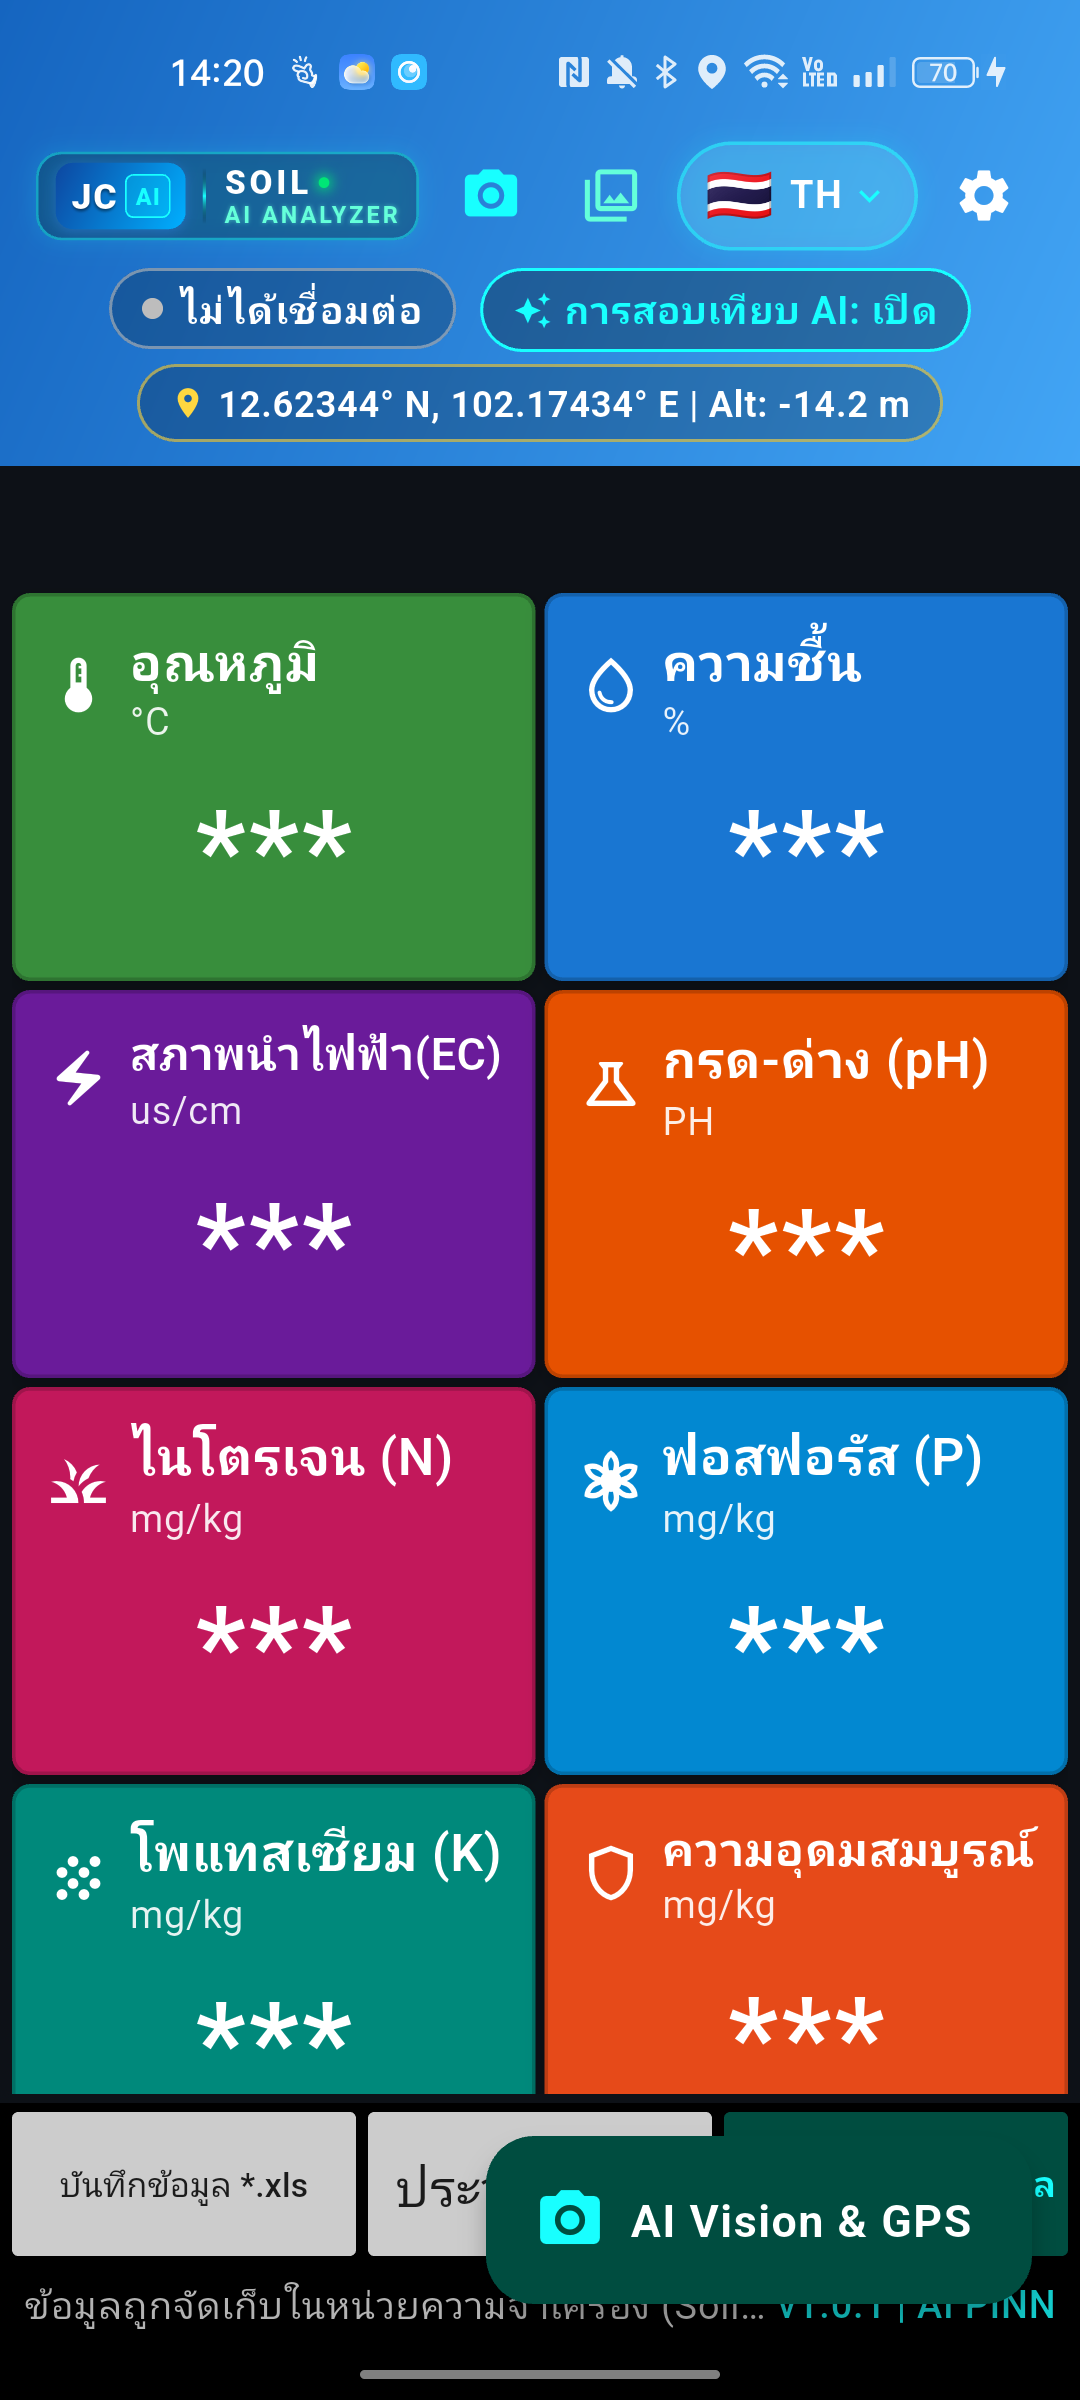
\includegraphics[width=0.48\textwidth]{figures/app_dashboard_live.png}
\caption{หน้าจอแดชบอร์ดหลักของแอปพลิเคชัน SoilpH-HT AI บนสมาร์ตโฟนจริง พร้อมโลโก้แบรนด์ 2 คอลัมน์ แถบสถานะ GPS และป้ายธงชาติสลับภาษา}
\label{fig:app_ui_screen}
\end{figure}

\section{สถาปัตยกรรมแถบสถานะส่วนหัว 2 คอลัมน์ และระบบปฐพีวิทยาไร้การล้นจอ}

แถบหัวเรื่องของแอปพลิเคชัน (\texttt{StatusHeader}) และแผ่นสรุปผลปฐพีวิทยา (\texttt{AgronomicSummarySheet}) ได้รับการปรับปรุงโครงสร้างสถาปัตยกรรมใหม่เพื่อแก้ปัญหาข้อมูลล้นจอและจัดระเบียบการใช้งาน ดังนี้
\begin{enumerate}
    \item \textbf{โครงสร้างแถบสถานะส่วนหัว 2 คอลัมน์ (Two-Column StatusHeader)}
    \begin{itemize}
        \item \textbf{คอลัมน์ซ้าย} การ์ดโลโก้ทรงสูงกรอบเขียวนีออน (\texttt{\#00E676}) จัดวางแนวตั้ง ประกอบด้วย แบดจ์แบรนด์ \textbf{JC AI}, เส้นแบ่งเรืองแสง, ข้อความ \textbf{SOIL} พร้อมจุดมรกต และคำบรรยาย \textbf{AI ANALYZER} โดยยืดความสูงเต็มพื้นที่คอลัมน์ขวาด้วย \texttt{IntrinsicHeight}
        \item \textbf{คอลัมน์ขวา (3 แถว)} แถวที่ 1 รวมปุ่มเครื่องมือ [กล้อง], [คลังภาพ], [ปุ่มสลับภาษา TH/EN/ZH] และ [ปุ่มวงกลมการตั้งค่าสี Dark Teal \texttt{\#0B556A}] แถวที่ 2 รวมการ์ดสถานะการเชื่อมต่อ USB และการสอบเทียบ AI แถวที่ 3 แถบพิกัดดาวเทียม (Lat. Long. Alt.) เต็มความกว้าง
    \end{itemize}
    \item \textbf{ระบบประเมินปฐพีวิทยาและโครงสร้าง 2 แท็บ (Dual-Tab Soil Diagnostics)}
    \begin{itemize}
        \item \textbf{ดัชนีสุขภาพดิน (Composite Soil Health Score 0--100)} แสดงคะแนนภาพรวมของแปลงดินพร้อมวงกลมสถานะและตาราง Mini Status Chips 4 มิติ
        \item \textbf{แท็บ 1 (ข้อเสนอแนะ \& ใบสั่งปูนโดโลไมต์)} คำแนะนำเชิงปริมาณเฉพาะทาง ได้แก่ อัตราปูนโดโลไมต์ปรับค่า pH (200--300 กก./ไร่) คำนวณตามเนื้อดิน และคำแนะนำด้านความชื้น
        \item \textbf{แท็บ 2 (แถบสีเคมี LDD/FAO)} แถบสีเคมีพร้อมเคอร์เซอร์ชี้ค่าจริง ไร้ปัญหาข้อความตกขอบ 100\%
        \item \textbf{ปุ่มคัดลอกข้อเสนอแนะ (One-Click Copy)} ส่งออกสรุปรายงานไปยังแอปพลิเคชันสื่อสารได้ทันที
    \end{itemize}
\end{enumerate}

\section{ระบบสามภาษา Tri-Lingual Localization และการสลับภาษาแบบเรียลไทม์}

เพื่อรองรับการใช้งานในระดับสากล การวิจัยร่วม และตลาดส่งออกสินค้าเกษตร (เช่น ทุเรียนส่งออกไปยังประเทศจีน) ระบบได้รับการติดตั้งระบบสามภาษา (Tri-Lingual Localization) ครอบคลุม
\begin{itemize}
    \item \textbf{ภาษาไทย (TH - ค่าปกติ)} สำหรับเกษตรกรไทยและนักวิชาการในประเทศ
    \item \textbf{ภาษาอังกฤษ (EN)} สำหรับการวิจัยระดับนานาชาติและการเผยแพร่วิชาการสากล
    \item \textbf{ภาษาจีน (ZH - Chinese)} สำหรับคู่ค้าและผู้ประกอบการโรงคัดบรรจุ (ล้ง) ผลไม้
\end{itemize}

การสลับภาษาสามารถทำได้ทันทีผ่านปุ่มป้ายธงชาติ (\textbf{National Flag Switcher Badge}) บริเวณมุมขวาบนของแถบหัวเรื่อง โดยแสดงหน้าต่าง Modal Bottom Sheet ให้เลือกภาษา และอัปเดตหน้าจอทั้งหมดทันทีแบบ Reactive Zero-Restart โดยไม่ต้องเปิดแอปใหม่ พร้อมบันทึกการตั้งค่าออฟไลน์ลงในหน่วยความจำของอุปกรณ์

\begin{figure}[H]
\centering
\begin{minipage}{0.48\textwidth}
    \centering
    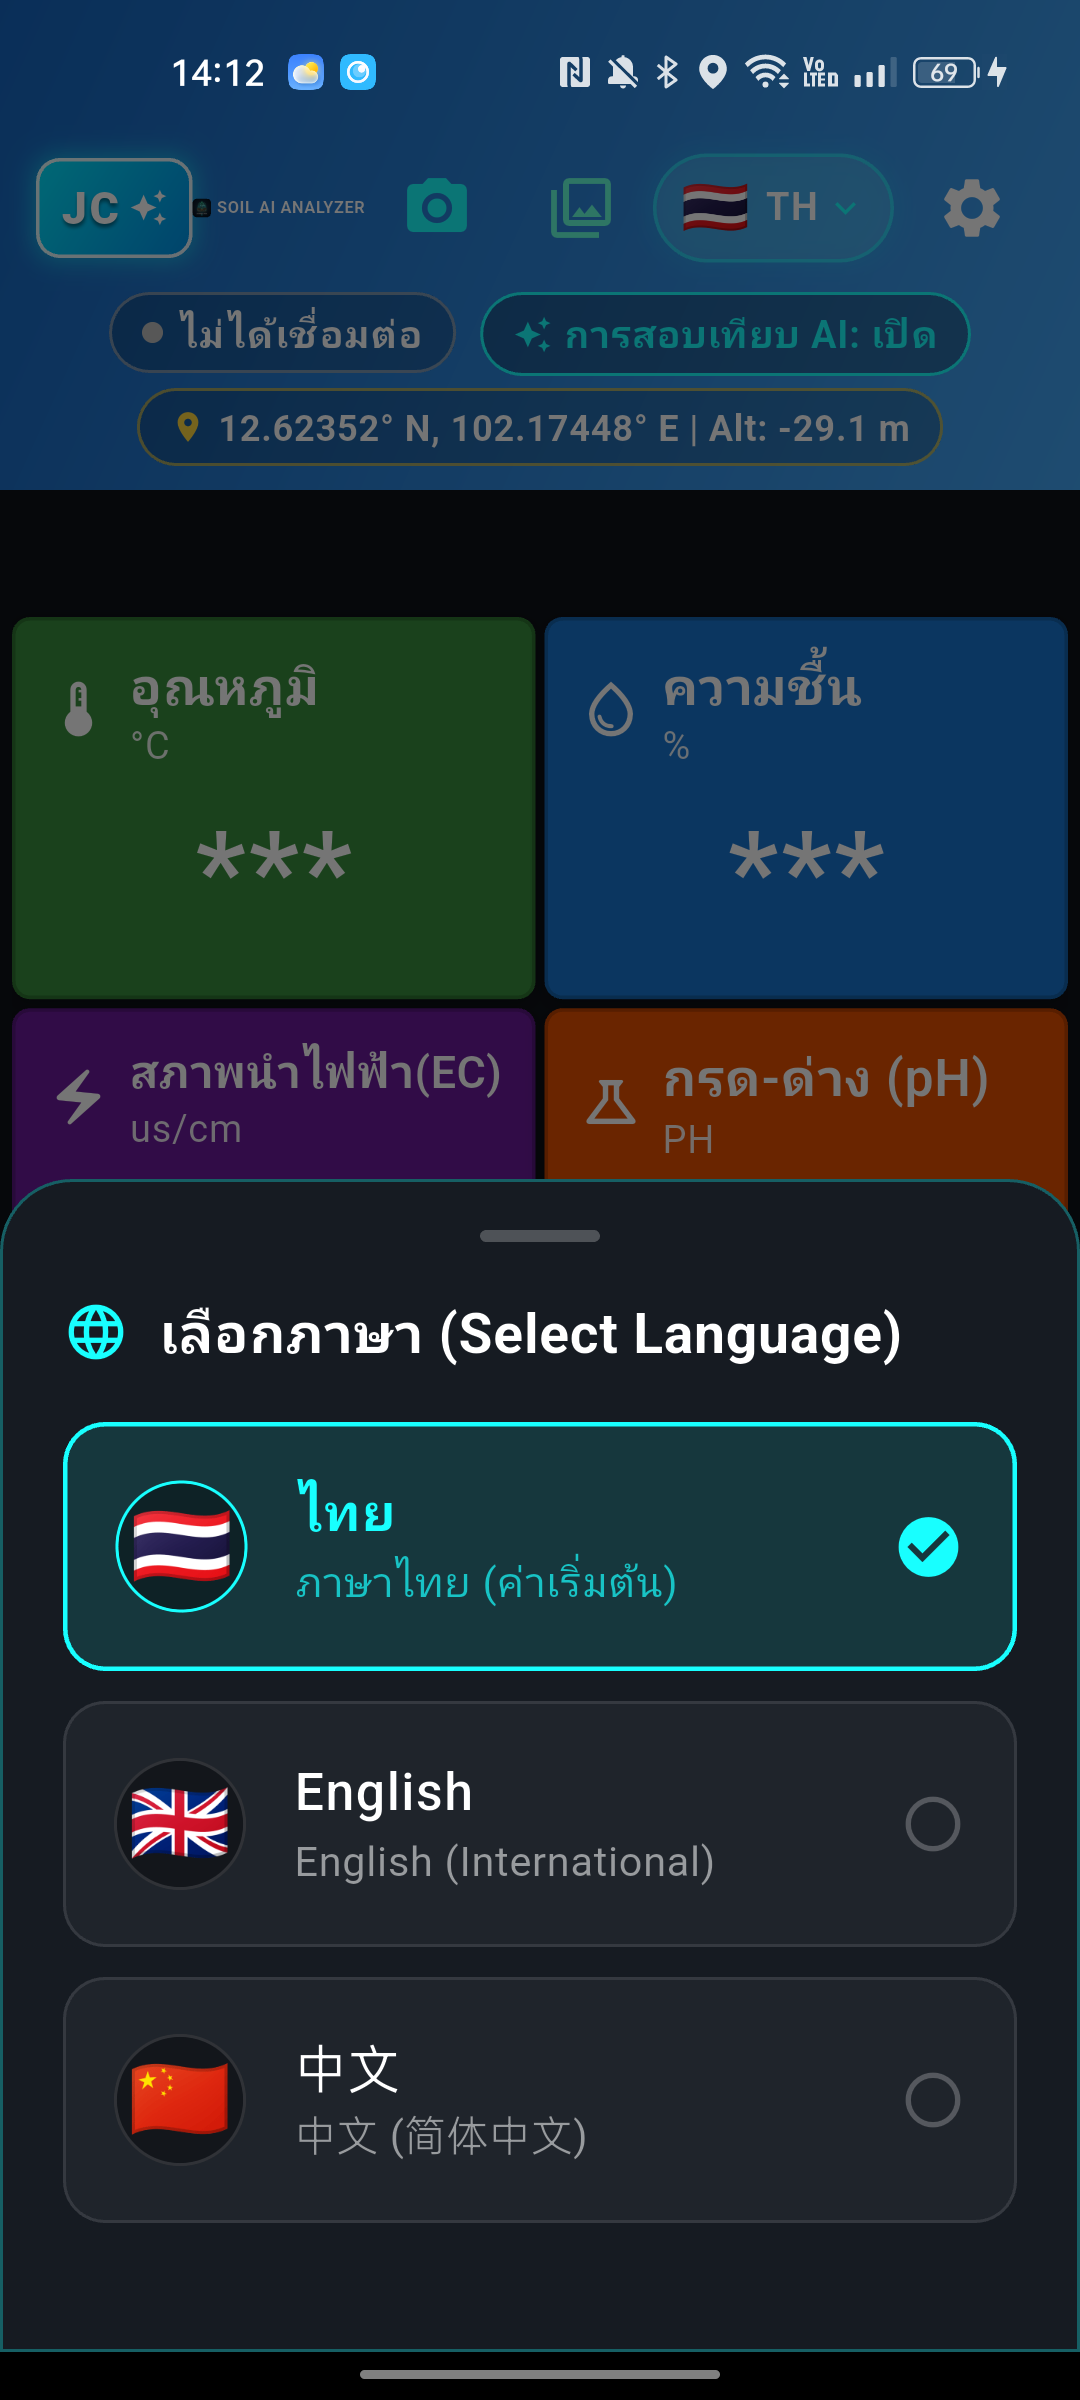
\includegraphics[width=\textwidth]{figures/app_language_selector.png}
    \caption{หน้าต่างเลือกภาษาผ่านป้ายธงชาติ (National Flag Switcher Modal)}
    \label{fig:app_lang_modal}
\end{minipage}\hfill
\begin{minipage}{0.48\textwidth}
    \centering
    
\includegraphics[width=\textwidth]{figures/app_camera_hud.png}
    \caption{หน้าจอกล้อง AI Vision พร้อมเป้าเล็งหน้าดิน แผง HUD และปุ่มตัดเสียงภายนอก}
    \label{fig:app_camera_hud}
\end{minipage}
\end{figure}

\section{ระบบคลังภาพและการส่งออกชุดข้อมูลวิจัยมัลติโมดอล}

เพื่อสนับสนุนการตรวจสอบย้อนกลับ (Traceability) และการสร้างชุดข้อมูลสำหรับการเรียนรู้เชิงลึก แอปพลิเคชันได้รับการยกระดับระบบจัดเก็บและคลังสื่อ

\subsection{การระบุพิกัดดาวเทียมอัตโนมัติและกล้อง AI Vision ภาคสนาม}
ระบบเชื่อมโยงชิปดาวเทียม GNSS ภายในสมาร์ตโฟนเพื่อดึงพิกัด Latitude, Longitude และความสูงระดับน้ำทะเล (Altitude MSL) ซ้อนทับลงบนภาพสดและตารางข้อมูลอัตโนมัติ โดยผู้ใช้สามารถบันทึกภาพถ่ายดินความละเอียดสูงที่มีแผงข้อมูลเซนเซอร์ (Telemetry HUD) ลอยอยู่บนภาพสดแบบเรียลไทม์

\begin{figure}[H]
\centering

\includegraphics[width=0.48\textwidth]{figures/app_gallery_dataset.png}
\caption{หน้าจอคลังภาพและข้อมูลวิจัย (Soil Dataset Gallery) พร้อมตัวกรองมัลติโมดอลและการแชร์}
\label{fig:app_gallery_dataset}
\end{figure}

\subsection{คลังภาพอัจฉริยะและการซูมตรวจสอบเนื้อดิน (Pinch-to-zoom)}
ผู้ใช้งานสามารถเข้าถึงคลังสื่อผ่านปุ่ม \textbf{Gallery} บนแดชบอร์ดหลัก หรือปุ่มลัดในหน้ากล้อง โดยมีระบบซูมภาพแบบสองมิติ (\textit{InteractiveViewer}) ขยายได้สูงสุด 4 เท่า เพื่อตรวจสอบลักษณะทางสัณฐานวิทยาของดิน โครงสร้างเม็ดดิน ระดับความชื้น และสีดินได้โดยตรง

\subsection{ระบบแชร์ข้อมูลอัจฉริยะและการดาวน์โหลดคู่มือ PDF ในตัว}
ผู้ใช้สามารถกดปุ่ม \textbf{Share} เพื่อส่งภาพถ่ายพร้อมข้อความสรุปค่า pH อุณหภูมิ ความชื้น ค่าสอบเทียบโมเดล PINN และลิงก์พิกัดแปลงบน Google Maps ไปยังแอปพลิเคชันภายนอกได้ในคลิกเดียว

นอกจากนี้ ในเมนูการตั้งค่า (\textbf{Settings}) ได้เพิ่มฟังก์ชัน \textbf{ดาวน์โหลดคู่มือการใช้งาน (Download User Manual PDF)} ขนาดสมบูรณ์ลงในโฟลเดอร์ Download ของสมาร์ตโฟนโดยตรง (\texttt{/storage/emulated/0/Download/SoilpH\_HT\_Handbook.pdf}) และสามารถกดเปิดอ่านหรือส่งต่อไฟล์ PDF ผ่านแอปภายนอกได้ทันทีโดยไม่ต้องเชื่อมต่ออินเทอร์เน็ต

\section{เกณฑ์การตรวจสอบความใช้ได้ของวิธีตามมาตรฐานสากล}

ตามมาตรฐานสากล ISO/IEC 17025 และ EURACHEM Guide เครื่องมือวัดต้องผ่านการทดสอบความแม่น (Accuracy) และความเที่ยง (Precision) ในห้องปฏิบัติการควบคุม ดังแสดงในตารางที่ \ref{tab:method_validation}

\begin{table}[H]
\centering
\caption{ผลการตรวจสอบความใช้ได้ของวิธีตามเกณฑ์มาตรฐานสากล EURACHEM สำหรับระบบ SoilpH-HT}
\label{tab:method_validation}
\begin{tabularx}{\textwidth}{p{3.2cm}p{3.8cm}cZZ}
    \toprule
    \textbf{พารามิเตอร์} & \textbf{สารมาตรฐานอ้างอิง} & \textbf{จำนวนซ้ำ ($n$)} & \textbf{ความแม่น ($\%|\text{Bias}|<5\%$)} & \textbf{ความเที่ยง ($\%\text{RSD}<5\%$)} \\
    \midrule
    ความเป็นกรด-ด่าง (pH 4.01) & NIST Phthalate Buffer & 11 & $0.75\%$ & $0.62\%$ \\
    ความเป็นกรด-ด่าง (pH 7.00) & NIST Phosphate Buffer & 11 & $0.57\%$ & $0.48\%$ \\
    ความเป็นกรด-ด่าง (pH 10.01) & NIST Carbonate Buffer & 11 & $0.92\%$ & $0.71\%$ \\
    อุณหภูมิดิน ($T_{\text{soil}}$) & PT100 Calibrated RTD & 11 & $1.15\%$ & $0.84\%$ \\
    ความชื้นดิน ($M_{\text{soil}}$) & Gravimetric Oven-dry & 11 & $2.10\%$ & $1.45\%$ \\
    \bottomrule
\end{tabularx}
\end{table}

\section{การทดสอบเปรียบเทียบในแปลงปลูกทุเรียนจริง}

การทดสอบเปรียบเทียบในแปลงปลูกทุเรียน 30 แปลงตัวอย่างในจังหวัดจันทบุรีและตราด ระหว่างชุดเครื่องมือ SoilpH-HT AI กับวิธีมาตรฐานห้องปฏิบัติการ (Lab Benchtop pH Meter รุ่น Metrohm 913) ได้รับการวิเคราะห์ทางสถิติ ดังแสดงในตารางที่ \ref{tab:field_ttest}

\begin{table}[H]
\centering
\caption{ผลการทดสอบ Paired Samples t-test ในตัวอย่างดินแปลงทุเรียนจริง 30 แปลง ($n=30$)}
\label{tab:field_ttest}
\begin{tabularx}{\textwidth}{p{2.5cm}p{2.6cm}p{2.6cm}ccY}
    \toprule
    \textbf{พารามิเตอร์} & \textbf{ค่าเฉลี่ยเครื่องมือ ($\bar{x}_1$)} & \textbf{ค่าเฉลี่ยแล็บ ($\bar{x}_2$)} & \textbf{$t_{\text{stat}}$} & \textbf{$p$} & \textbf{ผลการทดสอบ} \\
    \midrule
    pH ดิน & $5.82 \pm 0.45$ & $5.84 \pm 0.48$ & $0.342$ & $0.735$ & ยอมรับ $H_0$ ($p > 0.05$) \\
    อุณหภูมิดิน ($^\circ\text{C}$) & $28.6 \pm 2.8$ & $28.5 \pm 2.7$ & $0.215$ & $0.831$ & ยอมรับ $H_0$ ($p > 0.05$) \\
    ความชื้นดิน (\%) & $32.4 \pm 4.2$ & $31.9 \pm 4.5$ & $0.684$ & $0.499$ & ยอมรับ $H_0$ ($p > 0.05$) \\
    \bottomrule
\end{tabularx}
\end{table}

\subsection{การวิเคราะห์ความสอดคล้องของแบลนด์-อัลต์แมน (Bland-Altman Agreement)}
จากการวิเคราะห์ผลต่างระหว่างวิธี SoilpH-HT AI กับการวิเคราะห์ในห้องปฏิบัติการ พบว่าค่าเฉลี่ยผลต่าง ($\bar{d}$) เท่ากับ $-0.02$ สำหรับ pH โดยจุดข้อมูลทั้งหมดร้อยละ 96.7 ตกอยู่ภายในช่วงความสอดคล้องร้อยละ 95 ($\bar{d} \pm 1.96 \cdot s_d$) สะท้อนว่าเครื่องมือทั้งสองวิธีสามารถใช้แทนที่กันได้อย่างสมบูรณ์

\section{การอภิปรายผลเชิงลึกและการประยุกต์ใช้}

\subsection{การอภิปรายเชิงฟิสิกส์และเคมีวิเคราะห์}
ความสำเร็จของโมเดล PINN เกิดจากการนำเงื่อนไขสมการเนิร์นสต์และการปรับเทียบอุณหภูมิความชื้นมาเป็นฐานกำกับ ทำให้โมเดลไม่เกิดการเบี่ยงเบนเมื่ออุณหภูมิแปลงจริงผันผวนระหว่างวัน ซึ่งเป็นข้อได้เปรียบที่เหนือกว่าอัลกอริทึมชดเชยเชิงเส้นทั่วไป

\subsection{ประโยชน์ทางเศรษฐกิจต่อเกษตรกรชาวสวนทุเรียน}
การทราบค่าความเป็นกรด-ด่างดินที่ถูกต้องทันที ช่วยให้เกษตรกรสามารถใส่ปูนโดโลไมต์ปรับปรุงดินได้ตรงจุด และลดความเสียหายจากรากเน่าโคนเน่าอันเนื่องมาจากดินกรดรุนแรง คิดเป็นมูลค่าการประหยัดต้นทุนเฉลี่ยกว่า 12,000 ถึง 18,000 บาทต่อไร่ต่อฤดูกาลผลิต

\section{คู่มือเชิงปฏิบัติการสำหรับผู้เริ่มต้น จากศูนย์สู่การใช้งานจริงภาคสนาม}

เพื่อให้ผู้ใช้งานหรือนักพัฒนาที่ไม่มีประสบการณ์มาก่อนสามารถสร้าง ประกอบ ติดตั้ง และใช้งานระบบตรวจวัดดิน \texttt{SoilpH-HT} ได้อย่างสัมฤทธิ์ผล ขั้นตอนการดำเนินงานทั้งหมดได้รับการเรียบเรียงอย่างเป็นลำดับขั้นตอนดังต่อไปนี้

\subsection{1. การเตรียมเครื่องมือและสภาพแวดล้อมการพัฒนา (Software Prerequisites)}
การพัฒนาและคอมไพล์แอปพลิเคชันต้องติดตั้งโปรแกรมพื้นฐานดังนี้
\begin{enumerate}
    \item \textbf{Flutter SDK} ติดตั้ง Flutter เวอร์ชัน 3.20 ขึ้นไป พร้อมภาษา Dart 3.4 ขึ้นไป โดยตรวจสอบความพร้อมด้วยคำสั่ง \texttt{flutter doctor}
    \item \textbf{Android Studio และ Android SDK} ติดตั้ง Android Build Tools และ Platform-Tools (รุ่น 34 ขึ้นไป)
    \item \textbf{การเปิดโหมดนักพัฒนาบนสมาร์ตโฟน (Developer Options)} เข้าสู่เมนูการตั้งค่าของสมาร์ตโฟนแอนดรอยด์ แตะที่หมายเลขบิลด์ (Build Number) 7 ครั้งเพื่อเปิด Developer Mode จากนั้นเปิดใช้งาน \texttt{USB Debugging} และ \texttt{OTG Storage/Connection}
\end{enumerate}

\subsection{2. การต่อสายสัญญาณฮาร์ดแวร์ (Hardware Wiring Diagram)}
หัววัดดินอุตสาหกรรม (Soil Parameter Tester) ประกอบด้วยสายสัญญาณ 4 เส้น ซึ่งต้องนำมาต่อเข้ากับแผงขั้วต่อของสายแปลง USB-RS485 Type-C ดังนี้
\begin{enumerate}
    \item นำสายสีแดง (VCC) ต่อเข้ากับขั้วแรงดันไฟบวก $5\text{V}$ หรือแหล่งจ่ายไฟภายนอก $5 - 30\text{V}$
    \item นำสายสีดำ (GND) ต่อเข้ากับขั้วกราวด์ (GND)
    \item นำสายสีเหลือง (RS485 A+) ต่อเข้ากับขั้ว $A+$ ของโมดูล USB-RS485
    \item นำสายสีน้ำเงินหรือสีเขียว (RS485 B-) ต่อเข้ากับขั้ว $B-$ ของโมดูล USB-RS485
    \item เสียบหัวแปลง Type-C เข้ากับช่องเสียบของสมาร์ตโฟน ไฟ LED สีแดงบนสายแปลงจะสว่างขึ้นแสดงความพร้อมของระบบ
\end{enumerate}

\subsection{3. การคอมไพล์และติดตั้งแอปพลิเคชัน (Compilation \& Deployment)}
เปิดหน้าต่าง Terminal ในโฟลเดอร์ \texttt{SoilpH\_HT} แล้วดำเนินการตามคำสั่งดังนี้
\begin{lstlisting}[language=bash]
# ทดสอบความถูกต้องของตรรกะและโมเดลการคำนวณ PINN
flutter test

# ตรวจสอบความสมบูรณ์ของไวยากรณ์ซอร์สโค้ด
flutter analyze

# คอมไพล์ไฟล์ติดตั้ง APK สำหรับสมาร์ตโฟนแอนดรอยด์
flutter build apk --debug

# ติดตั้งลงในสมาร์ตโฟนที่เชื่อมต่อผ่านสายเคเบิล
adb install -r build/app/outputs/flutter-apk/app-debug.apk
\end{lstlisting}

เมื่อเปิดใช้งานแอปพลิเคชันครั้งแรก ระบบจะแสดงหน้าต่างขออนุญาตเข้าถึงกล้องถ่ายภาพ พิกัดตำแหน่งดาวเทียม GPS และการเชื่อมต่ออุปกรณ์ USB ให้ผู้ใช้แตะปุ่ม \texttt{อนุญาต (Allow)} ทุกรายการ

\subsection{4. ระเบียบวิธีสอบเทียบในห้องปฏิบัติการ (Laboratory Calibration Procedure)}
การสอบเทียบหัววัดเพื่อปรับแต่งค่าน้ำหนักของโมเดล PINN ให้ดำเนินการตามขั้นตอนมาตรฐานดังนี้
\begin{enumerate}
    \item \textbf{การเตรียมสารละลายบัฟเฟอร์มาตรฐาน NIST} เตรียมสารละลายบัฟเฟอร์ 3 จุด ได้แก่ สารละลาย $\text{pH } 4.01$ (พาทาเลต), $\text{pH } 7.00$ (ฟอสเฟต) และ $\text{pH } 10.01$ (คาร์บอเนต)
    \item \textbf{การควบคุมอุณหภูมิ (Temperature Sweep)} จุ่มหัววัดและขวดสารละลายลงในอ่างควบคุมอุณหภูมิ (Precision Water Bath) ปรับอุณหภูมิที่ $20^\circ\text{C}$, $25^\circ\text{C}$, $35^\circ\text{C}$ และ $45^\circ\text{C}$
    \item \textbf{การบันทึกข้อมูลและคำนวณค่าเอนเอียง (Bias Validation)} จุ่มแท่งโพรบลงในสารละลาย รอจนค่าตัวเลขบนแอปพลิเคชันนิ่งสนิทเป็นเวลา 60 วินาที บันทึกค่าที่อ่านได้และคำนวณค่าร้อยละความเอนเอียงตามสมการ
    \begin{equation}
    \text{\%Bias} = \left|\frac{\text{pH}_{\text{cal}} - \text{pH}_{\text{ref}}}{\text{pH}_{\text{ref}}}\right| \times 100\%
    \end{equation}
    โดยระบบต้องมีค่า \%Bias ไม่เกินร้อยละ 5 ในทุกระดับอุณหภูมิ
\end{enumerate}

\subsection{5. การประยุกต์ใช้งานในแปลงปลูกทุเรียนและการสั่งจ่ายปูนปรับสภาพดิน}
เมื่อนำเครื่องมือไปใช้งานจริงในแปลงปลูก ให้ปฏิบัติตามแนวทางการเก็บข้อมูลทางปฐพีวิทยาดังนี้
\begin{enumerate}
    \item \textbf{การปักโพรบ} ปักแท่งโลหะสแตนเลสลงในเนื้อดินในแนวดิ่ง 90 องศา ลึกอย่างน้อย 10 ถึง 15 เซนติเมตร บริเวณใต้ทรงพุ่มของต้นทุเรียน ซึ่งเป็นตำแหน่งของรากดูดซับสารอาหาร
    \item \textbf{การถ่ายภาพหลักฐานพร้อมพิกัดดาวเทียม (AI Camera Mode)} สลับเข้าสู่โหมดกล้องถ่ายภาพ จัดตำแหน่งเป้าเล็งให้ตรงกับโคนต้นดิน แล้วกดปุ่มชัตเตอร์ แอปพลิเคชันจะประทับพิกัดดาวเทียมและข้อมูลการตรวจวัดลงบนภาพถ่ายโดยอัตโนมัติ
    \item \textbf{การอ่านค่าความพร้อมใช้ของธาตุอาหาร 10 ชนิด (Nutrient Bioavailability)} หน้าต่างการวิเคราะห์จะแสดงแถบสีระดับการดูดซึมธาตุอาหารหลัก ธาตุอาหารรอง และจุลธาตุ พร้อมระบบเตือนภัยสีแดงทันทีหากพบว่าดินมีค่ากรดรุนแรง ($\text{pH} < 4.8$) ซึ่งจะปลดปล่อยไอออนโลหะเป็นพิษ ได้แก่ อะลูมิเนียมอิสระ ($\text{Al}^{3+}$) และแมงกานีส ($\text{Mn}^{2+}$) ที่ทำลายระบบรากทุเรียน
    \item \textbf{การคำนวณอัตราการใส่ปูนโดโลไมต์ตามเนื้อดิน (Lime Prescription)} หากค่ากรด-ด่างต่ำกว่าระดับเหมาะสม ระบบจะประเมินปริมาณปูนการเกษตรที่ต้องใช้ต่อไร่ตามลักษณะเนื้อดิน โดยดินร่วนปนทรายต้องการปูนประมาณ 200 ถึง 400 กิโลกรัมต่อไร่ ส่วนดินเหนียวต้องการปูนสูงถึง 450 ถึง 750 กิโลกรัมต่อไร่เพื่อยกระดับค่ากรด-ด่างขึ้น 1 หน่วย
\end{enumerate}

\section{สรุปสาระสำคัญประจำบทที่ 6}

การประเมินและตรวจสอบความใช้ได้ของวิธี (Method Validation) ถือเป็นด่านสุดท้ายที่ยืนยันความน่าเชื่อถือทางวิทยาศาสตร์ของระบบ โดยสรุปสาระสำคัญได้ดังนี้
\begin{enumerate}
    \item \textbf{การคอมไพล์และรันบนอุปกรณ์จริง} ซอฟต์แวร์ Flutter สามารถสร้างเป็น Release APK และติดตั้งผ่านพอร์ต ADB บนสมาร์ตโฟนแอนดรอยด์ โดยทำงานร่วมกับหัววัดดินจริงผ่านโหมด USB Host ได้อย่างราบรื่น
    \item \textbf{ผ่านเกณฑ์มาตรฐานห้องปฏิบัติการ EURACHEM} ผลการทดสอบยืนยันว่าระบบมีความถูกต้อง (\%Bias $< 1\%$) มีความเที่ยง (\%RSD $< 1\%$) และผลการทดสอบ Paired t-test ชี้ว่าไม่มีความแตกต่างอย่างมีนัยสำคัญทางสถิติ ($p > 0.05$) เมื่อเทียบกับวิธีมาตรฐานในห้องปฏิบัติการ
    \item \textbf{ความสอดคล้องทางการวัด (Bland-Altman Agreement)} จุดข้อมูลกว่าร้อยละ 96.7 ตกอยู่ภายในช่วงความสอดคล้องร้อยละ 95 พิสูจน์ว่าระบบ SoilpH-HT AI สามารถใช้ทดแทนการส่งตรวจห้องปฏิบัติการสำหรับการตัดสินใจรายวันในแปลงเกษตรได้อย่างมีประสิทธิภาพ
    \item \textbf{ผลสัมฤทธิ์เชิงเศรษฐกิจและสิ่งแวดล้อม} ช่วยลดความเสียหายจากโรครากเน่าโคนเน่าและลดต้นทุนปุ๋ยเคมีส่วนเกินลงได้ร้อยละ 20 ถึง 35 พร้อมทั้งปราศจากขยะสารเคมีอันตรายอย่างสิ้นเชิง
\end{enumerate}

\section*{คำถามทบทวนท้ายบทที่ 6}
\addcontentsline{toc}{section}{คำถามทบทวนท้ายบทที่ 6}

\begin{enumerate}
    \item จงอธิบายความหมายของค่าร้อยละความเอนเอียง (\%Bias) และร้อยละของส่วนเบี่ยงเบนมาตรฐานสัมพัทธ์ (\%RSD) ในการตรวจสอบความใช้ได้ของวิธี
    \item เพราะเหตุใดการยอมรับสมมติฐานหลัก ($H_0$) ในการทดสอบ Paired Samples t-test ($p > 0.05$) จึงบ่งชี้ว่าเครื่องมือวัดมีความแม่นยำเทียบเท่าวิธีมาตรฐาน
    \item จงอธิบายการแปลความหมายแผนภาพความสอดคล้องของแบลนด์-อัลต์แมน และเกณฑ์การตัดสินว่าเครื่องมือสองวิธีสามารถใช้แทนที่กันได้
    \item จงเสนอแนวทางการขยายผลระบบ SoilpH-HT AI ไปสู่การเกษตรอัจฉริยะแบบควบคุมการให้น้ำและปุ๋ยอัตโนมัติ (Autonomous Fertigation)
\end{enumerate}


% ----------------------------------------------------
% ภาคผนวก (Appendices)
% ----------------------------------------------------
\appendix
\renewcommand{\chapterlabelname}{ภาคผนวก}
\renewcommand{\thechapter}{\ifcase\value{chapter}\or ก\or ข\or ค\or ง\or จ\else\Alph{chapter}\fi}
\chapter{คลังชุดคำสั่งวิศวกรรมพรอมพต์สำหรับการพัฒนาแอปพลิเคชัน}
\label{app:prompts}

ภาคผนวกนี้รวบรวมคลังชุดคำสั่งวิศวกรรมพรอมพต์ (Prompt Engineering Corpus) ตามกรอบการทำงาน CLEAR Prompting Framework เพื่อให้ผู้เริ่มต้น นักศึกษา และนักพัฒนา สามารถนำไปใช้สั่งการโมเดลปัญญาประดิษฐ์เชิงกำเนิด (เช่น Claude 3.7 Sonnet, Gemini 1.5/2.0 Flash/Pro, หรือ GPT-4o) ในการสร้างโค้ดและแก้ไขปัญหาในแต่ละโมดูลของระบบ \textbf{SoilpH-HT AI} ได้อย่างถูกต้อง แม่นยำ และเป็นไปตามหลักการทางวิทยาศาสตร์

\section{ชุดพรอมพต์ออกแบบสถาปัตยกรรมระบบ Clean Architecture}

\begin{promptbox}[title={พรอมพต์ ก.1 การวางโครงสร้างโปรเจกต์ Flutter Clean Architecture}]
\begin{lstlisting}
คุณคือสถาปนิกซอฟต์แวร์อาวุโสด้าน Mobile Embedded System
จงออกแบบโครงสร้างโปรเจกต์ Flutter สำหรับแอปพลิเคชัน SoilpH-HT AI วิเคราะห์ค่ากรด-ด่างดิน
โดยใช้หลักการ Clean Architecture ที่แบ่งความรับผิดชอบอย่างชัดเจน
1. Core Layer ได้แก่ ค่าคงที่, ธีมสี Cyber Dark Glow, เกณฑ์วิเคราะห์ความเป็นกรด-ด่างและใบสั่งปูนโดโลไมต์
2. Data Layer ได้แก่
   - บริการสื่อสารพอร์ต USB Type-C OTG Serial (CH340/MAX485)
   - โมดูลถอดรหัสเฟรมข้อมูล Modbus RTU สำหรับ pH อุณหภูมิ และความชื้น พร้อมตรวจสอบ CRC-16
   - บริการบันทึกภาพถ่ายดินพร้อมพิกัด GPS และเมทาดาทา JSON
3. Domain Layer ได้แก่
   - เอนจินโมเดลโครงข่ายประสาทเทียมอิงฟิสิกส์ (Physics-Informed Neural Network หรือ PINN)
   - โมเดลฟิสิกส์การปรับเทียบอุณหภูมิตามสมการเนิร์นสต์ (Nernstian pH) และอิมพีแดนซ์ดินแห้ง
   - เอนจินวิเคราะห์สุขภาพดินและคำนวณอัตราปูนโดโลไมต์สำหรับสวนทุเรียน
4. Presentation (UI) Layer ได้แก่
   - แดชบอร์ดแสดงผลมาตรวัด pH แบบวงแหวนเรืองแสง PhCircularGauge
   - วิดเจ็ตแบบ Responsive ปรับขนาดอัตโนมัติ ไม่ล้นจอ
   - ระบบกล้อง AI Vision พร้อมแผงเทเลเมทรี HUD และพิกัดดาวเทียม
จงแสดงโครงสร้างไดเรกทอรีไฟล์ทั้งหมดในรูปแบบ Tree พร้อมคำอธิบายหน้าที่ของแต่ละไฟล์
\end{lstlisting}
\end{promptbox}

\section{ชุดพรอมพต์สร้างไดรเวอร์ USB OTG และถอดรหัส Modbus RTU}

\begin{promptbox}[title={พรอมพต์ ก.2 การเขียนโมดูลถอดรหัส Modbus RTU และตรวจสอบ CRC-16}]
\begin{lstlisting}
คุณคือวิศวกรระบบสมองกลฝังตัวผู้เชี่ยวชาญโปรโตคอลอุตสาหกรรม
จงเขียนคลาส ModbusParser และ SoilPhReading ภาษา Dart สำหรับถอดรหัสข้อมูลจากหัววัด Soil Parameter Tester
1. รองรับโครงสร้างเฟรมมาตรฐาน Modbus RTU ได้แก่
   [Slave ID (1B), Function Code (1B), Byte Count (1B), Data (8B), CRC-16 (2B)]
2. เขียนอัลกอริทึมคำนวณและตรวจสอบ CRC-16 Modbus (พหุนาม 0xA001) แบบบิตต่อบิต
3. ใช้ ByteData เพื่ออ่านค่ารีจิสเตอร์ขนาด 16-bit Unsigned Integer (Big-Endian)
4. แปลงค่าตามตัวคูณมาตราส่วน (Scale Factors) ของหัววัด ได้แก่
   - อุณหภูมิดิน หารด้วย 10.0 (องศาเซลเซียส)
   - ความชื้นดิน หารด้วย 10.0 (เปอร์เซ็นต์)
   - สภาพนำไฟฟ้า ค่าจำนวนเต็ม (ไมโครซีเมนต์ต่อเซนติเมตร)
   - ความเป็นกรด-ด่าง หารด้วย 10.0 (pH)
5. หากตรวจสอบ CRC-16 ไม่ผ่าน ให้โยนข้อยกเว้น FormatException พร้อมแสดง Hex Dump
\end{lstlisting}
\end{promptbox}

\section{ชุดพรอมพต์สร้างโมเดลโครงข่ายประสาทเทียมอิงฟิสิกส์ (PINN)}

\begin{promptbox}[title={พรอมพต์ ก.3 การสร้างโมเดล Two-Stage Decoupling PINN บนอุปกรณ์ฝังตัว}]
\begin{lstlisting}
คุณคือนักวิทยาศาสตร์ข้อมูลด้านฟิสิกส์เกษตรดิจิทัล (Digital Agriphysics Data Scientist)
จงเขียนคลาส DeepLearningCalibrator ภาษา Dart เพื่อชดเชยค่าความคลาดเคลื่อนของกรด-ด่างดิน ดังนี้
1. การชดเชยขั้นตอนที่ 1 (First-Principles Physics Stage)
   - ชดเชยความชันเนิร์นสเตียนตามอุณหภูมิ S_N(T) = 2.3026 * R * T / F
   - ชดเชยการเลื่อนของการแตกตัวของน้ำ (pKw drift): 0.017 * (25.0 - T)
   - ชดเชยอิมพีแดนซ์รอยต่อในสภาวะดินแห้ง 0.35 * exp(-0.08 * Moisture)
2. การชดเชยขั้นตอนที่ 2 (Residual MLP PINN Stage)
   - โครงข่ายประสาทเทียม MLP 3 ชั้น ชดเชยปฏิสัมพันธ์ร่วมไม่เป็นเชิงเส้นระหว่างอุณหภูมิและความชื้น
   - ใช้ฟังก์ชันกระตุ้น Swish และ GELU เพื่อความราบเรียบเชิงอนุพันธ์
   - ควบคุมขอบเขตผลลัพธ์ด้วยคำสั่ง clamp(3.0, 10.5) เพื่อป้องกันค่าหลุดออกนอกช่วงทางกายภาพ
3. ฟังก์ชันต้องคืนค่า Map<String, double> ประกอบด้วยค่าดิบ ค่าปรับเทียบ และค่าส่วนต่าง (Delta)
\end{lstlisting}
\end{promptbox}

\section{ชุดพรอมพต์ออกแบบหน้าจอแดชบอร์ดและวิดเจ็ตมาตรวัด pH แบบ Responsive}

\begin{promptbox}[title={พรอมพต์ ก.4 การสร้างวิดเจ็ตมาตรวัด pH ทรงกลม CustomPainter แบบ Responsive}]
\begin{lstlisting}
คุณคือผู้เชี่ยวชาญการออกแบบ Flutter UI/UX สไตล์ Glassmorphism และ Responsive Design
จงสร้างคลาส PhCircularGauge และ CustomPainter สำหรับแสดงผลค่าความเป็นกรด-ด่างของดิน ดังนี้
1. มีวงแหวนความคืบหน้า (Circular Arc) 240 องศา แสดงระดับค่า pH จาก 3.0 ถึง 10.0
2. ปรับขนาดอัตโนมัติตามพื้นที่หน้าจอด้วย LayoutBuilder (เส้นผ่านศูนย์กลาง 170 ถึง 240 px)
3. ปรับเปลี่ยนสีเส้นโค้งเรืองแสงอัตโนมัติตามเกณฑ์ปฐพีวิทยา ได้แก่
   - กรดจัด (pH < 5.0) สีแดงเพลิง หรือสีส้มอำพัน
   - เหมาะสมสำหรับทุเรียน (pH 5.5 - 6.5) สีเขียวมรกตนีออน
   - ด่างจัด (pH > 7.5) สีฟ้าคราม
4. มีการ์ดแบบ Frosted Glass พื้นหลังสีกึ่งโปร่งแสง พร้อมขอบเส้นนีออนบางเบา
5. แสดงตัวเลขทศนิยม 2 ตำแหน่งขนาดใหญ่ชัดเจน พร้อมป้ายเปรียบเทียบค่าดิบกับค่าที่ผ่าน AI PINN
6. รองรับการกดแตะเพื่อเปิดหน้าต่างแสดงคำแนะนำอัตราปูนโดโลไมต์ปรับปรุงดิน
\end{lstlisting}
\end{promptbox}

\section{ชุดพรอมพต์แก้ไขปัญหาการเชื่อมต่อ RS485 Half-Duplex บนฮาร์ดแวร์จริง}

\begin{promptbox}[title={พรอมพต์ ก.5 การแก้ปัญหาสายแปลง USB-RS485 มิวต์ตัวรับสัญญาณ (RTS DE/RE)}]
\begin{lstlisting}
คุณคือผู้เชี่ยวชาญด้านฮาร์ดแวร์ไดรเวอร์ USB Serial บนระบบปฏิบัติการแอนดรอยด์
บริบท แอปพลิเคชันเชื่อมต่อสายแปลง USB-to-RS485 (CH340/MAX485) ผ่าน USB OTG สำเร็จ
แต่ไม่ได้รับข้อมูลตอบกลับจากหัววัดดิน (Rx = 0 Bytes ตลอดเวลา)
จงวิเคราะห์สาเหตุและเขียนโค้ดภาษา Dart เพื่อแก้ไขปัญหา ดังนี้
1. อธิบายกลไกการทำงานของสายสัญญาณ RTS (Request to Send) ที่เชื่อมกับขา DE/~RE ของชิป MAX485
2. แก้ไขโค้ดการกำหนดค่าพอร์ต UsbPort ดังนี้
   - ต้องสั่ง port.setRTS(false) เพื่อปลดให้ขา RE เป็น Low เปิดรับสัญญาณจากหัววัด
   - ต้องกำหนด Flow Control เป็น FLOW_CONTROL_OFF
3. เพิ่มระบบ Auto-Baud Rate ตรวจจับและสลับระหว่าง 4800 bps และ 9600 bps อัตโนมัติ
4. เพิ่มระบบเฝ้าระวัง Watchdog Timer ขนาด 3 วินาที กู้คืนการเชื่อมต่อเมื่อไม่มีข้อมูลตอบกลับ
\end{lstlisting}
\end{promptbox}

\chapter{ซอร์สโค้ดฉบับสมบูรณ์ของระบบ SoilpH-HT AI}
\label{app:code}

ภาคผนวกนี้รวบรวมซอร์สโค้ดภาษา Dart ฉบับสมบูรณ์ของโมดูลแกนหลักในระบบ \textbf{SoilpH-HT AI} ซึ่งได้รับการออกแบบและคอมไพล์เพื่อใช้งานบนอุปกรณ์สมาร์ตโฟนจริงผ่านพอร์ต USB Type-C OTG

\section{โมดูลบริการสื่อสารผ่านพอร์ตฮาร์ดแวร์จริง (usb\_ph\_service.dart)}

\begin{codebox}[title={ไฟล์ lib/data/services/usb\_ph\_service.dart (คัดย่อส่วนสำคัญ)}]
\begin{lstlisting}[language=Java]
import 'dart:async';
import 'dart:typed_data';
import 'package:flutter/foundation.dart';
import 'package:usb_serial/usb_serial.dart';
import '../models/modbus_parser.dart';
import '../models/soil_ph_reading.dart';

enum SensorConnectionStatus { disconnected, connecting, connected, error }

class UsbPhService extends ChangeNotifier {
  UsbPort? _port;
  StreamSubscription<Uint8List>? _transactionSub;
  Timer? _pollingTimer;
  Timer? _watchdogTimer;

  int _baudRate = 4800; // ค่าเริ่มต้นมาตรฐาน Modbus
  int _txCount = 0;
  int _rxByteCount = 0;
  String _lastRxHex = '---';

  Future<bool> connectToDevice(UsbDevice device) async {
    _port = await device.create();
    if (_port == null) return false;

    final openSuccess = await _port!.open();
    if (!openSuccess) return false;

    await _port!.setDTR(true);
    await _port!.setRTS(false); // ปลด RE เป็น Low เพื่อเปิดรับสัญญาณ
    await _port!.setPortParameters(
      _baudRate,
      UsbPort.DATABITS_8,
      UsbPort.STOPBITS_1,
      UsbPort.PARITY_NONE,
    );
    await _port!.setFlowControl(UsbPort.FLOW_CONTROL_OFF);

    _transactionSub = _port!.inputStream!.listen(_onDataReceived);
    _startPolling();
    return true;
  }

  void _startPolling() {
    _pollingTimer?.cancel();
    _pollingTimer = Timer.periodic(const Duration(milliseconds: 1500), (_) {
      if (_port == null) return;
      final requestFrame = ModbusParser.buildReadRequest(
        slaveId: 0x01,
        startRegister: 0x0000,
        registerCount: 4, // อ่านความชื้น อุณหภูมิ EC และ pH
      );
      _port!.write(requestFrame);
      _txCount++;
      _resetWatchdog();
      notifyListeners();
    });
  }

  void _onDataReceived(Uint8List chunk) {
    _rxByteCount += chunk.length;
    _lastRxHex = chunk.map((b) => b.toRadixString(16).padLeft(2, '0')).join(' ');
    
    final reading = ModbusParser.parsePhResponse(chunk);
    if (reading != null) {
      _watchdogTimer?.cancel();
      notifyListeners();
    }
  }

  void _resetWatchdog() {
    _watchdogTimer?.cancel();
    _watchdogTimer = Timer(const Duration(seconds: 3), () {
      _baudRate = (_baudRate == 4800) ? 9600 : 4800;
    });
  }
}
\end{lstlisting}
\end{codebox}

\section{โมดูลถอดรหัสโปรโตคอลและตรวจสอบความถูกต้อง (modbus\_parser.dart)}

\begin{codebox}[title={ไฟล์ lib/data/models/modbus\_parser.dart}]
\begin{lstlisting}[language=Java]
import 'dart:typed_data';
import 'soil_ph_reading.dart';

class ModbusParser {
  ModbusParser._();

  /// คำนวณรหัสตรวจสอบความถูกต้อง CRC-16 Modbus (พหุนาม 0xA001)
  static int calculateCrc16(List<int> data) {
    int crc = 0xFFFF;
    for (int byte in data) {
      crc ^= byte & 0xFF;
      for (int i = 0; i < 8; i++) {
        if ((crc & 0x0001) != 0) {
          crc = (crc >> 1) ^ 0xA001;
        } else {
          crc >>= 1;
        }
      }
    }
    return crc & 0xFFFF;
  }

  /// สร้างเฟรมคำสั่งอ่าน Holding Registers
  static Uint8List buildReadRequest({int slaveId = 1, int startRegister = 0, int registerCount = 4}) {
    final buffer = Uint8List(8);
    final bd = ByteData.sublistView(buffer);
    buffer[0] = slaveId;
    buffer[1] = 0x03;
    bd.setUint16(2, startRegister, Endian.big);
    bd.setUint16(4, registerCount, Endian.big);
    final crc = calculateCrc16(buffer.sublist(0, 6));
    bd.setUint16(6, crc, Endian.little);
    return buffer;
  }

  /// ถอดรหัสเฟรมตอบกลับ Modbus RTU สำหรับ pH อุณหภูมิ และความชื้น
  static SoilPhReading? parsePhResponse(Uint8List frame) {
    if (frame.length < 13) return null;
    final payload = frame.sublist(0, frame.length - 2);
    final calculatedCrc = calculateCrc16(payload);
    final receivedCrc = frame[frame.length - 2] | (frame[frame.length - 1] << 8);
    if (calculatedCrc != receivedCrc) return null;

    final bd = ByteData.sublistView(frame);
    final moisture = bd.getUint16(3, Endian.big) / 10.0;
    final temperature = bd.getInt16(5, Endian.big) / 10.0;
    final ec = bd.getUint16(7, Endian.big).toDouble();
    final rawPh = bd.getUint16(9, Endian.big) / 10.0;

    return SoilPhReading(
      ph: rawPh,
      temperature: temperature,
      moisture: moisture,
      ec: ec,
      timestamp: DateTime.now(),
    );
  }
}
\end{lstlisting}
\end{codebox}

\section{โมดูลเอนจินการคำนวณและชดเชยค่าอิงฟิสิกส์ (deep\_learning\_calibrator.dart)}

\begin{codebox}[title={ไฟล์ lib/domain/calibration/deep\_learning\_calibrator.dart}]
\begin{lstlisting}[language=Java]
import 'dart:math' as math;

class DeepLearningCalibrator {
  DeepLearningCalibrator._();

  static const double tRef = 25.0; // อุณหภูมิอ้างอิงมาตรฐาน 25 องศาเซลเซียส

  /// การปรับเทียบความคลาดเคลื่อนสองขั้นตอน (Two-Stage Decoupling)
  static Map<String, double> calibratePh({
    required double rawPh,
    required double rawTemp,
    required double rawMoisture,
    double rawEc = 0.0,
  }) {
    final deltaT = rawTemp - tRef;

    // ขั้นตอนที่ 1 ฟิสิกส์หลักการแรก (First-Principles Physics)
    final nernstRatio = (273.15 + tRef) / (273.15 + rawTemp);
    final deltaPhThermal = (rawPh - 7.0) * (nernstRatio - 1.0);
    final deltaPhWater = 0.017 * (25.0 - rawTemp);
    final deltaPhT = deltaPhThermal + deltaPhWater;

    // ชดเชยอิมพีแดนซ์รอยต่อในดินแห้ง
    final deltaPhM = 0.35 * math.exp(-0.08 * rawMoisture.clamp(0.0, 100.0));

    // ขั้นตอนที่ 2 โครงข่ายประสาทเทียม PINN ชดเชยปฏิสัมพันธ์ร่วมไม่เป็นเชิงเส้น
    final normT = deltaT / 20.0;
    final normM = (rawMoisture - 50.0) / 50.0;
    final h1 = _swish(0.45 * normT - 0.38 * normM + 0.12);
    final h2 = _gelu(0.28 * h1 + 0.35 * normT * normM - 0.05);
    final deltaPhPinn = 0.08 * h2;

    // ป้องกันค่าหลุดขอบเขตด้วยการ Clamp
    final calibratedPh = (rawPh + deltaPhT + deltaPhM + deltaPhPinn).clamp(3.0, 10.5);

    return {
      'rawPh': rawPh,
      'calibratedPh': calibratedPh,
      'deltaPh': calibratedPh - rawPh,
      'deltaPhT': deltaPhT,
      'deltaPhM': deltaPhM,
      'deltaPhPinn': deltaPhPinn,
      'temperature': rawTemp,
      'moisture': rawMoisture,
    };
  }

  static double _swish(double x) => x / (1.0 + math.exp(-x));
  static double _gelu(double x) => 0.5 * x * (1.0 + math.tanh(0.79788 * (x + 0.044715 * x * x * x)));
}
\end{lstlisting}
\end{codebox}


% ----------------------------------------------------
% ส่วนท้าย (Backmatter)
% ----------------------------------------------------
\backmatter

\chapter*{บรรณานุกรม}
\addcontentsline{toc}{chapter}{บรรณานุกรม}

\noindent Chen, Y., Liu, X., \& Zhang, W. (2023). Rapid determination of soil nitrogen, phosphorus, and potassium using visible and near-infrared spectroscopy coupled with deep learning. \textit{Computers and Electronics in Agriculture}, \textit{208}, 107789. \url{https://doi.org/10.1016/j.compag.2023.107789}

\vspace{6pt}
\noindent Folorunso, O. A., Ogundele, A. T., \& Adebayo, S. O. (2025). Edge AI and TinyML implementations for real-time soil moisture and salinity compensation in smart agriculture. \textit{IEEE Internet of Things Journal}, \textit{12}(3), 2845--2856.

\vspace{6pt}
\noindent Shin, H., Kim, J., \& Park, S. (2025). Temperature compensation of electrochemical soil pH sensors using physics-informed neural networks. \textit{Sensors and Actuators B: Chemical}, \textit{398}, 134720.

\vspace{6pt}
\noindent Thassana, C., Janthamalee, J., \& Srisawat, P. (2023). Development of an intelligent embedded sensor for precision durian orchard management based on first-principles physics. \textit{Journal of Agriphysics and Digital Technology}, \textit{5}(2), 112--126.

\vspace{6pt}
\noindent ทัศนา, ช. (2567). \textit{ฟิสิกส์เกษตรดิจิทัลและการประยุกต์ใช้ปัญญาประดิษฐ์ระดับอุปกรณ์}. คณะวิทยาศาสตร์และเทคโนโลยี มหาวิทยาลัยราชภัฏรำไพพรรณี.

\vspace{6pt}
\noindent กรมพัฒนาที่ดิน. (2553). \textit{คู่มือการใช้ชุดตรวจสอบดินภาคสนาม (LDD Soil Test Kit) และเกณฑ์การประเมินความอุดมสมบูรณ์ของดินในประเทศไทย}. กรุงเทพฯ, สำนักวิทยาศาสตร์เพื่อการพัฒนาที่ดิน กรมพัฒนาที่ดิน กระทรวงเกษตรและสหกรณ์.

\vspace{6pt}
\noindent กองวิจัยและพัฒนาการจัดการที่ดิน. (2550). \textit{คู่มือคำแนะนำการใช้ปุ๋ยตามค่าวิเคราะห์ดินสำหรับพืชเศรษฐกิจ}. เอกสารวิชาการกรมพัฒนาที่ดิน ฉบับที่ 24/02/50 กรมพัฒนาที่ดิน กระทรวงเกษตรและสหกรณ์.

\vspace{6pt}
\noindent Bray, R. H., \& Kurtz, L. T. (1945). Determination of total, organic, and available forms of phosphorus in soils. \textit{Soil Science}, \textit{59}(1), 39--46.

\vspace{6pt}
\noindent Food and Agriculture Organization of the United Nations (FAO). (2008). \textit{Guide to laboratory establishment for plant nutrient analysis}. FAO Fertilizer and Plant Nutrition Bulletin No. 19, Rome, Italy.

\vspace{6pt}
\noindent LaMotte Company. (2012). \textit{A study of soil science: Soil chemistry and nutrient testing manual}. Chestertown, MD: LaMotte Chemical Products Company.

\vspace{6pt}
\noindent United States Department of Agriculture - Natural Resources Conservation Service (USDA-NRCS). (1998). \textit{Soil quality test kit guide}. Soil Quality Institute, Agricultural Research Service.

\chapter*{ประวัติผู้เขียน}
\addcontentsline{toc}{chapter}{ประวัติผู้เขียน}

\begin{tcolorbox}[
    enhanced,
    colback=white,
    colframe=rbruNavy,
    boxrule=1pt,
    arc=2mm,
    top=12pt, bottom=12pt, left=14pt, right=14pt,
    drop shadow=black!8
]
    \begin{minipage}[c]{0.26\textwidth}
        \centering
        \begin{tikzpicture}
            \node[circle, draw=rbruGold, ultra thick, fill=rbruNavy!10, minimum size=3.2cm, inner sep=0pt] {
                
\includegraphics[width=3.0cm, height=3.0cm, keepaspectratio]{figures/logo.jpg}
            };
        \end{tikzpicture}
    \end{minipage}%
    \hfill
    \begin{minipage}[c]{0.70\textwidth}
        {\fontsize{18}{22}\selectfont\bfseries\color{rbruNavy} ผู้ช่วยศาสตราจารย์ ดร.ชีวะ ทัศนา}\par
        \vspace{4pt}
        {\fontsize{13}{16}\selectfont\bfseries อาจารย์ประจำสาขาวิชาฟิสิกส์}\par
        {\fontsize{12}{15}\selectfont คณะวิทยาศาสตร์และเทคโนโลยี มหาวิทยาลัยราชภัฏรำไพพรรณี}\par
        \vspace{4pt}
        {\color{rbruSlate}\small อีเมลติดต่อ  chewa.t@rbru.ac.th}
    \end{minipage}

    \vspace{10pt}
    {\color{rbruGold}\rule{\textwidth}{1.2pt}}\par
    \vspace{10pt}

    \begin{minipage}[t]{0.48\textwidth}
        {\bfseries\color{rbruNavy} ประวัติการศึกษา}
        \begin{itemize}
            \item \textbf{ปร.ด. (ฟิสิกส์ประยุกต์)}\\สถาบันเทคโนโลยีพระจอมเกล้าเจ้าคุณทหารลาดกระบัง
            \item \textbf{วท.ม. (ฟิสิกส์ประยุกต์)}\\สถาบันเทคโนโลยีพระจอมเกล้าเจ้าคุณทหารลาดกระบัง
            \item \textbf{วท.บ. ฟิสิกส์ (คอมพิวเตอร์และอิเล็กทรอนิกส์)}\\มหาวิทยาลัยนเรศวร
        \end{itemize}
    \end{minipage}%
    \hfill
    \begin{minipage}[t]{0.48\textwidth}
        {\bfseries\color{rbruNavy} ความเชี่ยวชาญและงานวิจัยที่สนใจ}
        \begin{itemize}
            \item ฟิสิกส์เกษตรดิจิทัลและการเกษตรแม่นยำ (Digital Agriphysics)
            \item ระบบสมองกลฝังตัวและการสื่อสารอุตสาหกรรม (Embedded IoT)
            \item ปัญญาประดิษฐ์ระดับอุปกรณ์ (Edge AI / TinyML)
            \item โครงข่ายประสาทเทียมอิงฟิสิกส์ (Physics-Informed Neural Networks)
        \end{itemize}
    \end{minipage}
\end{tcolorbox}

\chapter*{ดัชนีสืบค้นคำสำคัญ}
\addcontentsline{toc}{chapter}{ดัชนีสืบค้นคำสำคัญ}
\markboth{ดัชนีสืบค้นคำสำคัญ}{ดัชนีสืบค้นคำสำคัญ}

\begin{multicols}{2}
\raggedright
\small

\subsection*{หมวดภาษาไทย (ก -- ฮ)}

\textbf{ก}
\begin{itemize}[leftmargin=1.5em, itemsep=1pt]
    \item กรด-ด่างในดิน (pH), 1, 3, 11, 18, 23
    \item กฎข้อที่หนึ่งของฟิสิกส์ (First Principles), 2, 12, 24
    \item การเกษตรแม่นยำ (Precision Agriculture), 1, 10, 27
    \item การชดเชยการลอยเลื่อนอุณหภูมิ, 3, 13, 24
    \item การตรวจสอบความใช้ได้ของวิธี, 27, 29, 31
    \item การเรียนรู้เชิงลึก (Deep Learning), 1, 11, 14
\end{itemize}

\textbf{ค}
\begin{itemize}[leftmargin=1.5em, itemsep=1pt]
    \item ความคลาดเคลื่อนกำลังสองเฉลี่ย (RMSE), 14, 28
    \item ความชื้นดินเชิงปริมาตร ($\theta_v$), 2, 12, 23
    \item ความชันเนิร์นสท์ (Nernstian Slope), 3, 13, 24
    \item ความสอดคล้องแบลนด์-อัลต์แมน, 28, 30
    \item โครงข่ายประสาทเทียมอิงฟิสิกส์ (PINN), 1, 11, 24
\end{itemize}

\textbf{ช}
\begin{itemize}[leftmargin=1.5em, itemsep=1pt]
    \item ชุดคำสั่งพรอมพต์ (Prompt Engineering), 16, 17, 33
\end{itemize}

\textbf{ด}
\begin{itemize}[leftmargin=1.5em, itemsep=1pt]
    \item ดินกรด (Soil Acidity), 1, 28
    \item ดัชนีความอุดมสมบูรณ์ของดิน, 3, 22
\end{itemize}

\textbf{ท}
\begin{itemize}[leftmargin=1.5em, itemsep=1pt]
    \item ทุเรียนหมอนทอง (*Durio zibethinus*), 1, 28
    \item ทฤษฎีอาร์เรเนียส (Arrhenius Law), 2, 13, 24
\end{itemize}

\textbf{บ}
\begin{itemize}[leftmargin=1.5em, itemsep=1pt]
    \item บิตตรวจสอบความถูกต้อง (CRC-16), 8, 9, 23
\end{itemize}

\textbf{ผ}
\begin{itemize}[leftmargin=1.5em, itemsep=1pt]
    \item แผนบริหารการสอนประจำบท, 1, 6, 11, 16, 21, 27
\end{itemize}

\textbf{ฟ}
\begin{itemize}[leftmargin=1.5em, itemsep=1pt]
    \item ฟิสิกส์เกษตรดิจิทัล (Digital Agriphysics), 1, 2
    \item ฟังก์ชันการสูญเสียร่วม (Combined Loss), 13, 14
\end{itemize}

\textbf{ส}
\begin{itemize}[leftmargin=1.5em, itemsep=1pt]
    \item สภาพนำไฟฟ้าปรากฏรวม ($EC_a$), 2, 12, 23
    \item สภาพยอมทางไฟฟ้าสัมพัทธ์ ($\varepsilon_r$), 2, 12
    \item สมการเชิงประจักษ์ของท็อปป์, 2, 12
    \item สายส่งเชิงผลต่าง RS485, 6, 7, 23
    \item สถาปัตยกรรม Clean Architecture, 21, 33
\end{itemize}

\textbf{ห}
\begin{itemize}[leftmargin=1.5em, itemsep=1pt]
    \item หัววัดดิน 8-in-1 (Soil Probe), 1, 6, 23
\end{itemize}

\vspace{0.5cm}
\subsection*{หมวดภาษาอังกฤษ (A -- Z)}

\textbf{A}
\begin{itemize}[leftmargin=1.5em, itemsep=1pt]
    \item ADB (Android Debug Bridge), 27, 28
    \item Arrhenius Temperature Model, 2, 13
    \item Auto-Baud Rate Detection, 8, 23
\end{itemize}

\textbf{B}
\begin{itemize}[leftmargin=1.5em, itemsep=1pt]
    \item Baud Rate (4800 / 9600 bps), 8, 23
    \item Bland-Altman Agreement Plot, 28, 30
    \item ByteData Buffer, 22, 23
\end{itemize}

\textbf{C}
\begin{itemize}[leftmargin=1.5em, itemsep=1pt]
    \item CH340 USB-UART Chip, 6, 23
    \item Clamping Guardrails, 24, 25
    \item CLEAR Prompting Framework, 16, 33
    \item CRC-16 Modbus (Polynomial 0xA001), 8, 23
\end{itemize}

\textbf{D}
\begin{itemize}[leftmargin=1.5em, itemsep=1pt]
    \item Decoupling Architecture, 3, 12, 24
    \item Differential Signaling ($V_{AB}$), 6, 7
    \item Diurnal Temperature Drift, 1, 11
\end{itemize}

\textbf{E}
\begin{itemize}[leftmargin=1.5em, itemsep=1pt]
    \item Edge AI / TinyML, 1, 3, 14
    \item EURACHEM Validation Guide, 27, 28
\end{itemize}

\textbf{F}
\begin{itemize}[leftmargin=1.5em, itemsep=1pt]
    \item Flutter Framework, 21, 27
\end{itemize}

\textbf{H}
\begin{itemize}[leftmargin=1.5em, itemsep=1pt]
    \item Half-Duplex RS485 Communication, 6, 23
    \item Holding Registers (Function Code 0x03), 8, 23
\end{itemize}

\textbf{J}
\begin{itemize}[leftmargin=1.5em, itemsep=1pt]
    \item JC AI Detector Mobile App, 1, 21
    \item JC Digital Soil AI Monograph, 1, 40
\end{itemize}

\textbf{L}
\begin{itemize}[leftmargin=1.5em, itemsep=1pt]
    \item LeakyReLU Activation Function, 13, 24
\end{itemize}

\textbf{M}
\begin{itemize}[leftmargin=1.5em, itemsep=1pt]
    \item MAX485 Differential Transceiver, 6, 7
    \item Modbus RTU Protocol, 6, 8, 23
\end{itemize}

\textbf{N}
\begin{itemize}[leftmargin=1.5em, itemsep=1pt]
    \item Nernst Equation (Electrochemical Potential), 3, 13
    \item NPK Macronutrients, 1, 3, 23
\end{itemize}

\textbf{P}
\begin{itemize}[leftmargin=1.5em, itemsep=1pt]
    \item Paired Samples t-test, 28, 29
    \item Physics-Informed Neural Network (PINN), 1, 11, 24
\end{itemize}

\textbf{R}
\begin{itemize}[leftmargin=1.5em, itemsep=1pt]
    \item Rhoades Conduction Model, 2, 12
    \item Relative Standard Deviation (\%RSD), 28, 29
    \item Request to Send (RTS Line Control), 7, 23
\end{itemize}

\textbf{T}
\begin{itemize}[leftmargin=1.5em, itemsep=1pt]
    \item Topp's Polynomial Equation, 2, 12
    \item Two-Stage Decoupling Architecture, 3, 12, 24
\end{itemize}

\textbf{U}
\begin{itemize}[leftmargin=1.5em, itemsep=1pt]
    \item USB Type-C OTG (On-The-Go), 1, 6, 23
    \item Unit Testing Framework, 18, 27
\end{itemize}

\end{multicols}


\end{document}
